%!TEX TS-program = xelatex
% NOTE: as of 17 Sept 2012, this compiles in xelatex

\documentclass[10pt]{beamer}
\usepackage{etoolbox}
\makeatletter
\patchcmd{\slideentry}{\ifnum#2>0}{\ifnum2>0}{}{\@error{unable to patch}}
\makeatother

\usetheme{Frankfurt}

%\setbeamertemplate{footline}[page number]
%\setbeamercovered{transparent}
\setbeamercovered{invisible}
% To remove the navigation symbols from 
% the bottom of slides%
\setbeamertemplate{navigation symbols}{} 
%\setbeamercovered{transparent}
%\usecolortheme{albatross}
%\usecolortheme{beetle}
%\usecolortheme{crane}
%\usecolortheme{dove}
%\usecolortheme{fly}
%\usecolortheme{seagull}
%\usecolortheme{wolverine}
%\usecolortheme{beaver} % I like this one
%
\usepackage{coordsys} % for number lines
\usepackage{graphicx}
\usepackage{multirow}
\usepackage{caption}
\usepackage{subfig}
\usepackage{tikz}
%\usepackage{bm}         % For typesetting bold math (not \mathbold)
%\logo{\includegraphics[height=0.6cm]{yourlogo.eps}}
%

% font customization
% \usepackage{mathspec}
% \usepackage{xunicode}
% \usepackage{xltxtra}
% \setmainfont{Gill Sans}
% \setmathsfont(Digits,Latin,Greek){Gill Sans}

%%%%%%%%%%%%%%%%%%%%%%%%%%%%%%%%%%%%%%%%%
\title[Contingent Institutions \hspace{14em} \insertframenumber/
\inserttotalframenumber]{Reputational Impact of Investor-State Disputes}
\author{Minhas \& Remmer}
\institute[Duke University]
{
{\emph{sfm12@duke.edu}} \\
\medskip
Duke University 
}
\date{\today}

\makeatletter
\def\input@path{{/Users/janus829/Research/RemmerProjects/disputesReputation/LaTeX/graphics/},{/Users/s7m/Research/RemmerProjects/disputesReputation/LaTeX/graphics/}}
\makeatother
\graphicspath{{/Users/janus829/Research/RemmerProjects/disputesReputation/LaTeX/graphics/},{/Users/s7m/Research/RemmerProjects/disputesReputation/LaTeX/graphics/}}

\begin{document}

%%%%%%%%%%%%%%%%%%%%%%%%%%%%%%%%%%%%%%%%%
\begin{frame}
\titlepage
\end{frame}
%%%%%%%%%%%%%%%%%%%%%%%%%%%%%%%%%%%%%%%%%

\section{Commitments \& Reputation}

%%%%%%%%%%%%%%%%%%%%%%%%%%%%%%%%%%%%%%%%%
\begin{frame}
\frametitle{Breaking Commitments}

\begin{itemize}
	\item Research on the compliance of states with international commitments emphasizes the deterrent effect of reputational damage
	% The underlying assumption is that reneging on a formal commitment damages a state’s reputation and jeopardizes future opportunities for international cooperation.
	\item The argument linking reputation to compliance with for- mal agreements remains largely unexamined
	% Reputational damage has been inferred from evidence of shifting patterns of foreign lending or investment flows.
\end{itemize}

\end{frame}
%%%%%%%%%%%%%%%%%%%%%%%%%%%%%%%%%%%%%%%%%

%%%%%%%%%%%%%%%%%%%%%%%%%%%%%%%%%%%%%%%%%
\begin{frame}
\frametitle{Existing Literature}

\begin{itemize}
	\item Simmons (2000): ``The acceptance of treaty obligations raises expectations about behavior that, once made, are reputationally costly for governments to violate.'' 
	\item Buthe and Milner (2008): ``Violating an institutionalized commitment – or not making amends to correct a violation that has occurred – damages a country's reputation for keeping commitments, making future cooperation on the same and other issues more difficult and maybe impossible to achieve.'' 
	% \item Schwenzer and Hachem: ``The reputation of a State may be damaged by wrongfully initiated investment treaty arbitration against the State. Such harm to reputation may have quite severe financial consequences for the entire economy of the State concerned.''
	\item Allee and Peinhardt (2011): ``The filing of a case before ICSID immediately brands the respondent country as an actor that is hostile to investors'' and leads to ``substantial losses in FDI.''
\end{itemize}

% existing literature thus suggests that by raising ex post reputational costs, formal international commitments create incentives for state compliance

% Arguments emphasizing the importance of reputation also run from compliance to government reputation as illustrated by Allee and Peinhart’s analysis of the impact of investor-state disputes.

\end{frame}
%%%%%%%%%%%%%%%%%%%%%%%%%%%%%%%%%%%%%%%%%

%%%%%%%%%%%%%%%%%%%%%%%%%%%%%%%%%%%%%%%%%
\begin{frame}
\frametitle{ICSID is a special place}

% Compared to other venues, however, the ICSID is distinctive in four major respects. 

\begin{itemize}
	\item First, ICSID arbitration accounts for a majority of treaty-based investment disputes as of the end of 2014.
	\item  Second, the ICSID is distinctive in terms of its visibility as an institution formally affiliated with the World Bank with broad legal authority. 
	% Under the ICSID Convention, awards are binding on the parties to a dispute and enforceable as if they were final awards of national courts, with the ICSID’s narrowly delimited annulment rules establishing the only avenue of appeal. Awards can thus be enforced in any country that adheres to the ICSID Convention. 
	\item Third, unlike other international arbitration bodies, the ICSID maintains a public record of arbitral claims.
	% , making information about allegations of investment treaty violations available to the international community. 
	% For this reason, investor-state dispute arbitration within the ICSID framework is often assumed to carry high reputational costs, creating incentives for states to capitulate to foreign investor demands.
\end{itemize}

\end{frame}
%%%%%%%%%%%%%%%%%%%%%%%%%%%%%%%%%%%%%%%%%

%%%%%%%%%%%%%%%%%%%%%%%%%%%%%%%%%%%%%%%%%
\begin{frame}
\frametitle{Role of Information Flows}

\begin{itemize}
	\item Investor-state dispute arbitration have not only produced inconsistent results, but even opposing ones in parallel cases involving identical sets of facts and parties but different treaties and arbitral tribunals. 
	% The outcome of dispute arbitration is therefore rather uncertain and the meaning and significance of arbitral awards, whether positive, negative, or inconclusive with respect to a government charged with treaty violations, limited to the specifics of a particular dispute. 
	% Given the narrow, decentralized, and unpredictable nature of the monitoring and sanctioning processes, the assumption that alleged investment treaty violations generate significant reputational costs is questionable, particularly since reputations are presumably not only rather sticky but also constructed around multiple observations.
	\item Information about an investment dispute may remain too limited to allow the investment community to gauge the extent to which treaty violations have occurred, especially for cases arbitrated confidentially. 
	% Even for claims involving the relatively public ICSID arbitration process, information regarding the specifics of a case may remain restricted if both parties do not consent to the publication of the award rendered by an arbitral tribunal. 
	% To add to the lack of transparency, between 1987 and 2014, 40.4\% of disputes were settled or discontinued before being formally arbitrated, preventing the facts of a dispute from being publicly disclosed. Such limitations on transparency come at the cost of effective reputational sanctions. In the succinct formulation of North, “By making available the relevant information, institutions make possible the policing of defections.”
\end{itemize}

\end{frame}
%%%%%%%%%%%%%%%%%%%%%%%%%%%%%%%%%%%%%%%%%

\section{FDI and ICSID Disputes}

% %%%%%%%%%%%%%%%%%%%%%%%%%%%%%%%%%%%%%%%%%
% \begin{frame}
% \frametitle{Sample for FDI Analysis}

% % \pause
% \begin{itemize}
% 	\item 101 countries between 1987 -- 2014 with over 2,500 observations
% 	\begin{itemize}
% 		\item Lower and middle-income nations
% 	\end{itemize}
% \end{itemize}

% \end{frame}
% %%%%%%%%%%%%%%%%%%%%%%%%%%%%%%%%%%%%%%%%%

%%%%%%%%%%%%%%%%%%%%%%%%%%%%%%%%%%%%%%%%%
\begin{frame}
\frametitle{Bivariate Relationship}

% \pause
\begin{figure}[ht]
	\centering
	\resizebox{1\textwidth}{!}{% Created by tikzDevice version 0.10.1 on 2018-01-01 00:15:22
% !TEX encoding = UTF-8 Unicode
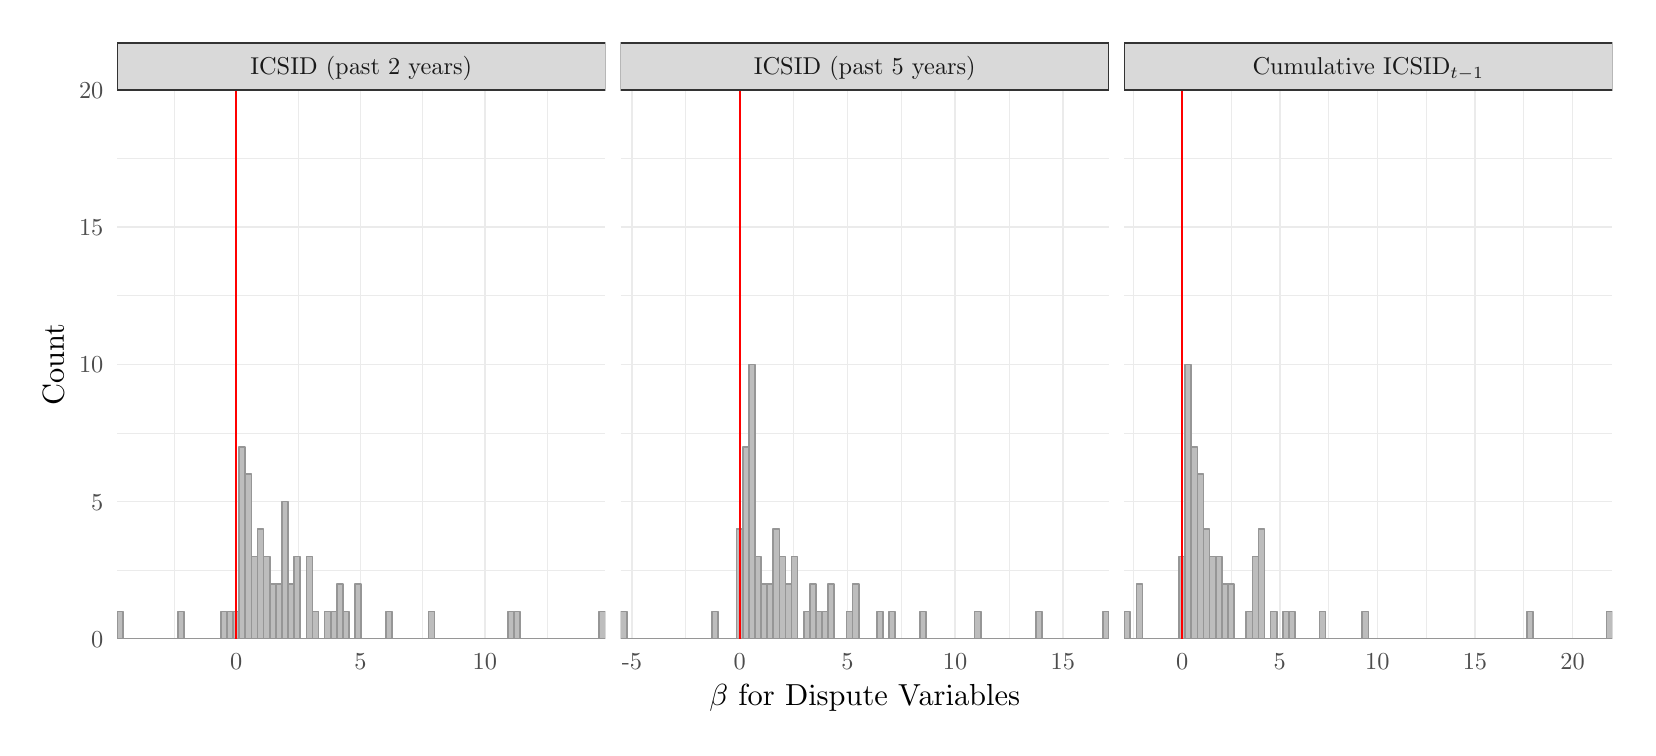
\begin{tikzpicture}[x=1pt,y=1pt]
\definecolor{fillColor}{RGB}{255,255,255}
\path[use as bounding box,fill=fillColor,fill opacity=0.00] (0,0) rectangle (578.16,252.94);
\begin{scope}
\path[clip] (  0.00,  0.00) rectangle (578.16,252.94);
\definecolor{drawColor}{RGB}{255,255,255}
\definecolor{fillColor}{RGB}{255,255,255}

\path[draw=drawColor,line width= 0.6pt,line join=round,line cap=round,fill=fillColor] (  0.00, -0.00) rectangle (578.16,252.94);
\end{scope}
\begin{scope}
\path[clip] ( 32.32, 32.09) rectangle (208.77,230.38);
\definecolor{fillColor}{RGB}{255,255,255}

\path[fill=fillColor] ( 32.32, 32.09) rectangle (208.77,230.38);
\definecolor{drawColor}{gray}{0.92}

\path[draw=drawColor,line width= 0.3pt,line join=round] ( 32.32, 56.87) --
	(208.77, 56.87);

\path[draw=drawColor,line width= 0.3pt,line join=round] ( 32.32,106.45) --
	(208.77,106.45);

\path[draw=drawColor,line width= 0.3pt,line join=round] ( 32.32,156.02) --
	(208.77,156.02);

\path[draw=drawColor,line width= 0.3pt,line join=round] ( 32.32,205.60) --
	(208.77,205.60);

\path[draw=drawColor,line width= 0.3pt,line join=round] ( 52.87, 32.09) --
	( 52.87,230.38);

\path[draw=drawColor,line width= 0.3pt,line join=round] ( 97.79, 32.09) --
	( 97.79,230.38);

\path[draw=drawColor,line width= 0.3pt,line join=round] (142.71, 32.09) --
	(142.71,230.38);

\path[draw=drawColor,line width= 0.3pt,line join=round] (187.63, 32.09) --
	(187.63,230.38);

\path[draw=drawColor,line width= 0.6pt,line join=round] ( 32.32, 32.09) --
	(208.77, 32.09);

\path[draw=drawColor,line width= 0.6pt,line join=round] ( 32.32, 81.66) --
	(208.77, 81.66);

\path[draw=drawColor,line width= 0.6pt,line join=round] ( 32.32,131.24) --
	(208.77,131.24);

\path[draw=drawColor,line width= 0.6pt,line join=round] ( 32.32,180.81) --
	(208.77,180.81);

\path[draw=drawColor,line width= 0.6pt,line join=round] ( 32.32,230.38) --
	(208.77,230.38);

\path[draw=drawColor,line width= 0.6pt,line join=round] ( 75.33, 32.09) --
	( 75.33,230.38);

\path[draw=drawColor,line width= 0.6pt,line join=round] (120.25, 32.09) --
	(120.25,230.38);

\path[draw=drawColor,line width= 0.6pt,line join=round] (165.17, 32.09) --
	(165.17,230.38);
\definecolor{drawColor}{gray}{0.59}
\definecolor{fillColor}{gray}{0.74}

\path[draw=drawColor,line width= 0.6pt,line join=round,fill=fillColor] ( 32.32, 32.09) rectangle ( 34.53, 42.00);

\path[draw=drawColor,line width= 0.6pt,line join=round,fill=fillColor] ( 34.53, 32.09) rectangle ( 36.73, 32.09);

\path[draw=drawColor,line width= 0.6pt,line join=round,fill=fillColor] ( 36.73, 32.09) rectangle ( 38.94, 32.09);

\path[draw=drawColor,line width= 0.6pt,line join=round,fill=fillColor] ( 38.94, 32.09) rectangle ( 41.15, 32.09);

\path[draw=drawColor,line width= 0.6pt,line join=round,fill=fillColor] ( 41.15, 32.09) rectangle ( 43.35, 32.09);

\path[draw=drawColor,line width= 0.6pt,line join=round,fill=fillColor] ( 43.35, 32.09) rectangle ( 45.56, 32.09);

\path[draw=drawColor,line width= 0.6pt,line join=round,fill=fillColor] ( 45.56, 32.09) rectangle ( 47.76, 32.09);

\path[draw=drawColor,line width= 0.6pt,line join=round,fill=fillColor] ( 47.76, 32.09) rectangle ( 49.97, 32.09);

\path[draw=drawColor,line width= 0.6pt,line join=round,fill=fillColor] ( 49.97, 32.09) rectangle ( 52.17, 32.09);

\path[draw=drawColor,line width= 0.6pt,line join=round,fill=fillColor] ( 52.17, 32.09) rectangle ( 54.38, 32.09);

\path[draw=drawColor,line width= 0.6pt,line join=round,fill=fillColor] ( 54.38, 32.09) rectangle ( 56.59, 42.00);

\path[draw=drawColor,line width= 0.6pt,line join=round,fill=fillColor] ( 56.59, 32.09) rectangle ( 58.79, 32.09);

\path[draw=drawColor,line width= 0.6pt,line join=round,fill=fillColor] ( 58.79, 32.09) rectangle ( 61.00, 32.09);

\path[draw=drawColor,line width= 0.6pt,line join=round,fill=fillColor] ( 61.00, 32.09) rectangle ( 63.20, 32.09);

\path[draw=drawColor,line width= 0.6pt,line join=round,fill=fillColor] ( 63.20, 32.09) rectangle ( 65.41, 32.09);

\path[draw=drawColor,line width= 0.6pt,line join=round,fill=fillColor] ( 65.41, 32.09) rectangle ( 67.61, 32.09);

\path[draw=drawColor,line width= 0.6pt,line join=round,fill=fillColor] ( 67.61, 32.09) rectangle ( 69.82, 32.09);

\path[draw=drawColor,line width= 0.6pt,line join=round,fill=fillColor] ( 69.82, 32.09) rectangle ( 72.02, 42.00);

\path[draw=drawColor,line width= 0.6pt,line join=round,fill=fillColor] ( 72.02, 32.09) rectangle ( 74.23, 42.00);

\path[draw=drawColor,line width= 0.6pt,line join=round,fill=fillColor] ( 74.23, 32.09) rectangle ( 76.44, 42.00);

\path[draw=drawColor,line width= 0.6pt,line join=round,fill=fillColor] ( 76.44, 32.09) rectangle ( 78.64,101.49);

\path[draw=drawColor,line width= 0.6pt,line join=round,fill=fillColor] ( 78.64, 32.09) rectangle ( 80.85, 91.58);

\path[draw=drawColor,line width= 0.6pt,line join=round,fill=fillColor] ( 80.85, 32.09) rectangle ( 83.05, 61.83);

\path[draw=drawColor,line width= 0.6pt,line join=round,fill=fillColor] ( 83.05, 32.09) rectangle ( 85.26, 71.75);

\path[draw=drawColor,line width= 0.6pt,line join=round,fill=fillColor] ( 85.26, 32.09) rectangle ( 87.46, 61.83);

\path[draw=drawColor,line width= 0.6pt,line join=round,fill=fillColor] ( 87.46, 32.09) rectangle ( 89.67, 51.92);

\path[draw=drawColor,line width= 0.6pt,line join=round,fill=fillColor] ( 89.67, 32.09) rectangle ( 91.87, 51.92);

\path[draw=drawColor,line width= 0.6pt,line join=round,fill=fillColor] ( 91.87, 32.09) rectangle ( 94.08, 81.66);

\path[draw=drawColor,line width= 0.6pt,line join=round,fill=fillColor] ( 94.08, 32.09) rectangle ( 96.29, 51.92);

\path[draw=drawColor,line width= 0.6pt,line join=round,fill=fillColor] ( 96.29, 32.09) rectangle ( 98.49, 61.83);

\path[draw=drawColor,line width= 0.6pt,line join=round,fill=fillColor] ( 98.49, 32.09) rectangle (100.70, 32.09);

\path[draw=drawColor,line width= 0.6pt,line join=round,fill=fillColor] (100.70, 32.09) rectangle (102.90, 61.83);

\path[draw=drawColor,line width= 0.6pt,line join=round,fill=fillColor] (102.90, 32.09) rectangle (105.11, 42.00);

\path[draw=drawColor,line width= 0.6pt,line join=round,fill=fillColor] (105.11, 32.09) rectangle (107.31, 32.09);

\path[draw=drawColor,line width= 0.6pt,line join=round,fill=fillColor] (107.31, 32.09) rectangle (109.52, 42.00);

\path[draw=drawColor,line width= 0.6pt,line join=round,fill=fillColor] (109.52, 32.09) rectangle (111.72, 42.00);

\path[draw=drawColor,line width= 0.6pt,line join=round,fill=fillColor] (111.72, 32.09) rectangle (113.93, 51.92);

\path[draw=drawColor,line width= 0.6pt,line join=round,fill=fillColor] (113.93, 32.09) rectangle (116.14, 42.00);

\path[draw=drawColor,line width= 0.6pt,line join=round,fill=fillColor] (116.14, 32.09) rectangle (118.34, 32.09);

\path[draw=drawColor,line width= 0.6pt,line join=round,fill=fillColor] (118.34, 32.09) rectangle (120.55, 51.92);

\path[draw=drawColor,line width= 0.6pt,line join=round,fill=fillColor] (120.55, 32.09) rectangle (122.75, 32.09);

\path[draw=drawColor,line width= 0.6pt,line join=round,fill=fillColor] (122.75, 32.09) rectangle (124.96, 32.09);

\path[draw=drawColor,line width= 0.6pt,line join=round,fill=fillColor] (124.96, 32.09) rectangle (127.16, 32.09);

\path[draw=drawColor,line width= 0.6pt,line join=round,fill=fillColor] (127.16, 32.09) rectangle (129.37, 32.09);

\path[draw=drawColor,line width= 0.6pt,line join=round,fill=fillColor] (129.37, 32.09) rectangle (131.57, 42.00);

\path[draw=drawColor,line width= 0.6pt,line join=round,fill=fillColor] (131.57, 32.09) rectangle (133.78, 32.09);

\path[draw=drawColor,line width= 0.6pt,line join=round,fill=fillColor] (133.78, 32.09) rectangle (135.99, 32.09);

\path[draw=drawColor,line width= 0.6pt,line join=round,fill=fillColor] (135.99, 32.09) rectangle (138.19, 32.09);

\path[draw=drawColor,line width= 0.6pt,line join=round,fill=fillColor] (138.19, 32.09) rectangle (140.40, 32.09);

\path[draw=drawColor,line width= 0.6pt,line join=round,fill=fillColor] (140.40, 32.09) rectangle (142.60, 32.09);

\path[draw=drawColor,line width= 0.6pt,line join=round,fill=fillColor] (142.60, 32.09) rectangle (144.81, 32.09);

\path[draw=drawColor,line width= 0.6pt,line join=round,fill=fillColor] (144.81, 32.09) rectangle (147.01, 42.00);

\path[draw=drawColor,line width= 0.6pt,line join=round,fill=fillColor] (147.01, 32.09) rectangle (149.22, 32.09);

\path[draw=drawColor,line width= 0.6pt,line join=round,fill=fillColor] (149.22, 32.09) rectangle (151.42, 32.09);

\path[draw=drawColor,line width= 0.6pt,line join=round,fill=fillColor] (151.42, 32.09) rectangle (153.63, 32.09);

\path[draw=drawColor,line width= 0.6pt,line join=round,fill=fillColor] (153.63, 32.09) rectangle (155.84, 32.09);

\path[draw=drawColor,line width= 0.6pt,line join=round,fill=fillColor] (155.84, 32.09) rectangle (158.04, 32.09);

\path[draw=drawColor,line width= 0.6pt,line join=round,fill=fillColor] (158.04, 32.09) rectangle (160.25, 32.09);

\path[draw=drawColor,line width= 0.6pt,line join=round,fill=fillColor] (160.25, 32.09) rectangle (162.45, 32.09);

\path[draw=drawColor,line width= 0.6pt,line join=round,fill=fillColor] (162.45, 32.09) rectangle (164.66, 32.09);

\path[draw=drawColor,line width= 0.6pt,line join=round,fill=fillColor] (164.66, 32.09) rectangle (166.86, 32.09);

\path[draw=drawColor,line width= 0.6pt,line join=round,fill=fillColor] (166.86, 32.09) rectangle (169.07, 32.09);

\path[draw=drawColor,line width= 0.6pt,line join=round,fill=fillColor] (169.07, 32.09) rectangle (171.27, 32.09);

\path[draw=drawColor,line width= 0.6pt,line join=round,fill=fillColor] (171.27, 32.09) rectangle (173.48, 32.09);

\path[draw=drawColor,line width= 0.6pt,line join=round,fill=fillColor] (173.48, 32.09) rectangle (175.69, 42.00);

\path[draw=drawColor,line width= 0.6pt,line join=round,fill=fillColor] (175.69, 32.09) rectangle (177.89, 42.00);

\path[draw=drawColor,line width= 0.6pt,line join=round,fill=fillColor] (177.89, 32.09) rectangle (180.10, 32.09);

\path[draw=drawColor,line width= 0.6pt,line join=round,fill=fillColor] (180.10, 32.09) rectangle (182.30, 32.09);

\path[draw=drawColor,line width= 0.6pt,line join=round,fill=fillColor] (182.30, 32.09) rectangle (184.51, 32.09);

\path[draw=drawColor,line width= 0.6pt,line join=round,fill=fillColor] (184.51, 32.09) rectangle (186.71, 32.09);

\path[draw=drawColor,line width= 0.6pt,line join=round,fill=fillColor] (186.71, 32.09) rectangle (188.92, 32.09);

\path[draw=drawColor,line width= 0.6pt,line join=round,fill=fillColor] (188.92, 32.09) rectangle (191.12, 32.09);

\path[draw=drawColor,line width= 0.6pt,line join=round,fill=fillColor] (191.12, 32.09) rectangle (193.33, 32.09);

\path[draw=drawColor,line width= 0.6pt,line join=round,fill=fillColor] (193.33, 32.09) rectangle (195.54, 32.09);

\path[draw=drawColor,line width= 0.6pt,line join=round,fill=fillColor] (195.54, 32.09) rectangle (197.74, 32.09);

\path[draw=drawColor,line width= 0.6pt,line join=round,fill=fillColor] (197.74, 32.09) rectangle (199.95, 32.09);

\path[draw=drawColor,line width= 0.6pt,line join=round,fill=fillColor] (199.95, 32.09) rectangle (202.15, 32.09);

\path[draw=drawColor,line width= 0.6pt,line join=round,fill=fillColor] (202.15, 32.09) rectangle (204.36, 32.09);

\path[draw=drawColor,line width= 0.6pt,line join=round,fill=fillColor] (204.36, 32.09) rectangle (206.56, 32.09);

\path[draw=drawColor,line width= 0.6pt,line join=round,fill=fillColor] (206.56, 32.09) rectangle (208.77, 42.00);
\definecolor{drawColor}{RGB}{255,0,0}

\path[draw=drawColor,line width= 0.6pt,line join=round] ( 75.33, 32.09) -- ( 75.33,230.38);
\end{scope}
\begin{scope}
\path[clip] (214.27, 32.09) rectangle (390.71,230.38);
\definecolor{fillColor}{RGB}{255,255,255}

\path[fill=fillColor] (214.27, 32.09) rectangle (390.71,230.38);
\definecolor{drawColor}{gray}{0.92}

\path[draw=drawColor,line width= 0.3pt,line join=round] (214.27, 56.87) --
	(390.71, 56.87);

\path[draw=drawColor,line width= 0.3pt,line join=round] (214.27,106.45) --
	(390.71,106.45);

\path[draw=drawColor,line width= 0.3pt,line join=round] (214.27,156.02) --
	(390.71,156.02);

\path[draw=drawColor,line width= 0.3pt,line join=round] (214.27,205.60) --
	(390.71,205.60);

\path[draw=drawColor,line width= 0.3pt,line join=round] (237.82, 32.09) --
	(237.82,230.38);

\path[draw=drawColor,line width= 0.3pt,line join=round] (276.74, 32.09) --
	(276.74,230.38);

\path[draw=drawColor,line width= 0.3pt,line join=round] (315.65, 32.09) --
	(315.65,230.38);

\path[draw=drawColor,line width= 0.3pt,line join=round] (354.57, 32.09) --
	(354.57,230.38);

\path[draw=drawColor,line width= 0.6pt,line join=round] (214.27, 32.09) --
	(390.71, 32.09);

\path[draw=drawColor,line width= 0.6pt,line join=round] (214.27, 81.66) --
	(390.71, 81.66);

\path[draw=drawColor,line width= 0.6pt,line join=round] (214.27,131.24) --
	(390.71,131.24);

\path[draw=drawColor,line width= 0.6pt,line join=round] (214.27,180.81) --
	(390.71,180.81);

\path[draw=drawColor,line width= 0.6pt,line join=round] (214.27,230.38) --
	(390.71,230.38);

\path[draw=drawColor,line width= 0.6pt,line join=round] (218.36, 32.09) --
	(218.36,230.38);

\path[draw=drawColor,line width= 0.6pt,line join=round] (257.28, 32.09) --
	(257.28,230.38);

\path[draw=drawColor,line width= 0.6pt,line join=round] (296.19, 32.09) --
	(296.19,230.38);

\path[draw=drawColor,line width= 0.6pt,line join=round] (335.11, 32.09) --
	(335.11,230.38);

\path[draw=drawColor,line width= 0.6pt,line join=round] (374.03, 32.09) --
	(374.03,230.38);
\definecolor{drawColor}{gray}{0.59}
\definecolor{fillColor}{gray}{0.74}

\path[draw=drawColor,line width= 0.6pt,line join=round,fill=fillColor] (214.27, 32.09) rectangle (216.47, 42.00);

\path[draw=drawColor,line width= 0.6pt,line join=round,fill=fillColor] (216.47, 32.09) rectangle (218.68, 32.09);

\path[draw=drawColor,line width= 0.6pt,line join=round,fill=fillColor] (218.68, 32.09) rectangle (220.89, 32.09);

\path[draw=drawColor,line width= 0.6pt,line join=round,fill=fillColor] (220.89, 32.09) rectangle (223.09, 32.09);

\path[draw=drawColor,line width= 0.6pt,line join=round,fill=fillColor] (223.09, 32.09) rectangle (225.30, 32.09);

\path[draw=drawColor,line width= 0.6pt,line join=round,fill=fillColor] (225.30, 32.09) rectangle (227.50, 32.09);

\path[draw=drawColor,line width= 0.6pt,line join=round,fill=fillColor] (227.50, 32.09) rectangle (229.71, 32.09);

\path[draw=drawColor,line width= 0.6pt,line join=round,fill=fillColor] (229.71, 32.09) rectangle (231.91, 32.09);

\path[draw=drawColor,line width= 0.6pt,line join=round,fill=fillColor] (231.91, 32.09) rectangle (234.12, 32.09);

\path[draw=drawColor,line width= 0.6pt,line join=round,fill=fillColor] (234.12, 32.09) rectangle (236.32, 32.09);

\path[draw=drawColor,line width= 0.6pt,line join=round,fill=fillColor] (236.32, 32.09) rectangle (238.53, 32.09);

\path[draw=drawColor,line width= 0.6pt,line join=round,fill=fillColor] (238.53, 32.09) rectangle (240.74, 32.09);

\path[draw=drawColor,line width= 0.6pt,line join=round,fill=fillColor] (240.74, 32.09) rectangle (242.94, 32.09);

\path[draw=drawColor,line width= 0.6pt,line join=round,fill=fillColor] (242.94, 32.09) rectangle (245.15, 32.09);

\path[draw=drawColor,line width= 0.6pt,line join=round,fill=fillColor] (245.15, 32.09) rectangle (247.35, 32.09);

\path[draw=drawColor,line width= 0.6pt,line join=round,fill=fillColor] (247.35, 32.09) rectangle (249.56, 42.00);

\path[draw=drawColor,line width= 0.6pt,line join=round,fill=fillColor] (249.56, 32.09) rectangle (251.76, 32.09);

\path[draw=drawColor,line width= 0.6pt,line join=round,fill=fillColor] (251.76, 32.09) rectangle (253.97, 32.09);

\path[draw=drawColor,line width= 0.6pt,line join=round,fill=fillColor] (253.97, 32.09) rectangle (256.18, 32.09);

\path[draw=drawColor,line width= 0.6pt,line join=round,fill=fillColor] (256.18, 32.09) rectangle (258.38, 71.75);

\path[draw=drawColor,line width= 0.6pt,line join=round,fill=fillColor] (258.38, 32.09) rectangle (260.59,101.49);

\path[draw=drawColor,line width= 0.6pt,line join=round,fill=fillColor] (260.59, 32.09) rectangle (262.79,131.24);

\path[draw=drawColor,line width= 0.6pt,line join=round,fill=fillColor] (262.79, 32.09) rectangle (265.00, 61.83);

\path[draw=drawColor,line width= 0.6pt,line join=round,fill=fillColor] (265.00, 32.09) rectangle (267.20, 51.92);

\path[draw=drawColor,line width= 0.6pt,line join=round,fill=fillColor] (267.20, 32.09) rectangle (269.41, 51.92);

\path[draw=drawColor,line width= 0.6pt,line join=round,fill=fillColor] (269.41, 32.09) rectangle (271.61, 71.75);

\path[draw=drawColor,line width= 0.6pt,line join=round,fill=fillColor] (271.61, 32.09) rectangle (273.82, 61.83);

\path[draw=drawColor,line width= 0.6pt,line join=round,fill=fillColor] (273.82, 32.09) rectangle (276.03, 51.92);

\path[draw=drawColor,line width= 0.6pt,line join=round,fill=fillColor] (276.03, 32.09) rectangle (278.23, 61.83);

\path[draw=drawColor,line width= 0.6pt,line join=round,fill=fillColor] (278.23, 32.09) rectangle (280.44, 32.09);

\path[draw=drawColor,line width= 0.6pt,line join=round,fill=fillColor] (280.44, 32.09) rectangle (282.64, 42.00);

\path[draw=drawColor,line width= 0.6pt,line join=round,fill=fillColor] (282.64, 32.09) rectangle (284.85, 51.92);

\path[draw=drawColor,line width= 0.6pt,line join=round,fill=fillColor] (284.85, 32.09) rectangle (287.05, 42.00);

\path[draw=drawColor,line width= 0.6pt,line join=round,fill=fillColor] (287.05, 32.09) rectangle (289.26, 42.00);

\path[draw=drawColor,line width= 0.6pt,line join=round,fill=fillColor] (289.26, 32.09) rectangle (291.46, 51.92);

\path[draw=drawColor,line width= 0.6pt,line join=round,fill=fillColor] (291.46, 32.09) rectangle (293.67, 32.09);

\path[draw=drawColor,line width= 0.6pt,line join=round,fill=fillColor] (293.67, 32.09) rectangle (295.88, 32.09);

\path[draw=drawColor,line width= 0.6pt,line join=round,fill=fillColor] (295.88, 32.09) rectangle (298.08, 42.00);

\path[draw=drawColor,line width= 0.6pt,line join=round,fill=fillColor] (298.08, 32.09) rectangle (300.29, 51.92);

\path[draw=drawColor,line width= 0.6pt,line join=round,fill=fillColor] (300.29, 32.09) rectangle (302.49, 32.09);

\path[draw=drawColor,line width= 0.6pt,line join=round,fill=fillColor] (302.49, 32.09) rectangle (304.70, 32.09);

\path[draw=drawColor,line width= 0.6pt,line join=round,fill=fillColor] (304.70, 32.09) rectangle (306.90, 32.09);

\path[draw=drawColor,line width= 0.6pt,line join=round,fill=fillColor] (306.90, 32.09) rectangle (309.11, 42.00);

\path[draw=drawColor,line width= 0.6pt,line join=round,fill=fillColor] (309.11, 32.09) rectangle (311.31, 32.09);

\path[draw=drawColor,line width= 0.6pt,line join=round,fill=fillColor] (311.31, 32.09) rectangle (313.52, 42.00);

\path[draw=drawColor,line width= 0.6pt,line join=round,fill=fillColor] (313.52, 32.09) rectangle (315.73, 32.09);

\path[draw=drawColor,line width= 0.6pt,line join=round,fill=fillColor] (315.73, 32.09) rectangle (317.93, 32.09);

\path[draw=drawColor,line width= 0.6pt,line join=round,fill=fillColor] (317.93, 32.09) rectangle (320.14, 32.09);

\path[draw=drawColor,line width= 0.6pt,line join=round,fill=fillColor] (320.14, 32.09) rectangle (322.34, 32.09);

\path[draw=drawColor,line width= 0.6pt,line join=round,fill=fillColor] (322.34, 32.09) rectangle (324.55, 42.00);

\path[draw=drawColor,line width= 0.6pt,line join=round,fill=fillColor] (324.55, 32.09) rectangle (326.75, 32.09);

\path[draw=drawColor,line width= 0.6pt,line join=round,fill=fillColor] (326.75, 32.09) rectangle (328.96, 32.09);

\path[draw=drawColor,line width= 0.6pt,line join=round,fill=fillColor] (328.96, 32.09) rectangle (331.16, 32.09);

\path[draw=drawColor,line width= 0.6pt,line join=round,fill=fillColor] (331.16, 32.09) rectangle (333.37, 32.09);

\path[draw=drawColor,line width= 0.6pt,line join=round,fill=fillColor] (333.37, 32.09) rectangle (335.58, 32.09);

\path[draw=drawColor,line width= 0.6pt,line join=round,fill=fillColor] (335.58, 32.09) rectangle (337.78, 32.09);

\path[draw=drawColor,line width= 0.6pt,line join=round,fill=fillColor] (337.78, 32.09) rectangle (339.99, 32.09);

\path[draw=drawColor,line width= 0.6pt,line join=round,fill=fillColor] (339.99, 32.09) rectangle (342.19, 32.09);

\path[draw=drawColor,line width= 0.6pt,line join=round,fill=fillColor] (342.19, 32.09) rectangle (344.40, 42.00);

\path[draw=drawColor,line width= 0.6pt,line join=round,fill=fillColor] (344.40, 32.09) rectangle (346.60, 32.09);

\path[draw=drawColor,line width= 0.6pt,line join=round,fill=fillColor] (346.60, 32.09) rectangle (348.81, 32.09);

\path[draw=drawColor,line width= 0.6pt,line join=round,fill=fillColor] (348.81, 32.09) rectangle (351.01, 32.09);

\path[draw=drawColor,line width= 0.6pt,line join=round,fill=fillColor] (351.01, 32.09) rectangle (353.22, 32.09);

\path[draw=drawColor,line width= 0.6pt,line join=round,fill=fillColor] (353.22, 32.09) rectangle (355.43, 32.09);

\path[draw=drawColor,line width= 0.6pt,line join=round,fill=fillColor] (355.43, 32.09) rectangle (357.63, 32.09);

\path[draw=drawColor,line width= 0.6pt,line join=round,fill=fillColor] (357.63, 32.09) rectangle (359.84, 32.09);

\path[draw=drawColor,line width= 0.6pt,line join=round,fill=fillColor] (359.84, 32.09) rectangle (362.04, 32.09);

\path[draw=drawColor,line width= 0.6pt,line join=round,fill=fillColor] (362.04, 32.09) rectangle (364.25, 32.09);

\path[draw=drawColor,line width= 0.6pt,line join=round,fill=fillColor] (364.25, 32.09) rectangle (366.45, 42.00);

\path[draw=drawColor,line width= 0.6pt,line join=round,fill=fillColor] (366.45, 32.09) rectangle (368.66, 32.09);

\path[draw=drawColor,line width= 0.6pt,line join=round,fill=fillColor] (368.66, 32.09) rectangle (370.86, 32.09);

\path[draw=drawColor,line width= 0.6pt,line join=round,fill=fillColor] (370.86, 32.09) rectangle (373.07, 32.09);

\path[draw=drawColor,line width= 0.6pt,line join=round,fill=fillColor] (373.07, 32.09) rectangle (375.28, 32.09);

\path[draw=drawColor,line width= 0.6pt,line join=round,fill=fillColor] (375.28, 32.09) rectangle (377.48, 32.09);

\path[draw=drawColor,line width= 0.6pt,line join=round,fill=fillColor] (377.48, 32.09) rectangle (379.69, 32.09);

\path[draw=drawColor,line width= 0.6pt,line join=round,fill=fillColor] (379.69, 32.09) rectangle (381.89, 32.09);

\path[draw=drawColor,line width= 0.6pt,line join=round,fill=fillColor] (381.89, 32.09) rectangle (384.10, 32.09);

\path[draw=drawColor,line width= 0.6pt,line join=round,fill=fillColor] (384.10, 32.09) rectangle (386.30, 32.09);

\path[draw=drawColor,line width= 0.6pt,line join=round,fill=fillColor] (386.30, 32.09) rectangle (388.51, 32.09);

\path[draw=drawColor,line width= 0.6pt,line join=round,fill=fillColor] (388.51, 32.09) rectangle (390.71, 42.00);
\definecolor{drawColor}{RGB}{255,0,0}

\path[draw=drawColor,line width= 0.6pt,line join=round] (257.28, 32.09) -- (257.28,230.38);
\end{scope}
\begin{scope}
\path[clip] (396.21, 32.09) rectangle (572.66,230.38);
\definecolor{fillColor}{RGB}{255,255,255}

\path[fill=fillColor] (396.21, 32.09) rectangle (572.66,230.38);
\definecolor{drawColor}{gray}{0.92}

\path[draw=drawColor,line width= 0.3pt,line join=round] (396.21, 56.87) --
	(572.66, 56.87);

\path[draw=drawColor,line width= 0.3pt,line join=round] (396.21,106.45) --
	(572.66,106.45);

\path[draw=drawColor,line width= 0.3pt,line join=round] (396.21,156.02) --
	(572.66,156.02);

\path[draw=drawColor,line width= 0.3pt,line join=round] (396.21,205.60) --
	(572.66,205.60);

\path[draw=drawColor,line width= 0.3pt,line join=round] (399.53, 32.09) --
	(399.53,230.38);

\path[draw=drawColor,line width= 0.3pt,line join=round] (434.80, 32.09) --
	(434.80,230.38);

\path[draw=drawColor,line width= 0.3pt,line join=round] (470.07, 32.09) --
	(470.07,230.38);

\path[draw=drawColor,line width= 0.3pt,line join=round] (505.33, 32.09) --
	(505.33,230.38);

\path[draw=drawColor,line width= 0.3pt,line join=round] (540.60, 32.09) --
	(540.60,230.38);

\path[draw=drawColor,line width= 0.6pt,line join=round] (396.21, 32.09) --
	(572.66, 32.09);

\path[draw=drawColor,line width= 0.6pt,line join=round] (396.21, 81.66) --
	(572.66, 81.66);

\path[draw=drawColor,line width= 0.6pt,line join=round] (396.21,131.24) --
	(572.66,131.24);

\path[draw=drawColor,line width= 0.6pt,line join=round] (396.21,180.81) --
	(572.66,180.81);

\path[draw=drawColor,line width= 0.6pt,line join=round] (396.21,230.38) --
	(572.66,230.38);

\path[draw=drawColor,line width= 0.6pt,line join=round] (417.17, 32.09) --
	(417.17,230.38);

\path[draw=drawColor,line width= 0.6pt,line join=round] (452.43, 32.09) --
	(452.43,230.38);

\path[draw=drawColor,line width= 0.6pt,line join=round] (487.70, 32.09) --
	(487.70,230.38);

\path[draw=drawColor,line width= 0.6pt,line join=round] (522.97, 32.09) --
	(522.97,230.38);

\path[draw=drawColor,line width= 0.6pt,line join=round] (558.23, 32.09) --
	(558.23,230.38);
\definecolor{drawColor}{gray}{0.59}
\definecolor{fillColor}{gray}{0.74}

\path[draw=drawColor,line width= 0.6pt,line join=round,fill=fillColor] (396.21, 32.09) rectangle (398.42, 42.00);

\path[draw=drawColor,line width= 0.6pt,line join=round,fill=fillColor] (398.42, 32.09) rectangle (400.63, 32.09);

\path[draw=drawColor,line width= 0.6pt,line join=round,fill=fillColor] (400.63, 32.09) rectangle (402.83, 51.92);

\path[draw=drawColor,line width= 0.6pt,line join=round,fill=fillColor] (402.83, 32.09) rectangle (405.04, 32.09);

\path[draw=drawColor,line width= 0.6pt,line join=round,fill=fillColor] (405.04, 32.09) rectangle (407.24, 32.09);

\path[draw=drawColor,line width= 0.6pt,line join=round,fill=fillColor] (407.24, 32.09) rectangle (409.45, 32.09);

\path[draw=drawColor,line width= 0.6pt,line join=round,fill=fillColor] (409.45, 32.09) rectangle (411.65, 32.09);

\path[draw=drawColor,line width= 0.6pt,line join=round,fill=fillColor] (411.65, 32.09) rectangle (413.86, 32.09);

\path[draw=drawColor,line width= 0.6pt,line join=round,fill=fillColor] (413.86, 32.09) rectangle (416.06, 32.09);

\path[draw=drawColor,line width= 0.6pt,line join=round,fill=fillColor] (416.06, 32.09) rectangle (418.27, 61.83);

\path[draw=drawColor,line width= 0.6pt,line join=round,fill=fillColor] (418.27, 32.09) rectangle (420.48,131.24);

\path[draw=drawColor,line width= 0.6pt,line join=round,fill=fillColor] (420.48, 32.09) rectangle (422.68,101.49);

\path[draw=drawColor,line width= 0.6pt,line join=round,fill=fillColor] (422.68, 32.09) rectangle (424.89, 91.58);

\path[draw=drawColor,line width= 0.6pt,line join=round,fill=fillColor] (424.89, 32.09) rectangle (427.09, 71.75);

\path[draw=drawColor,line width= 0.6pt,line join=round,fill=fillColor] (427.09, 32.09) rectangle (429.30, 61.83);

\path[draw=drawColor,line width= 0.6pt,line join=round,fill=fillColor] (429.30, 32.09) rectangle (431.50, 61.83);

\path[draw=drawColor,line width= 0.6pt,line join=round,fill=fillColor] (431.50, 32.09) rectangle (433.71, 51.92);

\path[draw=drawColor,line width= 0.6pt,line join=round,fill=fillColor] (433.71, 32.09) rectangle (435.91, 51.92);

\path[draw=drawColor,line width= 0.6pt,line join=round,fill=fillColor] (435.91, 32.09) rectangle (438.12, 32.09);

\path[draw=drawColor,line width= 0.6pt,line join=round,fill=fillColor] (438.12, 32.09) rectangle (440.33, 32.09);

\path[draw=drawColor,line width= 0.6pt,line join=round,fill=fillColor] (440.33, 32.09) rectangle (442.53, 42.00);

\path[draw=drawColor,line width= 0.6pt,line join=round,fill=fillColor] (442.53, 32.09) rectangle (444.74, 61.83);

\path[draw=drawColor,line width= 0.6pt,line join=round,fill=fillColor] (444.74, 32.09) rectangle (446.94, 71.75);

\path[draw=drawColor,line width= 0.6pt,line join=round,fill=fillColor] (446.94, 32.09) rectangle (449.15, 32.09);

\path[draw=drawColor,line width= 0.6pt,line join=round,fill=fillColor] (449.15, 32.09) rectangle (451.35, 42.00);

\path[draw=drawColor,line width= 0.6pt,line join=round,fill=fillColor] (451.35, 32.09) rectangle (453.56, 32.09);

\path[draw=drawColor,line width= 0.6pt,line join=round,fill=fillColor] (453.56, 32.09) rectangle (455.76, 42.00);

\path[draw=drawColor,line width= 0.6pt,line join=round,fill=fillColor] (455.76, 32.09) rectangle (457.97, 42.00);

\path[draw=drawColor,line width= 0.6pt,line join=round,fill=fillColor] (457.97, 32.09) rectangle (460.18, 32.09);

\path[draw=drawColor,line width= 0.6pt,line join=round,fill=fillColor] (460.18, 32.09) rectangle (462.38, 32.09);

\path[draw=drawColor,line width= 0.6pt,line join=round,fill=fillColor] (462.38, 32.09) rectangle (464.59, 32.09);

\path[draw=drawColor,line width= 0.6pt,line join=round,fill=fillColor] (464.59, 32.09) rectangle (466.79, 32.09);

\path[draw=drawColor,line width= 0.6pt,line join=round,fill=fillColor] (466.79, 32.09) rectangle (469.00, 42.00);

\path[draw=drawColor,line width= 0.6pt,line join=round,fill=fillColor] (469.00, 32.09) rectangle (471.20, 32.09);

\path[draw=drawColor,line width= 0.6pt,line join=round,fill=fillColor] (471.20, 32.09) rectangle (473.41, 32.09);

\path[draw=drawColor,line width= 0.6pt,line join=round,fill=fillColor] (473.41, 32.09) rectangle (475.62, 32.09);

\path[draw=drawColor,line width= 0.6pt,line join=round,fill=fillColor] (475.62, 32.09) rectangle (477.82, 32.09);

\path[draw=drawColor,line width= 0.6pt,line join=round,fill=fillColor] (477.82, 32.09) rectangle (480.03, 32.09);

\path[draw=drawColor,line width= 0.6pt,line join=round,fill=fillColor] (480.03, 32.09) rectangle (482.23, 32.09);

\path[draw=drawColor,line width= 0.6pt,line join=round,fill=fillColor] (482.23, 32.09) rectangle (484.44, 42.00);

\path[draw=drawColor,line width= 0.6pt,line join=round,fill=fillColor] (484.44, 32.09) rectangle (486.64, 32.09);

\path[draw=drawColor,line width= 0.6pt,line join=round,fill=fillColor] (486.64, 32.09) rectangle (488.85, 32.09);

\path[draw=drawColor,line width= 0.6pt,line join=round,fill=fillColor] (488.85, 32.09) rectangle (491.05, 32.09);

\path[draw=drawColor,line width= 0.6pt,line join=round,fill=fillColor] (491.05, 32.09) rectangle (493.26, 32.09);

\path[draw=drawColor,line width= 0.6pt,line join=round,fill=fillColor] (493.26, 32.09) rectangle (495.47, 32.09);

\path[draw=drawColor,line width= 0.6pt,line join=round,fill=fillColor] (495.47, 32.09) rectangle (497.67, 32.09);

\path[draw=drawColor,line width= 0.6pt,line join=round,fill=fillColor] (497.67, 32.09) rectangle (499.88, 32.09);

\path[draw=drawColor,line width= 0.6pt,line join=round,fill=fillColor] (499.88, 32.09) rectangle (502.08, 32.09);

\path[draw=drawColor,line width= 0.6pt,line join=round,fill=fillColor] (502.08, 32.09) rectangle (504.29, 32.09);

\path[draw=drawColor,line width= 0.6pt,line join=round,fill=fillColor] (504.29, 32.09) rectangle (506.49, 32.09);

\path[draw=drawColor,line width= 0.6pt,line join=round,fill=fillColor] (506.49, 32.09) rectangle (508.70, 32.09);

\path[draw=drawColor,line width= 0.6pt,line join=round,fill=fillColor] (508.70, 32.09) rectangle (510.90, 32.09);

\path[draw=drawColor,line width= 0.6pt,line join=round,fill=fillColor] (510.90, 32.09) rectangle (513.11, 32.09);

\path[draw=drawColor,line width= 0.6pt,line join=round,fill=fillColor] (513.11, 32.09) rectangle (515.32, 32.09);

\path[draw=drawColor,line width= 0.6pt,line join=round,fill=fillColor] (515.32, 32.09) rectangle (517.52, 32.09);

\path[draw=drawColor,line width= 0.6pt,line join=round,fill=fillColor] (517.52, 32.09) rectangle (519.73, 32.09);

\path[draw=drawColor,line width= 0.6pt,line join=round,fill=fillColor] (519.73, 32.09) rectangle (521.93, 32.09);

\path[draw=drawColor,line width= 0.6pt,line join=round,fill=fillColor] (521.93, 32.09) rectangle (524.14, 32.09);

\path[draw=drawColor,line width= 0.6pt,line join=round,fill=fillColor] (524.14, 32.09) rectangle (526.34, 32.09);

\path[draw=drawColor,line width= 0.6pt,line join=round,fill=fillColor] (526.34, 32.09) rectangle (528.55, 32.09);

\path[draw=drawColor,line width= 0.6pt,line join=round,fill=fillColor] (528.55, 32.09) rectangle (530.75, 32.09);

\path[draw=drawColor,line width= 0.6pt,line join=round,fill=fillColor] (530.75, 32.09) rectangle (532.96, 32.09);

\path[draw=drawColor,line width= 0.6pt,line join=round,fill=fillColor] (532.96, 32.09) rectangle (535.17, 32.09);

\path[draw=drawColor,line width= 0.6pt,line join=round,fill=fillColor] (535.17, 32.09) rectangle (537.37, 32.09);

\path[draw=drawColor,line width= 0.6pt,line join=round,fill=fillColor] (537.37, 32.09) rectangle (539.58, 32.09);

\path[draw=drawColor,line width= 0.6pt,line join=round,fill=fillColor] (539.58, 32.09) rectangle (541.78, 32.09);

\path[draw=drawColor,line width= 0.6pt,line join=round,fill=fillColor] (541.78, 32.09) rectangle (543.99, 42.00);

\path[draw=drawColor,line width= 0.6pt,line join=round,fill=fillColor] (543.99, 32.09) rectangle (546.19, 32.09);

\path[draw=drawColor,line width= 0.6pt,line join=round,fill=fillColor] (546.19, 32.09) rectangle (548.40, 32.09);

\path[draw=drawColor,line width= 0.6pt,line join=round,fill=fillColor] (548.40, 32.09) rectangle (550.60, 32.09);

\path[draw=drawColor,line width= 0.6pt,line join=round,fill=fillColor] (550.60, 32.09) rectangle (552.81, 32.09);

\path[draw=drawColor,line width= 0.6pt,line join=round,fill=fillColor] (552.81, 32.09) rectangle (555.02, 32.09);

\path[draw=drawColor,line width= 0.6pt,line join=round,fill=fillColor] (555.02, 32.09) rectangle (557.22, 32.09);

\path[draw=drawColor,line width= 0.6pt,line join=round,fill=fillColor] (557.22, 32.09) rectangle (559.43, 32.09);

\path[draw=drawColor,line width= 0.6pt,line join=round,fill=fillColor] (559.43, 32.09) rectangle (561.63, 32.09);

\path[draw=drawColor,line width= 0.6pt,line join=round,fill=fillColor] (561.63, 32.09) rectangle (563.84, 32.09);

\path[draw=drawColor,line width= 0.6pt,line join=round,fill=fillColor] (563.84, 32.09) rectangle (566.04, 32.09);

\path[draw=drawColor,line width= 0.6pt,line join=round,fill=fillColor] (566.04, 32.09) rectangle (568.25, 32.09);

\path[draw=drawColor,line width= 0.6pt,line join=round,fill=fillColor] (568.25, 32.09) rectangle (570.45, 32.09);

\path[draw=drawColor,line width= 0.6pt,line join=round,fill=fillColor] (570.45, 32.09) rectangle (572.66, 42.00);
\definecolor{drawColor}{RGB}{255,0,0}

\path[draw=drawColor,line width= 0.6pt,line join=round] (417.17, 32.09) -- (417.17,230.38);
\end{scope}
\begin{scope}
\path[clip] ( 32.32,230.38) rectangle (208.77,247.44);
\definecolor{drawColor}{gray}{0.20}
\definecolor{fillColor}{gray}{0.85}

\path[draw=drawColor,line width= 0.6pt,line join=round,line cap=round,fill=fillColor] ( 32.32,230.38) rectangle (208.77,247.44);
\definecolor{drawColor}{gray}{0.10}

\node[text=drawColor,anchor=base,inner sep=0pt, outer sep=0pt, scale=  0.88] at (120.55,235.88) {ICSID  (past 2 years)};
\end{scope}
\begin{scope}
\path[clip] (214.27,230.38) rectangle (390.71,247.44);
\definecolor{drawColor}{gray}{0.20}
\definecolor{fillColor}{gray}{0.85}

\path[draw=drawColor,line width= 0.6pt,line join=round,line cap=round,fill=fillColor] (214.27,230.38) rectangle (390.71,247.44);
\definecolor{drawColor}{gray}{0.10}

\node[text=drawColor,anchor=base,inner sep=0pt, outer sep=0pt, scale=  0.88] at (302.49,235.88) {ICSID  (past 5 years)};
\end{scope}
\begin{scope}
\path[clip] (396.21,230.38) rectangle (572.66,247.44);
\definecolor{drawColor}{gray}{0.20}
\definecolor{fillColor}{gray}{0.85}

\path[draw=drawColor,line width= 0.6pt,line join=round,line cap=round,fill=fillColor] (396.21,230.38) rectangle (572.66,247.44);
\definecolor{drawColor}{gray}{0.10}

\node[text=drawColor,anchor=base,inner sep=0pt, outer sep=0pt, scale=  0.88] at (484.44,235.88) {Cumulative ICSID$_{t-1}$};
\end{scope}
\begin{scope}
\path[clip] (  0.00,  0.00) rectangle (578.16,252.94);
\definecolor{drawColor}{gray}{0.30}

\node[text=drawColor,anchor=base,inner sep=0pt, outer sep=0pt, scale=  0.88] at ( 75.33, 21.08) {0};

\node[text=drawColor,anchor=base,inner sep=0pt, outer sep=0pt, scale=  0.88] at (120.25, 21.08) {5};

\node[text=drawColor,anchor=base,inner sep=0pt, outer sep=0pt, scale=  0.88] at (165.17, 21.08) {10};
\end{scope}
\begin{scope}
\path[clip] (  0.00,  0.00) rectangle (578.16,252.94);
\definecolor{drawColor}{gray}{0.30}

\node[text=drawColor,anchor=base,inner sep=0pt, outer sep=0pt, scale=  0.88] at (218.36, 21.08) {-5};

\node[text=drawColor,anchor=base,inner sep=0pt, outer sep=0pt, scale=  0.88] at (257.28, 21.08) {0};

\node[text=drawColor,anchor=base,inner sep=0pt, outer sep=0pt, scale=  0.88] at (296.19, 21.08) {5};

\node[text=drawColor,anchor=base,inner sep=0pt, outer sep=0pt, scale=  0.88] at (335.11, 21.08) {10};

\node[text=drawColor,anchor=base,inner sep=0pt, outer sep=0pt, scale=  0.88] at (374.03, 21.08) {15};
\end{scope}
\begin{scope}
\path[clip] (  0.00,  0.00) rectangle (578.16,252.94);
\definecolor{drawColor}{gray}{0.30}

\node[text=drawColor,anchor=base,inner sep=0pt, outer sep=0pt, scale=  0.88] at (417.17, 21.08) {0};

\node[text=drawColor,anchor=base,inner sep=0pt, outer sep=0pt, scale=  0.88] at (452.43, 21.08) {5};

\node[text=drawColor,anchor=base,inner sep=0pt, outer sep=0pt, scale=  0.88] at (487.70, 21.08) {10};

\node[text=drawColor,anchor=base,inner sep=0pt, outer sep=0pt, scale=  0.88] at (522.97, 21.08) {15};

\node[text=drawColor,anchor=base,inner sep=0pt, outer sep=0pt, scale=  0.88] at (558.23, 21.08) {20};
\end{scope}
\begin{scope}
\path[clip] (  0.00,  0.00) rectangle (578.16,252.94);
\definecolor{drawColor}{gray}{0.30}

\node[text=drawColor,anchor=base east,inner sep=0pt, outer sep=0pt, scale=  0.88] at ( 27.37, 29.06) {0};

\node[text=drawColor,anchor=base east,inner sep=0pt, outer sep=0pt, scale=  0.88] at ( 27.37, 78.63) {5};

\node[text=drawColor,anchor=base east,inner sep=0pt, outer sep=0pt, scale=  0.88] at ( 27.37,128.20) {10};

\node[text=drawColor,anchor=base east,inner sep=0pt, outer sep=0pt, scale=  0.88] at ( 27.37,177.78) {15};

\node[text=drawColor,anchor=base east,inner sep=0pt, outer sep=0pt, scale=  0.88] at ( 27.37,227.35) {20};
\end{scope}
\begin{scope}
\path[clip] (  0.00,  0.00) rectangle (578.16,252.94);
\definecolor{drawColor}{RGB}{0,0,0}

\node[text=drawColor,anchor=base,inner sep=0pt, outer sep=0pt, scale=  1.10] at (302.49,  8.00) {$\beta$ for Dispute Variables};
\end{scope}
\begin{scope}
\path[clip] (  0.00,  0.00) rectangle (578.16,252.94);
\definecolor{drawColor}{RGB}{0,0,0}

\node[text=drawColor,rotate= 90.00,anchor=base,inner sep=0pt, outer sep=0pt, scale=  1.10] at ( 13.08,131.24) {Count};
\end{scope}
\end{tikzpicture}
}	
\end{figure}

\end{frame}
%%%%%%%%%%%%%%%%%%%%%%%%%%%%%%%%%%%%%%%%%

%%%%%%%%%%%%%%%%%%%%%%%%%%%%%%%%%%%%%%%%%
\begin{frame}
\frametitle{Adding in some controls...}

% \pause
\begin{figure}[ht]
	\centering
	\vspace{-5mm}
	\resizebox{1\textwidth}{!}{% Created by tikzDevice version 0.6.1 on 2016-03-17 13:37:26
% !TEX encoding = UTF-8 Unicode
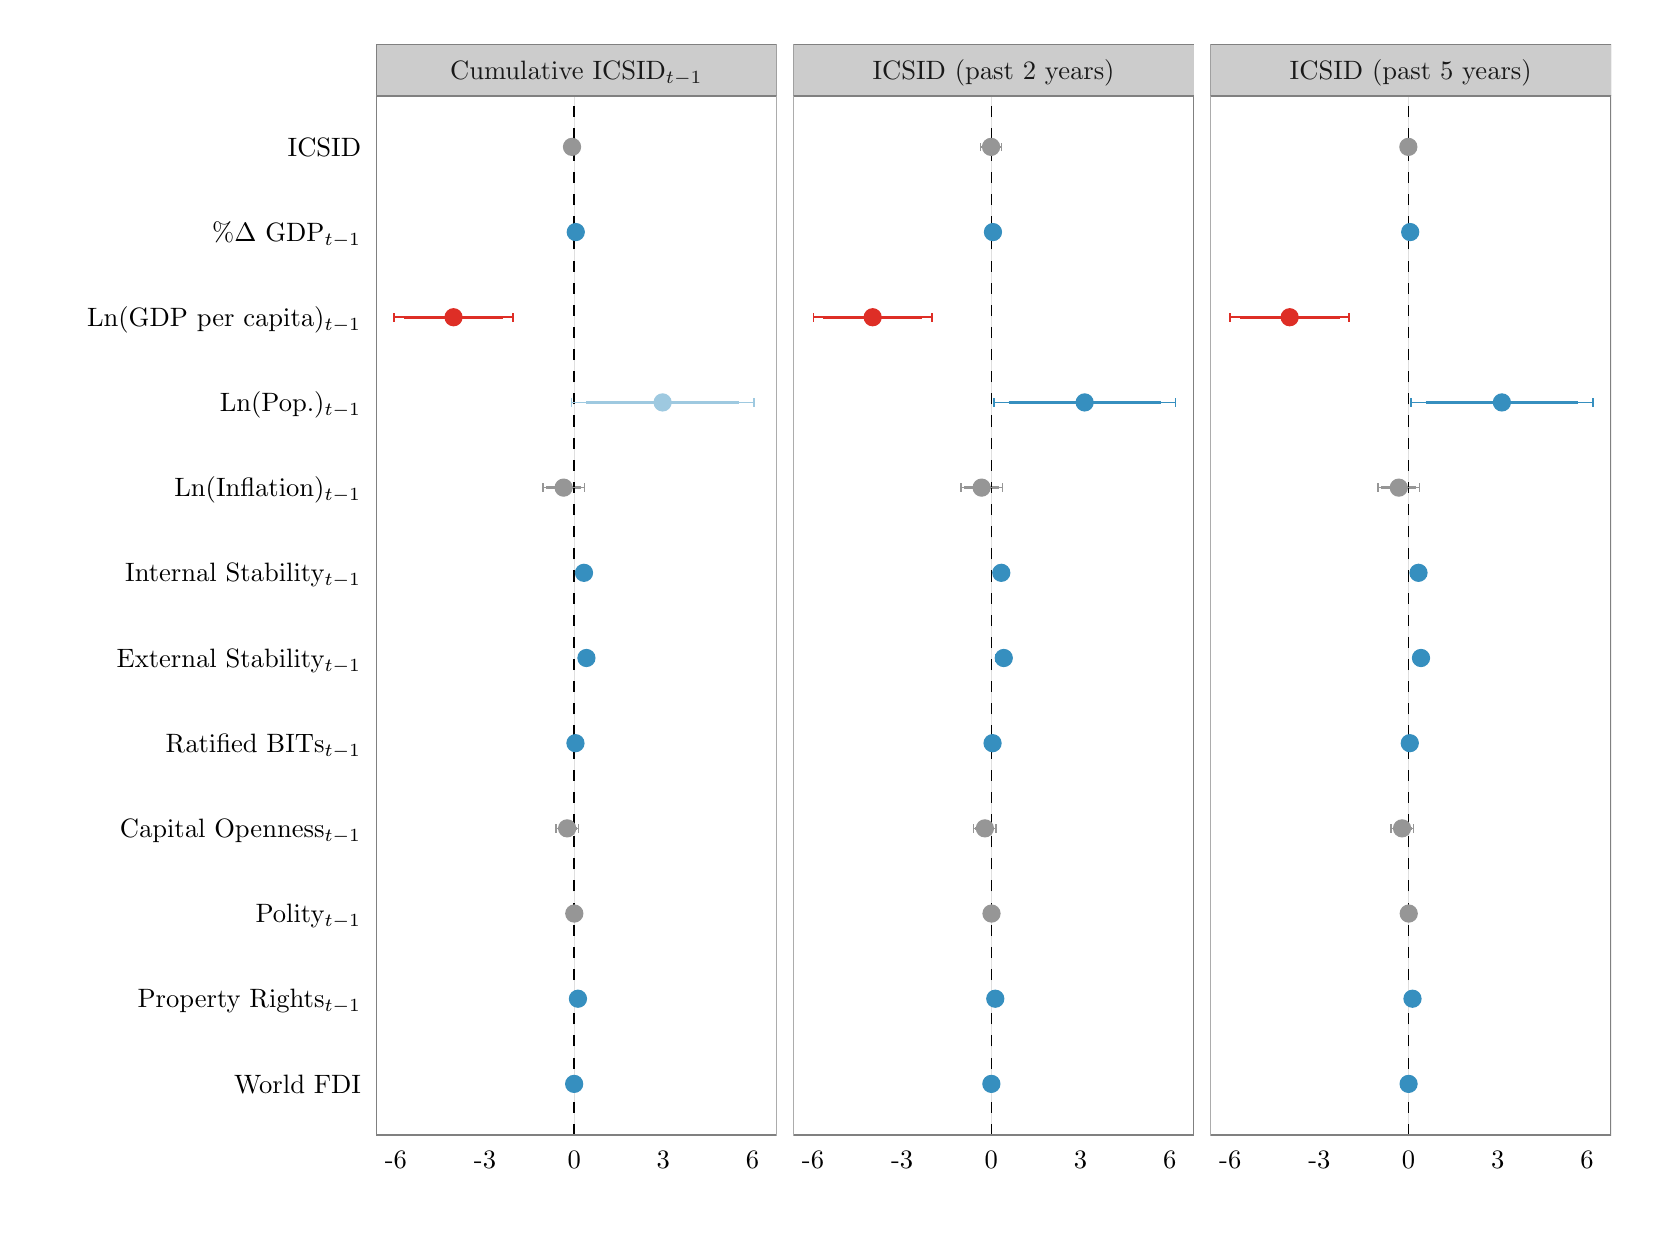
\begin{tikzpicture}[x=1pt,y=1pt]
\definecolor[named]{drawColor}{rgb}{0.00,0.00,0.00}
\definecolor[named]{fillColor}{rgb}{1.00,1.00,1.00}
\fill[color=fillColor,] (0,0) rectangle (578.16,433.62);
\begin{scope}
\path[clip] (  0.00,  0.00) rectangle (578.16,433.62);
\end{scope}
\begin{scope}
\path[clip] (  0.00,  0.00) rectangle (578.16,433.62);
\end{scope}
\begin{scope}
\path[clip] (  0.00,  0.00) rectangle (578.16,433.62);
\end{scope}
\begin{scope}
\path[clip] (  0.00,  0.00) rectangle (578.16,433.62);
\end{scope}
\begin{scope}
\path[clip] (  0.00,  0.00) rectangle (578.16,433.62);
\end{scope}
\begin{scope}
\path[clip] (  0.00,  0.00) rectangle (578.16,433.62);
\end{scope}
\begin{scope}
\path[clip] (  0.00,  0.00) rectangle (578.16,433.62);
\end{scope}
\begin{scope}
\path[clip] (  0.00,  0.00) rectangle (578.16,433.62);
\end{scope}
\begin{scope}
\path[clip] (  0.00,  0.00) rectangle (578.16,433.62);
\end{scope}
\begin{scope}
\path[clip] (  0.00,  0.00) rectangle (578.16,433.62);
\end{scope}
\begin{scope}
\path[clip] (  0.00,  0.00) rectangle (578.16,433.62);
\end{scope}
\begin{scope}
\path[clip] (  0.00,  0.00) rectangle (578.16,433.62);
\end{scope}
\begin{scope}
\path[clip] (  0.00,  0.00) rectangle (578.16,433.62);
\end{scope}
\begin{scope}
\path[clip] (  0.00,  0.00) rectangle (578.16,433.62);
\definecolor[named]{drawColor}{rgb}{1.00,1.00,1.00}
\definecolor[named]{fillColor}{rgb}{1.00,1.00,1.00}

\draw[color=drawColor,line width= 0.6pt,line cap=round,line join=round,fill=fillColor,] (  0.00,  0.00) rectangle (578.16,433.62);
\end{scope}
\begin{scope}
\path[clip] (  0.00,  0.00) rectangle (578.16,433.62);
\end{scope}
\begin{scope}
\path[clip] (125.88, 33.48) rectangle (270.64,409.01);
\definecolor[named]{fillColor}{rgb}{1.00,1.00,1.00}

\draw[fill=fillColor,draw opacity=0.00,] (125.88, 33.48) rectangle (270.64,409.01);
\definecolor[named]{drawColor}{rgb}{0.59,0.59,0.59}
\definecolor[named]{fillColor}{rgb}{0.59,0.59,0.59}

\draw[color=drawColor,line width= 0.3pt,line join=round,fill=fillColor,fill opacity=0.30,draw opacity=0.30,] (195.31,390.54) -- (198.08,390.54);
\definecolor[named]{drawColor}{rgb}{0.21,0.56,0.75}
\definecolor[named]{fillColor}{rgb}{0.21,0.56,0.75}

\draw[color=drawColor,line width= 0.3pt,line join=round,fill=fillColor,fill opacity=0.30,draw opacity=0.30,] (197.48,359.76) -- (198.63,359.76);
\definecolor[named]{drawColor}{rgb}{0.87,0.18,0.15}
\definecolor[named]{fillColor}{rgb}{0.87,0.18,0.15}

\draw[color=drawColor,line width= 0.3pt,line join=round,fill=fillColor,fill opacity=0.30,draw opacity=0.30,] (132.46,328.98) -- (175.30,328.98);
\definecolor[named]{drawColor}{rgb}{0.62,0.79,0.88}
\definecolor[named]{fillColor}{rgb}{0.62,0.79,0.88}

\draw[color=drawColor,line width= 0.3pt,line join=round,fill=fillColor,fill opacity=0.30,draw opacity=0.30,] (196.52,298.20) -- (262.34,298.20);
\definecolor[named]{drawColor}{rgb}{0.59,0.59,0.59}
\definecolor[named]{fillColor}{rgb}{0.59,0.59,0.59}

\draw[color=drawColor,line width= 0.3pt,line join=round,fill=fillColor,fill opacity=0.30,draw opacity=0.30,] (186.15,267.41) -- (201.19,267.41);
\definecolor[named]{drawColor}{rgb}{0.21,0.56,0.75}
\definecolor[named]{fillColor}{rgb}{0.21,0.56,0.75}

\draw[color=drawColor,line width= 0.3pt,line join=round,fill=fillColor,fill opacity=0.30,draw opacity=0.30,] (198.40,236.63) -- (203.63,236.63);

\draw[color=drawColor,line width= 0.3pt,line join=round,fill=fillColor,fill opacity=0.30,draw opacity=0.30,] (199.15,205.85) -- (204.66,205.85);

\draw[color=drawColor,line width= 0.3pt,line join=round,fill=fillColor,fill opacity=0.30,draw opacity=0.30,] (197.51,175.07) -- (198.37,175.07);
\definecolor[named]{drawColor}{rgb}{0.59,0.59,0.59}
\definecolor[named]{fillColor}{rgb}{0.59,0.59,0.59}

\draw[color=drawColor,line width= 0.3pt,line join=round,fill=fillColor,fill opacity=0.30,draw opacity=0.30,] (190.83,144.29) -- (199.05,144.29);

\draw[color=drawColor,line width= 0.3pt,line join=round,fill=fillColor,fill opacity=0.30,draw opacity=0.30,] (197.25,113.51) -- (197.79,113.51);
\definecolor[named]{drawColor}{rgb}{0.21,0.56,0.75}
\definecolor[named]{fillColor}{rgb}{0.21,0.56,0.75}

\draw[color=drawColor,line width= 0.3pt,line join=round,fill=fillColor,fill opacity=0.30,draw opacity=0.30,] (197.58, 82.73) -- (200.10, 82.73);

\draw[color=drawColor,line width= 0.3pt,line join=round,fill=fillColor,fill opacity=0.30,draw opacity=0.30,] (197.47, 51.95) -- (197.47, 51.95);
\definecolor[named]{drawColor}{rgb}{0.59,0.59,0.59}
\definecolor[named]{fillColor}{rgb}{0.59,0.59,0.59}

\draw[color=drawColor,line width= 1.1pt,line join=round,fill=fillColor,] (195.54,390.54) -- (197.86,390.54);
\definecolor[named]{drawColor}{rgb}{0.21,0.56,0.75}
\definecolor[named]{fillColor}{rgb}{0.21,0.56,0.75}

\draw[color=drawColor,line width= 1.1pt,line join=round,fill=fillColor,] (197.57,359.76) -- (198.53,359.76);
\definecolor[named]{drawColor}{rgb}{0.87,0.18,0.15}
\definecolor[named]{fillColor}{rgb}{0.87,0.18,0.15}

\draw[color=drawColor,line width= 1.1pt,line join=round,fill=fillColor,] (135.90,328.98) -- (171.86,328.98);
\definecolor[named]{drawColor}{rgb}{0.62,0.79,0.88}
\definecolor[named]{fillColor}{rgb}{0.62,0.79,0.88}

\draw[color=drawColor,line width= 1.1pt,line join=round,fill=fillColor,] (201.81,298.20) -- (257.05,298.20);
\definecolor[named]{drawColor}{rgb}{0.59,0.59,0.59}
\definecolor[named]{fillColor}{rgb}{0.59,0.59,0.59}

\draw[color=drawColor,line width= 1.1pt,line join=round,fill=fillColor,] (187.36,267.41) -- (199.98,267.41);
\definecolor[named]{drawColor}{rgb}{0.21,0.56,0.75}
\definecolor[named]{fillColor}{rgb}{0.21,0.56,0.75}

\draw[color=drawColor,line width= 1.1pt,line join=round,fill=fillColor,] (198.82,236.63) -- (203.21,236.63);

\draw[color=drawColor,line width= 1.1pt,line join=round,fill=fillColor,] (199.59,205.85) -- (204.22,205.85);

\draw[color=drawColor,line width= 1.1pt,line join=round,fill=fillColor,] (197.58,175.07) -- (198.31,175.07);
\definecolor[named]{drawColor}{rgb}{0.59,0.59,0.59}
\definecolor[named]{fillColor}{rgb}{0.59,0.59,0.59}

\draw[color=drawColor,line width= 1.1pt,line join=round,fill=fillColor,] (191.49,144.29) -- (198.39,144.29);

\draw[color=drawColor,line width= 1.1pt,line join=round,fill=fillColor,] (197.29,113.51) -- (197.74,113.51);
\definecolor[named]{drawColor}{rgb}{0.21,0.56,0.75}
\definecolor[named]{fillColor}{rgb}{0.21,0.56,0.75}

\draw[color=drawColor,line width= 1.1pt,line join=round,fill=fillColor,] (197.78, 82.73) -- (199.90, 82.73);

\draw[color=drawColor,line width= 1.1pt,line join=round,fill=fillColor,] (197.47, 51.95) -- (197.47, 51.95);
\definecolor[named]{drawColor}{rgb}{0.00,0.00,0.00}
\definecolor[named]{fillColor}{rgb}{0.00,0.00,0.00}

\draw[color=drawColor,line width= 0.6pt,dash pattern=on 4pt off 4pt ,line join=round,fill=fillColor,] (197.47, 33.48) -- (197.47,409.01);
\definecolor[named]{drawColor}{rgb}{0.59,0.59,0.59}
\definecolor[named]{fillColor}{rgb}{0.59,0.59,0.59}

\draw[color=drawColor,line width= 0.4pt,line cap=round,line join=round,fill=fillColor,] (196.70,390.54) circle (  3.09);
\definecolor[named]{drawColor}{rgb}{0.21,0.56,0.75}
\definecolor[named]{fillColor}{rgb}{0.21,0.56,0.75}

\draw[color=drawColor,line width= 0.4pt,line cap=round,line join=round,fill=fillColor,] (198.05,359.76) circle (  3.09);
\definecolor[named]{drawColor}{rgb}{0.87,0.18,0.15}
\definecolor[named]{fillColor}{rgb}{0.87,0.18,0.15}

\draw[color=drawColor,line width= 0.4pt,line cap=round,line join=round,fill=fillColor,] (153.88,328.98) circle (  3.09);
\definecolor[named]{drawColor}{rgb}{0.62,0.79,0.88}
\definecolor[named]{fillColor}{rgb}{0.62,0.79,0.88}

\draw[color=drawColor,line width= 0.4pt,line cap=round,line join=round,fill=fillColor,] (229.43,298.20) circle (  3.09);
\definecolor[named]{drawColor}{rgb}{0.59,0.59,0.59}
\definecolor[named]{fillColor}{rgb}{0.59,0.59,0.59}

\draw[color=drawColor,line width= 0.4pt,line cap=round,line join=round,fill=fillColor,] (193.67,267.41) circle (  3.09);
\definecolor[named]{drawColor}{rgb}{0.21,0.56,0.75}
\definecolor[named]{fillColor}{rgb}{0.21,0.56,0.75}

\draw[color=drawColor,line width= 0.4pt,line cap=round,line join=round,fill=fillColor,] (201.02,236.63) circle (  3.09);

\draw[color=drawColor,line width= 0.4pt,line cap=round,line join=round,fill=fillColor,] (201.90,205.85) circle (  3.09);

\draw[color=drawColor,line width= 0.4pt,line cap=round,line join=round,fill=fillColor,] (197.94,175.07) circle (  3.09);
\definecolor[named]{drawColor}{rgb}{0.59,0.59,0.59}
\definecolor[named]{fillColor}{rgb}{0.59,0.59,0.59}

\draw[color=drawColor,line width= 0.4pt,line cap=round,line join=round,fill=fillColor,] (194.94,144.29) circle (  3.09);

\draw[color=drawColor,line width= 0.4pt,line cap=round,line join=round,fill=fillColor,] (197.52,113.51) circle (  3.09);
\definecolor[named]{drawColor}{rgb}{0.21,0.56,0.75}
\definecolor[named]{fillColor}{rgb}{0.21,0.56,0.75}

\draw[color=drawColor,line width= 0.4pt,line cap=round,line join=round,fill=fillColor,] (198.84, 82.73) circle (  3.09);

\draw[color=drawColor,line width= 0.4pt,line cap=round,line join=round,fill=fillColor,] (197.47, 51.95) circle (  3.09);
\definecolor[named]{drawColor}{rgb}{0.59,0.59,0.59}
\definecolor[named]{fillColor}{rgb}{0.59,0.59,0.59}

\draw[color=drawColor,line width= 0.6pt,line join=round,] (198.08,389.00) --
	(198.08,392.08);

\draw[color=drawColor,line width= 0.6pt,line join=round,] (198.08,390.54) --
	(195.31,390.54);

\draw[color=drawColor,line width= 0.6pt,line join=round,] (195.31,389.00) --
	(195.31,392.08);
\definecolor[named]{drawColor}{rgb}{0.21,0.56,0.75}
\definecolor[named]{fillColor}{rgb}{0.21,0.56,0.75}

\draw[color=drawColor,line width= 0.6pt,line join=round,] (198.63,358.22) --
	(198.63,361.30);

\draw[color=drawColor,line width= 0.6pt,line join=round,] (198.63,359.76) --
	(197.48,359.76);

\draw[color=drawColor,line width= 0.6pt,line join=round,] (197.48,358.22) --
	(197.48,361.30);
\definecolor[named]{drawColor}{rgb}{0.87,0.18,0.15}
\definecolor[named]{fillColor}{rgb}{0.87,0.18,0.15}

\draw[color=drawColor,line width= 0.6pt,line join=round,] (175.30,327.44) --
	(175.30,330.52);

\draw[color=drawColor,line width= 0.6pt,line join=round,] (175.30,328.98) --
	(132.46,328.98);

\draw[color=drawColor,line width= 0.6pt,line join=round,] (132.46,327.44) --
	(132.46,330.52);
\definecolor[named]{drawColor}{rgb}{0.62,0.79,0.88}
\definecolor[named]{fillColor}{rgb}{0.62,0.79,0.88}

\draw[color=drawColor,line width= 0.6pt,line join=round,] (262.34,296.66) --
	(262.34,299.73);

\draw[color=drawColor,line width= 0.6pt,line join=round,] (262.34,298.20) --
	(196.52,298.20);

\draw[color=drawColor,line width= 0.6pt,line join=round,] (196.52,296.66) --
	(196.52,299.73);
\definecolor[named]{drawColor}{rgb}{0.59,0.59,0.59}
\definecolor[named]{fillColor}{rgb}{0.59,0.59,0.59}

\draw[color=drawColor,line width= 0.6pt,line join=round,] (201.19,265.88) --
	(201.19,268.95);

\draw[color=drawColor,line width= 0.6pt,line join=round,] (201.19,267.41) --
	(186.15,267.41);

\draw[color=drawColor,line width= 0.6pt,line join=round,] (186.15,265.88) --
	(186.15,268.95);
\definecolor[named]{drawColor}{rgb}{0.21,0.56,0.75}
\definecolor[named]{fillColor}{rgb}{0.21,0.56,0.75}

\draw[color=drawColor,line width= 0.6pt,line join=round,] (203.63,235.09) --
	(203.63,238.17);

\draw[color=drawColor,line width= 0.6pt,line join=round,] (203.63,236.63) --
	(198.40,236.63);

\draw[color=drawColor,line width= 0.6pt,line join=round,] (198.40,235.09) --
	(198.40,238.17);

\draw[color=drawColor,line width= 0.6pt,line join=round,] (204.66,204.31) --
	(204.66,207.39);

\draw[color=drawColor,line width= 0.6pt,line join=round,] (204.66,205.85) --
	(199.15,205.85);

\draw[color=drawColor,line width= 0.6pt,line join=round,] (199.15,204.31) --
	(199.15,207.39);

\draw[color=drawColor,line width= 0.6pt,line join=round,] (198.37,173.53) --
	(198.37,176.61);

\draw[color=drawColor,line width= 0.6pt,line join=round,] (198.37,175.07) --
	(197.51,175.07);

\draw[color=drawColor,line width= 0.6pt,line join=round,] (197.51,173.53) --
	(197.51,176.61);
\definecolor[named]{drawColor}{rgb}{0.59,0.59,0.59}
\definecolor[named]{fillColor}{rgb}{0.59,0.59,0.59}

\draw[color=drawColor,line width= 0.6pt,line join=round,] (199.05,142.75) --
	(199.05,145.83);

\draw[color=drawColor,line width= 0.6pt,line join=round,] (199.05,144.29) --
	(190.83,144.29);

\draw[color=drawColor,line width= 0.6pt,line join=round,] (190.83,142.75) --
	(190.83,145.83);

\draw[color=drawColor,line width= 0.6pt,line join=round,] (197.79,111.97) --
	(197.79,115.05);

\draw[color=drawColor,line width= 0.6pt,line join=round,] (197.79,113.51) --
	(197.25,113.51);

\draw[color=drawColor,line width= 0.6pt,line join=round,] (197.25,111.97) --
	(197.25,115.05);
\definecolor[named]{drawColor}{rgb}{0.21,0.56,0.75}
\definecolor[named]{fillColor}{rgb}{0.21,0.56,0.75}

\draw[color=drawColor,line width= 0.6pt,line join=round,] (200.10, 81.19) --
	(200.10, 84.27);

\draw[color=drawColor,line width= 0.6pt,line join=round,] (200.10, 82.73) --
	(197.58, 82.73);

\draw[color=drawColor,line width= 0.6pt,line join=round,] (197.58, 81.19) --
	(197.58, 84.27);

\draw[color=drawColor,line width= 0.6pt,line join=round,] (197.47, 50.41) --
	(197.47, 53.48);

\draw[color=drawColor,line width= 0.6pt,line join=round,] (197.47, 51.95) --
	(197.47, 51.95);

\draw[color=drawColor,line width= 0.6pt,line join=round,] (197.47, 50.41) --
	(197.47, 53.48);
\definecolor[named]{drawColor}{rgb}{0.50,0.50,0.50}

\draw[color=drawColor,line width= 0.6pt,line cap=round,line join=round,fill opacity=0.00,] (125.88, 33.48) rectangle (270.64,409.01);
\end{scope}
\begin{scope}
\path[clip] (  0.00,  0.00) rectangle (578.16,433.62);
\end{scope}
\begin{scope}
\path[clip] (276.64, 33.48) rectangle (421.40,409.01);
\definecolor[named]{fillColor}{rgb}{1.00,1.00,1.00}

\draw[fill=fillColor,draw opacity=0.00,] (276.64, 33.48) rectangle (421.40,409.01);
\definecolor[named]{drawColor}{rgb}{0.59,0.59,0.59}
\definecolor[named]{fillColor}{rgb}{0.59,0.59,0.59}

\draw[color=drawColor,line width= 0.3pt,line join=round,fill=fillColor,fill opacity=0.30,draw opacity=0.30,] (344.30,390.54) -- (351.94,390.54);
\definecolor[named]{drawColor}{rgb}{0.21,0.56,0.75}
\definecolor[named]{fillColor}{rgb}{0.21,0.56,0.75}

\draw[color=drawColor,line width= 0.3pt,line join=round,fill=fillColor,fill opacity=0.30,draw opacity=0.30,] (348.23,359.76) -- (349.38,359.76);
\definecolor[named]{drawColor}{rgb}{0.87,0.18,0.15}
\definecolor[named]{fillColor}{rgb}{0.87,0.18,0.15}

\draw[color=drawColor,line width= 0.3pt,line join=round,fill=fillColor,fill opacity=0.30,draw opacity=0.30,] (283.90,328.98) -- (326.77,328.98);
\definecolor[named]{drawColor}{rgb}{0.21,0.56,0.75}
\definecolor[named]{fillColor}{rgb}{0.21,0.56,0.75}

\draw[color=drawColor,line width= 0.3pt,line join=round,fill=fillColor,fill opacity=0.30,draw opacity=0.30,] (349.15,298.20) -- (414.72,298.20);
\definecolor[named]{drawColor}{rgb}{0.59,0.59,0.59}
\definecolor[named]{fillColor}{rgb}{0.59,0.59,0.59}

\draw[color=drawColor,line width= 0.3pt,line join=round,fill=fillColor,fill opacity=0.30,draw opacity=0.30,] (337.20,267.41) -- (352.22,267.41);
\definecolor[named]{drawColor}{rgb}{0.21,0.56,0.75}
\definecolor[named]{fillColor}{rgb}{0.21,0.56,0.75}

\draw[color=drawColor,line width= 0.3pt,line join=round,fill=fillColor,fill opacity=0.30,draw opacity=0.30,] (349.20,236.63) -- (354.43,236.63);

\draw[color=drawColor,line width= 0.3pt,line join=round,fill=fillColor,fill opacity=0.30,draw opacity=0.30,] (349.96,205.85) -- (355.46,205.85);

\draw[color=drawColor,line width= 0.3pt,line join=round,fill=fillColor,fill opacity=0.30,draw opacity=0.30,] (348.23,175.07) -- (349.09,175.07);
\definecolor[named]{drawColor}{rgb}{0.59,0.59,0.59}
\definecolor[named]{fillColor}{rgb}{0.59,0.59,0.59}

\draw[color=drawColor,line width= 0.3pt,line join=round,fill=fillColor,fill opacity=0.30,draw opacity=0.30,] (341.79,144.29) -- (349.99,144.29);

\draw[color=drawColor,line width= 0.3pt,line join=round,fill=fillColor,fill opacity=0.30,draw opacity=0.30,] (348.01,113.51) -- (348.55,113.51);
\definecolor[named]{drawColor}{rgb}{0.21,0.56,0.75}
\definecolor[named]{fillColor}{rgb}{0.21,0.56,0.75}

\draw[color=drawColor,line width= 0.3pt,line join=round,fill=fillColor,fill opacity=0.30,draw opacity=0.30,] (348.37, 82.73) -- (350.90, 82.73);

\draw[color=drawColor,line width= 0.3pt,line join=round,fill=fillColor,fill opacity=0.30,draw opacity=0.30,] (348.23, 51.95) -- (348.23, 51.95);
\definecolor[named]{drawColor}{rgb}{0.59,0.59,0.59}
\definecolor[named]{fillColor}{rgb}{0.59,0.59,0.59}

\draw[color=drawColor,line width= 1.1pt,line join=round,fill=fillColor,] (344.91,390.54) -- (351.33,390.54);
\definecolor[named]{drawColor}{rgb}{0.21,0.56,0.75}
\definecolor[named]{fillColor}{rgb}{0.21,0.56,0.75}

\draw[color=drawColor,line width= 1.1pt,line join=round,fill=fillColor,] (348.32,359.76) -- (349.28,359.76);
\definecolor[named]{drawColor}{rgb}{0.87,0.18,0.15}
\definecolor[named]{fillColor}{rgb}{0.87,0.18,0.15}

\draw[color=drawColor,line width= 1.1pt,line join=round,fill=fillColor,] (287.35,328.98) -- (323.33,328.98);
\definecolor[named]{drawColor}{rgb}{0.21,0.56,0.75}
\definecolor[named]{fillColor}{rgb}{0.21,0.56,0.75}

\draw[color=drawColor,line width= 1.1pt,line join=round,fill=fillColor,] (354.42,298.20) -- (409.45,298.20);
\definecolor[named]{drawColor}{rgb}{0.59,0.59,0.59}
\definecolor[named]{fillColor}{rgb}{0.59,0.59,0.59}

\draw[color=drawColor,line width= 1.1pt,line join=round,fill=fillColor,] (338.41,267.41) -- (351.01,267.41);
\definecolor[named]{drawColor}{rgb}{0.21,0.56,0.75}
\definecolor[named]{fillColor}{rgb}{0.21,0.56,0.75}

\draw[color=drawColor,line width= 1.1pt,line join=round,fill=fillColor,] (349.62,236.63) -- (354.01,236.63);

\draw[color=drawColor,line width= 1.1pt,line join=round,fill=fillColor,] (350.40,205.85) -- (355.02,205.85);

\draw[color=drawColor,line width= 1.1pt,line join=round,fill=fillColor,] (348.30,175.07) -- (349.02,175.07);
\definecolor[named]{drawColor}{rgb}{0.59,0.59,0.59}
\definecolor[named]{fillColor}{rgb}{0.59,0.59,0.59}

\draw[color=drawColor,line width= 1.1pt,line join=round,fill=fillColor,] (342.45,144.29) -- (349.33,144.29);

\draw[color=drawColor,line width= 1.1pt,line join=round,fill=fillColor,] (348.05,113.51) -- (348.50,113.51);
\definecolor[named]{drawColor}{rgb}{0.21,0.56,0.75}
\definecolor[named]{fillColor}{rgb}{0.21,0.56,0.75}

\draw[color=drawColor,line width= 1.1pt,line join=round,fill=fillColor,] (348.58, 82.73) -- (350.69, 82.73);

\draw[color=drawColor,line width= 1.1pt,line join=round,fill=fillColor,] (348.23, 51.95) -- (348.23, 51.95);
\definecolor[named]{drawColor}{rgb}{0.00,0.00,0.00}
\definecolor[named]{fillColor}{rgb}{0.00,0.00,0.00}

\draw[color=drawColor,line width= 0.6pt,dash pattern=on 4pt off 4pt ,line join=round,fill=fillColor,] (348.23, 33.48) -- (348.23,409.01);
\definecolor[named]{drawColor}{rgb}{0.59,0.59,0.59}
\definecolor[named]{fillColor}{rgb}{0.59,0.59,0.59}

\draw[color=drawColor,line width= 0.4pt,line cap=round,line join=round,fill=fillColor,] (348.12,390.54) circle (  3.09);
\definecolor[named]{drawColor}{rgb}{0.21,0.56,0.75}
\definecolor[named]{fillColor}{rgb}{0.21,0.56,0.75}

\draw[color=drawColor,line width= 0.4pt,line cap=round,line join=round,fill=fillColor,] (348.80,359.76) circle (  3.09);
\definecolor[named]{drawColor}{rgb}{0.87,0.18,0.15}
\definecolor[named]{fillColor}{rgb}{0.87,0.18,0.15}

\draw[color=drawColor,line width= 0.4pt,line cap=round,line join=round,fill=fillColor,] (305.34,328.98) circle (  3.09);
\definecolor[named]{drawColor}{rgb}{0.21,0.56,0.75}
\definecolor[named]{fillColor}{rgb}{0.21,0.56,0.75}

\draw[color=drawColor,line width= 0.4pt,line cap=round,line join=round,fill=fillColor,] (381.94,298.20) circle (  3.09);
\definecolor[named]{drawColor}{rgb}{0.59,0.59,0.59}
\definecolor[named]{fillColor}{rgb}{0.59,0.59,0.59}

\draw[color=drawColor,line width= 0.4pt,line cap=round,line join=round,fill=fillColor,] (344.71,267.41) circle (  3.09);
\definecolor[named]{drawColor}{rgb}{0.21,0.56,0.75}
\definecolor[named]{fillColor}{rgb}{0.21,0.56,0.75}

\draw[color=drawColor,line width= 0.4pt,line cap=round,line join=round,fill=fillColor,] (351.81,236.63) circle (  3.09);

\draw[color=drawColor,line width= 0.4pt,line cap=round,line join=round,fill=fillColor,] (352.71,205.85) circle (  3.09);

\draw[color=drawColor,line width= 0.4pt,line cap=round,line join=round,fill=fillColor,] (348.66,175.07) circle (  3.09);
\definecolor[named]{drawColor}{rgb}{0.59,0.59,0.59}
\definecolor[named]{fillColor}{rgb}{0.59,0.59,0.59}

\draw[color=drawColor,line width= 0.4pt,line cap=round,line join=round,fill=fillColor,] (345.89,144.29) circle (  3.09);

\draw[color=drawColor,line width= 0.4pt,line cap=round,line join=round,fill=fillColor,] (348.28,113.51) circle (  3.09);
\definecolor[named]{drawColor}{rgb}{0.21,0.56,0.75}
\definecolor[named]{fillColor}{rgb}{0.21,0.56,0.75}

\draw[color=drawColor,line width= 0.4pt,line cap=round,line join=round,fill=fillColor,] (349.64, 82.73) circle (  3.09);

\draw[color=drawColor,line width= 0.4pt,line cap=round,line join=round,fill=fillColor,] (348.23, 51.95) circle (  3.09);
\definecolor[named]{drawColor}{rgb}{0.59,0.59,0.59}
\definecolor[named]{fillColor}{rgb}{0.59,0.59,0.59}

\draw[color=drawColor,line width= 0.6pt,line join=round,] (351.94,389.00) --
	(351.94,392.08);

\draw[color=drawColor,line width= 0.6pt,line join=round,] (351.94,390.54) --
	(344.30,390.54);

\draw[color=drawColor,line width= 0.6pt,line join=round,] (344.30,389.00) --
	(344.30,392.08);
\definecolor[named]{drawColor}{rgb}{0.21,0.56,0.75}
\definecolor[named]{fillColor}{rgb}{0.21,0.56,0.75}

\draw[color=drawColor,line width= 0.6pt,line join=round,] (349.38,358.22) --
	(349.38,361.30);

\draw[color=drawColor,line width= 0.6pt,line join=round,] (349.38,359.76) --
	(348.23,359.76);

\draw[color=drawColor,line width= 0.6pt,line join=round,] (348.23,358.22) --
	(348.23,361.30);
\definecolor[named]{drawColor}{rgb}{0.87,0.18,0.15}
\definecolor[named]{fillColor}{rgb}{0.87,0.18,0.15}

\draw[color=drawColor,line width= 0.6pt,line join=round,] (326.77,327.44) --
	(326.77,330.52);

\draw[color=drawColor,line width= 0.6pt,line join=round,] (326.77,328.98) --
	(283.90,328.98);

\draw[color=drawColor,line width= 0.6pt,line join=round,] (283.90,327.44) --
	(283.90,330.52);
\definecolor[named]{drawColor}{rgb}{0.21,0.56,0.75}
\definecolor[named]{fillColor}{rgb}{0.21,0.56,0.75}

\draw[color=drawColor,line width= 0.6pt,line join=round,] (414.72,296.66) --
	(414.72,299.73);

\draw[color=drawColor,line width= 0.6pt,line join=round,] (414.72,298.20) --
	(349.15,298.20);

\draw[color=drawColor,line width= 0.6pt,line join=round,] (349.15,296.66) --
	(349.15,299.73);
\definecolor[named]{drawColor}{rgb}{0.59,0.59,0.59}
\definecolor[named]{fillColor}{rgb}{0.59,0.59,0.59}

\draw[color=drawColor,line width= 0.6pt,line join=round,] (352.22,265.88) --
	(352.22,268.95);

\draw[color=drawColor,line width= 0.6pt,line join=round,] (352.22,267.41) --
	(337.20,267.41);

\draw[color=drawColor,line width= 0.6pt,line join=round,] (337.20,265.88) --
	(337.20,268.95);
\definecolor[named]{drawColor}{rgb}{0.21,0.56,0.75}
\definecolor[named]{fillColor}{rgb}{0.21,0.56,0.75}

\draw[color=drawColor,line width= 0.6pt,line join=round,] (354.43,235.09) --
	(354.43,238.17);

\draw[color=drawColor,line width= 0.6pt,line join=round,] (354.43,236.63) --
	(349.20,236.63);

\draw[color=drawColor,line width= 0.6pt,line join=round,] (349.20,235.09) --
	(349.20,238.17);

\draw[color=drawColor,line width= 0.6pt,line join=round,] (355.46,204.31) --
	(355.46,207.39);

\draw[color=drawColor,line width= 0.6pt,line join=round,] (355.46,205.85) --
	(349.96,205.85);

\draw[color=drawColor,line width= 0.6pt,line join=round,] (349.96,204.31) --
	(349.96,207.39);

\draw[color=drawColor,line width= 0.6pt,line join=round,] (349.09,173.53) --
	(349.09,176.61);

\draw[color=drawColor,line width= 0.6pt,line join=round,] (349.09,175.07) --
	(348.23,175.07);

\draw[color=drawColor,line width= 0.6pt,line join=round,] (348.23,173.53) --
	(348.23,176.61);
\definecolor[named]{drawColor}{rgb}{0.59,0.59,0.59}
\definecolor[named]{fillColor}{rgb}{0.59,0.59,0.59}

\draw[color=drawColor,line width= 0.6pt,line join=round,] (349.99,142.75) --
	(349.99,145.83);

\draw[color=drawColor,line width= 0.6pt,line join=round,] (349.99,144.29) --
	(341.79,144.29);

\draw[color=drawColor,line width= 0.6pt,line join=round,] (341.79,142.75) --
	(341.79,145.83);

\draw[color=drawColor,line width= 0.6pt,line join=round,] (348.55,111.97) --
	(348.55,115.05);

\draw[color=drawColor,line width= 0.6pt,line join=round,] (348.55,113.51) --
	(348.01,113.51);

\draw[color=drawColor,line width= 0.6pt,line join=round,] (348.01,111.97) --
	(348.01,115.05);
\definecolor[named]{drawColor}{rgb}{0.21,0.56,0.75}
\definecolor[named]{fillColor}{rgb}{0.21,0.56,0.75}

\draw[color=drawColor,line width= 0.6pt,line join=round,] (350.90, 81.19) --
	(350.90, 84.27);

\draw[color=drawColor,line width= 0.6pt,line join=round,] (350.90, 82.73) --
	(348.37, 82.73);

\draw[color=drawColor,line width= 0.6pt,line join=round,] (348.37, 81.19) --
	(348.37, 84.27);

\draw[color=drawColor,line width= 0.6pt,line join=round,] (348.23, 50.41) --
	(348.23, 53.48);

\draw[color=drawColor,line width= 0.6pt,line join=round,] (348.23, 51.95) --
	(348.23, 51.95);

\draw[color=drawColor,line width= 0.6pt,line join=round,] (348.23, 50.41) --
	(348.23, 53.48);
\definecolor[named]{drawColor}{rgb}{0.50,0.50,0.50}

\draw[color=drawColor,line width= 0.6pt,line cap=round,line join=round,fill opacity=0.00,] (276.64, 33.48) rectangle (421.40,409.01);
\end{scope}
\begin{scope}
\path[clip] (  0.00,  0.00) rectangle (578.16,433.62);
\end{scope}
\begin{scope}
\path[clip] (427.40, 33.48) rectangle (572.16,409.01);
\definecolor[named]{fillColor}{rgb}{1.00,1.00,1.00}

\draw[fill=fillColor,draw opacity=0.00,] (427.40, 33.48) rectangle (572.16,409.01);
\definecolor[named]{drawColor}{rgb}{0.59,0.59,0.59}
\definecolor[named]{fillColor}{rgb}{0.59,0.59,0.59}

\draw[color=drawColor,line width= 0.3pt,line join=round,fill=fillColor,fill opacity=0.30,draw opacity=0.30,] (496.65,390.54) -- (501.14,390.54);
\definecolor[named]{drawColor}{rgb}{0.21,0.56,0.75}
\definecolor[named]{fillColor}{rgb}{0.21,0.56,0.75}

\draw[color=drawColor,line width= 0.3pt,line join=round,fill=fillColor,fill opacity=0.30,draw opacity=0.30,] (498.99,359.76) -- (500.14,359.76);
\definecolor[named]{drawColor}{rgb}{0.87,0.18,0.15}
\definecolor[named]{fillColor}{rgb}{0.87,0.18,0.15}

\draw[color=drawColor,line width= 0.3pt,line join=round,fill=fillColor,fill opacity=0.30,draw opacity=0.30,] (434.54,328.98) -- (477.49,328.98);
\definecolor[named]{drawColor}{rgb}{0.21,0.56,0.75}
\definecolor[named]{fillColor}{rgb}{0.21,0.56,0.75}

\draw[color=drawColor,line width= 0.3pt,line join=round,fill=fillColor,fill opacity=0.30,draw opacity=0.30,] (499.83,298.20) -- (565.58,298.20);
\definecolor[named]{drawColor}{rgb}{0.59,0.59,0.59}
\definecolor[named]{fillColor}{rgb}{0.59,0.59,0.59}

\draw[color=drawColor,line width= 0.3pt,line join=round,fill=fillColor,fill opacity=0.30,draw opacity=0.30,] (487.94,267.41) -- (502.97,267.41);
\definecolor[named]{drawColor}{rgb}{0.21,0.56,0.75}
\definecolor[named]{fillColor}{rgb}{0.21,0.56,0.75}

\draw[color=drawColor,line width= 0.3pt,line join=round,fill=fillColor,fill opacity=0.30,draw opacity=0.30,] (499.96,236.63) -- (505.19,236.63);

\draw[color=drawColor,line width= 0.3pt,line join=round,fill=fillColor,fill opacity=0.30,draw opacity=0.30,] (500.72,205.85) -- (506.23,205.85);

\draw[color=drawColor,line width= 0.3pt,line join=round,fill=fillColor,fill opacity=0.30,draw opacity=0.30,] (498.99,175.07) -- (499.85,175.07);
\definecolor[named]{drawColor}{rgb}{0.59,0.59,0.59}
\definecolor[named]{fillColor}{rgb}{0.59,0.59,0.59}

\draw[color=drawColor,line width= 0.3pt,line join=round,fill=fillColor,fill opacity=0.30,draw opacity=0.30,] (492.53,144.29) -- (500.73,144.29);

\draw[color=drawColor,line width= 0.3pt,line join=round,fill=fillColor,fill opacity=0.30,draw opacity=0.30,] (498.77,113.51) -- (499.31,113.51);
\definecolor[named]{drawColor}{rgb}{0.21,0.56,0.75}
\definecolor[named]{fillColor}{rgb}{0.21,0.56,0.75}

\draw[color=drawColor,line width= 0.3pt,line join=round,fill=fillColor,fill opacity=0.30,draw opacity=0.30,] (499.14, 82.73) -- (501.66, 82.73);

\draw[color=drawColor,line width= 0.3pt,line join=round,fill=fillColor,fill opacity=0.30,draw opacity=0.30,] (498.99, 51.95) -- (498.99, 51.95);
\definecolor[named]{drawColor}{rgb}{0.59,0.59,0.59}
\definecolor[named]{fillColor}{rgb}{0.59,0.59,0.59}

\draw[color=drawColor,line width= 1.1pt,line join=round,fill=fillColor,] (497.01,390.54) -- (500.78,390.54);
\definecolor[named]{drawColor}{rgb}{0.21,0.56,0.75}
\definecolor[named]{fillColor}{rgb}{0.21,0.56,0.75}

\draw[color=drawColor,line width= 1.1pt,line join=round,fill=fillColor,] (499.09,359.76) -- (500.05,359.76);
\definecolor[named]{drawColor}{rgb}{0.87,0.18,0.15}
\definecolor[named]{fillColor}{rgb}{0.87,0.18,0.15}

\draw[color=drawColor,line width= 1.1pt,line join=round,fill=fillColor,] (437.99,328.98) -- (474.04,328.98);
\definecolor[named]{drawColor}{rgb}{0.21,0.56,0.75}
\definecolor[named]{fillColor}{rgb}{0.21,0.56,0.75}

\draw[color=drawColor,line width= 1.1pt,line join=round,fill=fillColor,] (505.11,298.20) -- (560.29,298.20);
\definecolor[named]{drawColor}{rgb}{0.59,0.59,0.59}
\definecolor[named]{fillColor}{rgb}{0.59,0.59,0.59}

\draw[color=drawColor,line width= 1.1pt,line join=round,fill=fillColor,] (489.15,267.41) -- (501.76,267.41);
\definecolor[named]{drawColor}{rgb}{0.21,0.56,0.75}
\definecolor[named]{fillColor}{rgb}{0.21,0.56,0.75}

\draw[color=drawColor,line width= 1.1pt,line join=round,fill=fillColor,] (500.38,236.63) -- (504.77,236.63);

\draw[color=drawColor,line width= 1.1pt,line join=round,fill=fillColor,] (501.16,205.85) -- (505.78,205.85);

\draw[color=drawColor,line width= 1.1pt,line join=round,fill=fillColor,] (499.06,175.07) -- (499.78,175.07);
\definecolor[named]{drawColor}{rgb}{0.59,0.59,0.59}
\definecolor[named]{fillColor}{rgb}{0.59,0.59,0.59}

\draw[color=drawColor,line width= 1.1pt,line join=round,fill=fillColor,] (493.19,144.29) -- (500.07,144.29);

\draw[color=drawColor,line width= 1.1pt,line join=round,fill=fillColor,] (498.81,113.51) -- (499.26,113.51);
\definecolor[named]{drawColor}{rgb}{0.21,0.56,0.75}
\definecolor[named]{fillColor}{rgb}{0.21,0.56,0.75}

\draw[color=drawColor,line width= 1.1pt,line join=round,fill=fillColor,] (499.34, 82.73) -- (501.46, 82.73);

\draw[color=drawColor,line width= 1.1pt,line join=round,fill=fillColor,] (498.99, 51.95) -- (498.99, 51.95);
\definecolor[named]{drawColor}{rgb}{0.00,0.00,0.00}
\definecolor[named]{fillColor}{rgb}{0.00,0.00,0.00}

\draw[color=drawColor,line width= 0.6pt,dash pattern=on 4pt off 4pt ,line join=round,fill=fillColor,] (498.99, 33.48) -- (498.99,409.01);
\definecolor[named]{drawColor}{rgb}{0.59,0.59,0.59}
\definecolor[named]{fillColor}{rgb}{0.59,0.59,0.59}

\draw[color=drawColor,line width= 0.4pt,line cap=round,line join=round,fill=fillColor,] (498.90,390.54) circle (  3.09);
\definecolor[named]{drawColor}{rgb}{0.21,0.56,0.75}
\definecolor[named]{fillColor}{rgb}{0.21,0.56,0.75}

\draw[color=drawColor,line width= 0.4pt,line cap=round,line join=round,fill=fillColor,] (499.57,359.76) circle (  3.09);
\definecolor[named]{drawColor}{rgb}{0.87,0.18,0.15}
\definecolor[named]{fillColor}{rgb}{0.87,0.18,0.15}

\draw[color=drawColor,line width= 0.4pt,line cap=round,line join=round,fill=fillColor,] (456.02,328.98) circle (  3.09);
\definecolor[named]{drawColor}{rgb}{0.21,0.56,0.75}
\definecolor[named]{fillColor}{rgb}{0.21,0.56,0.75}

\draw[color=drawColor,line width= 0.4pt,line cap=round,line join=round,fill=fillColor,] (532.70,298.20) circle (  3.09);
\definecolor[named]{drawColor}{rgb}{0.59,0.59,0.59}
\definecolor[named]{fillColor}{rgb}{0.59,0.59,0.59}

\draw[color=drawColor,line width= 0.4pt,line cap=round,line join=round,fill=fillColor,] (495.45,267.41) circle (  3.09);
\definecolor[named]{drawColor}{rgb}{0.21,0.56,0.75}
\definecolor[named]{fillColor}{rgb}{0.21,0.56,0.75}

\draw[color=drawColor,line width= 0.4pt,line cap=round,line join=round,fill=fillColor,] (502.57,236.63) circle (  3.09);

\draw[color=drawColor,line width= 0.4pt,line cap=round,line join=round,fill=fillColor,] (503.47,205.85) circle (  3.09);

\draw[color=drawColor,line width= 0.4pt,line cap=round,line join=round,fill=fillColor,] (499.42,175.07) circle (  3.09);
\definecolor[named]{drawColor}{rgb}{0.59,0.59,0.59}
\definecolor[named]{fillColor}{rgb}{0.59,0.59,0.59}

\draw[color=drawColor,line width= 0.4pt,line cap=round,line join=round,fill=fillColor,] (496.63,144.29) circle (  3.09);

\draw[color=drawColor,line width= 0.4pt,line cap=round,line join=round,fill=fillColor,] (499.04,113.51) circle (  3.09);
\definecolor[named]{drawColor}{rgb}{0.21,0.56,0.75}
\definecolor[named]{fillColor}{rgb}{0.21,0.56,0.75}

\draw[color=drawColor,line width= 0.4pt,line cap=round,line join=round,fill=fillColor,] (500.40, 82.73) circle (  3.09);

\draw[color=drawColor,line width= 0.4pt,line cap=round,line join=round,fill=fillColor,] (498.99, 51.95) circle (  3.09);
\definecolor[named]{drawColor}{rgb}{0.59,0.59,0.59}
\definecolor[named]{fillColor}{rgb}{0.59,0.59,0.59}

\draw[color=drawColor,line width= 0.6pt,line join=round,] (501.14,389.00) --
	(501.14,392.08);

\draw[color=drawColor,line width= 0.6pt,line join=round,] (501.14,390.54) --
	(496.65,390.54);

\draw[color=drawColor,line width= 0.6pt,line join=round,] (496.65,389.00) --
	(496.65,392.08);
\definecolor[named]{drawColor}{rgb}{0.21,0.56,0.75}
\definecolor[named]{fillColor}{rgb}{0.21,0.56,0.75}

\draw[color=drawColor,line width= 0.6pt,line join=round,] (500.14,358.22) --
	(500.14,361.30);

\draw[color=drawColor,line width= 0.6pt,line join=round,] (500.14,359.76) --
	(498.99,359.76);

\draw[color=drawColor,line width= 0.6pt,line join=round,] (498.99,358.22) --
	(498.99,361.30);
\definecolor[named]{drawColor}{rgb}{0.87,0.18,0.15}
\definecolor[named]{fillColor}{rgb}{0.87,0.18,0.15}

\draw[color=drawColor,line width= 0.6pt,line join=round,] (477.49,327.44) --
	(477.49,330.52);

\draw[color=drawColor,line width= 0.6pt,line join=round,] (477.49,328.98) --
	(434.54,328.98);

\draw[color=drawColor,line width= 0.6pt,line join=round,] (434.54,327.44) --
	(434.54,330.52);
\definecolor[named]{drawColor}{rgb}{0.21,0.56,0.75}
\definecolor[named]{fillColor}{rgb}{0.21,0.56,0.75}

\draw[color=drawColor,line width= 0.6pt,line join=round,] (565.58,296.66) --
	(565.58,299.73);

\draw[color=drawColor,line width= 0.6pt,line join=round,] (565.58,298.20) --
	(499.83,298.20);

\draw[color=drawColor,line width= 0.6pt,line join=round,] (499.83,296.66) --
	(499.83,299.73);
\definecolor[named]{drawColor}{rgb}{0.59,0.59,0.59}
\definecolor[named]{fillColor}{rgb}{0.59,0.59,0.59}

\draw[color=drawColor,line width= 0.6pt,line join=round,] (502.97,265.88) --
	(502.97,268.95);

\draw[color=drawColor,line width= 0.6pt,line join=round,] (502.97,267.41) --
	(487.94,267.41);

\draw[color=drawColor,line width= 0.6pt,line join=round,] (487.94,265.88) --
	(487.94,268.95);
\definecolor[named]{drawColor}{rgb}{0.21,0.56,0.75}
\definecolor[named]{fillColor}{rgb}{0.21,0.56,0.75}

\draw[color=drawColor,line width= 0.6pt,line join=round,] (505.19,235.09) --
	(505.19,238.17);

\draw[color=drawColor,line width= 0.6pt,line join=round,] (505.19,236.63) --
	(499.96,236.63);

\draw[color=drawColor,line width= 0.6pt,line join=round,] (499.96,235.09) --
	(499.96,238.17);

\draw[color=drawColor,line width= 0.6pt,line join=round,] (506.23,204.31) --
	(506.23,207.39);

\draw[color=drawColor,line width= 0.6pt,line join=round,] (506.23,205.85) --
	(500.72,205.85);

\draw[color=drawColor,line width= 0.6pt,line join=round,] (500.72,204.31) --
	(500.72,207.39);

\draw[color=drawColor,line width= 0.6pt,line join=round,] (499.85,173.53) --
	(499.85,176.61);

\draw[color=drawColor,line width= 0.6pt,line join=round,] (499.85,175.07) --
	(498.99,175.07);

\draw[color=drawColor,line width= 0.6pt,line join=round,] (498.99,173.53) --
	(498.99,176.61);
\definecolor[named]{drawColor}{rgb}{0.59,0.59,0.59}
\definecolor[named]{fillColor}{rgb}{0.59,0.59,0.59}

\draw[color=drawColor,line width= 0.6pt,line join=round,] (500.73,142.75) --
	(500.73,145.83);

\draw[color=drawColor,line width= 0.6pt,line join=round,] (500.73,144.29) --
	(492.53,144.29);

\draw[color=drawColor,line width= 0.6pt,line join=round,] (492.53,142.75) --
	(492.53,145.83);

\draw[color=drawColor,line width= 0.6pt,line join=round,] (499.31,111.97) --
	(499.31,115.05);

\draw[color=drawColor,line width= 0.6pt,line join=round,] (499.31,113.51) --
	(498.77,113.51);

\draw[color=drawColor,line width= 0.6pt,line join=round,] (498.77,111.97) --
	(498.77,115.05);
\definecolor[named]{drawColor}{rgb}{0.21,0.56,0.75}
\definecolor[named]{fillColor}{rgb}{0.21,0.56,0.75}

\draw[color=drawColor,line width= 0.6pt,line join=round,] (501.66, 81.19) --
	(501.66, 84.27);

\draw[color=drawColor,line width= 0.6pt,line join=round,] (501.66, 82.73) --
	(499.14, 82.73);

\draw[color=drawColor,line width= 0.6pt,line join=round,] (499.14, 81.19) --
	(499.14, 84.27);

\draw[color=drawColor,line width= 0.6pt,line join=round,] (498.99, 50.41) --
	(498.99, 53.48);

\draw[color=drawColor,line width= 0.6pt,line join=round,] (498.99, 51.95) --
	(498.99, 51.95);

\draw[color=drawColor,line width= 0.6pt,line join=round,] (498.99, 50.41) --
	(498.99, 53.48);
\definecolor[named]{drawColor}{rgb}{0.50,0.50,0.50}

\draw[color=drawColor,line width= 0.6pt,line cap=round,line join=round,fill opacity=0.00,] (427.40, 33.48) rectangle (572.16,409.01);
\end{scope}
\begin{scope}
\path[clip] (  0.00,  0.00) rectangle (578.16,433.62);
\end{scope}
\begin{scope}
\path[clip] (  0.00,  0.00) rectangle (578.16,433.62);
\end{scope}
\begin{scope}
\path[clip] (  0.00,  0.00) rectangle (578.16,433.62);
\end{scope}
\begin{scope}
\path[clip] (125.88,409.01) rectangle (270.64,427.62);
\definecolor[named]{drawColor}{rgb}{0.50,0.50,0.50}
\definecolor[named]{fillColor}{rgb}{0.80,0.80,0.80}

\draw[color=drawColor,line width= 0.2pt,line cap=round,line join=round,fill=fillColor,] (125.88,409.01) rectangle (270.64,427.62);
\definecolor[named]{drawColor}{rgb}{0.10,0.10,0.10}

\node[color=drawColor,anchor=base,inner sep=0pt, outer sep=0pt, scale=  0.96] at (198.26,415.01) {Cumulative ICSID$_{t-1}$%
};
\end{scope}
\begin{scope}
\path[clip] (125.88,409.01) rectangle (270.64,427.62);
\end{scope}
\begin{scope}
\path[clip] (  0.00,  0.00) rectangle (578.16,433.62);
\end{scope}
\begin{scope}
\path[clip] (  0.00,  0.00) rectangle (578.16,433.62);
\end{scope}
\begin{scope}
\path[clip] (  0.00,  0.00) rectangle (578.16,433.62);
\end{scope}
\begin{scope}
\path[clip] (  0.00,  0.00) rectangle (578.16,433.62);
\end{scope}
\begin{scope}
\path[clip] (  0.00,  0.00) rectangle (578.16,433.62);
\end{scope}
\begin{scope}
\path[clip] (  0.00,  0.00) rectangle (578.16,433.62);
\end{scope}
\begin{scope}
\path[clip] (276.64,409.01) rectangle (421.40,427.62);
\definecolor[named]{drawColor}{rgb}{0.50,0.50,0.50}
\definecolor[named]{fillColor}{rgb}{0.80,0.80,0.80}

\draw[color=drawColor,line width= 0.2pt,line cap=round,line join=round,fill=fillColor,] (276.64,409.01) rectangle (421.40,427.62);
\definecolor[named]{drawColor}{rgb}{0.10,0.10,0.10}

\node[color=drawColor,anchor=base,inner sep=0pt, outer sep=0pt, scale=  0.96] at (349.02,415.01) {ICSID  (past 2 years)%
};
\end{scope}
\begin{scope}
\path[clip] (276.64,409.01) rectangle (421.40,427.62);
\end{scope}
\begin{scope}
\path[clip] (  0.00,  0.00) rectangle (578.16,433.62);
\end{scope}
\begin{scope}
\path[clip] (  0.00,  0.00) rectangle (578.16,433.62);
\end{scope}
\begin{scope}
\path[clip] (  0.00,  0.00) rectangle (578.16,433.62);
\end{scope}
\begin{scope}
\path[clip] (  0.00,  0.00) rectangle (578.16,433.62);
\end{scope}
\begin{scope}
\path[clip] (  0.00,  0.00) rectangle (578.16,433.62);
\end{scope}
\begin{scope}
\path[clip] (  0.00,  0.00) rectangle (578.16,433.62);
\end{scope}
\begin{scope}
\path[clip] (427.40,409.01) rectangle (572.16,427.62);
\definecolor[named]{drawColor}{rgb}{0.50,0.50,0.50}
\definecolor[named]{fillColor}{rgb}{0.80,0.80,0.80}

\draw[color=drawColor,line width= 0.2pt,line cap=round,line join=round,fill=fillColor,] (427.40,409.01) rectangle (572.16,427.62);
\definecolor[named]{drawColor}{rgb}{0.10,0.10,0.10}

\node[color=drawColor,anchor=base,inner sep=0pt, outer sep=0pt, scale=  0.96] at (499.78,415.01) {ICSID  (past 5 years)%
};
\end{scope}
\begin{scope}
\path[clip] (427.40,409.01) rectangle (572.16,427.62);
\end{scope}
\begin{scope}
\path[clip] (  0.00,  0.00) rectangle (578.16,433.62);
\end{scope}
\begin{scope}
\path[clip] (  0.00,  0.00) rectangle (578.16,433.62);
\end{scope}
\begin{scope}
\path[clip] (  0.00,  0.00) rectangle (578.16,433.62);
\end{scope}
\begin{scope}
\path[clip] (  0.00,  0.00) rectangle (578.16,433.62);
\end{scope}
\begin{scope}
\path[clip] (  0.00,  0.00) rectangle (578.16,433.62);
\end{scope}
\begin{scope}
\path[clip] (  0.00,  0.00) rectangle (578.16,433.62);
\end{scope}
\begin{scope}
\path[clip] (  0.00,  0.00) rectangle (578.16,433.62);
\end{scope}
\begin{scope}
\path[clip] (  0.00,  0.00) rectangle (578.16,433.62);
\end{scope}
\begin{scope}
\path[clip] (  0.00,  0.00) rectangle (578.16,433.62);
\definecolor[named]{drawColor}{rgb}{0.00,0.00,0.00}

\node[color=drawColor,anchor=base east,inner sep=0pt, outer sep=0pt, scale=  0.96] at (120.48, 48.64) {World FDI%
};

\node[color=drawColor,anchor=base east,inner sep=0pt, outer sep=0pt, scale=  0.96] at (120.48, 79.42) {Property Rights$_{t-1}$%
};

\node[color=drawColor,anchor=base east,inner sep=0pt, outer sep=0pt, scale=  0.96] at (120.48,110.20) {Polity$_{t-1}$%
};

\node[color=drawColor,anchor=base east,inner sep=0pt, outer sep=0pt, scale=  0.96] at (120.48,140.98) {Capital Openness$_{t-1}$%
};

\node[color=drawColor,anchor=base east,inner sep=0pt, outer sep=0pt, scale=  0.96] at (120.48,171.76) {Ratified BITs$_{t-1}$%
};

\node[color=drawColor,anchor=base east,inner sep=0pt, outer sep=0pt, scale=  0.96] at (120.48,202.55) {External Stability$_{t-1}$%
};

\node[color=drawColor,anchor=base east,inner sep=0pt, outer sep=0pt, scale=  0.96] at (120.48,233.33) {Internal Stability$_{t-1}$%
};

\node[color=drawColor,anchor=base east,inner sep=0pt, outer sep=0pt, scale=  0.96] at (120.48,264.11) {Ln(Inflation)$_{t-1}$%
};

\node[color=drawColor,anchor=base east,inner sep=0pt, outer sep=0pt, scale=  0.96] at (120.48,294.89) {Ln(Pop.)$_{t-1}$%
};

\node[color=drawColor,anchor=base east,inner sep=0pt, outer sep=0pt, scale=  0.96] at (120.48,325.67) {Ln(GDP per capita)$_{t-1}$%
};

\node[color=drawColor,anchor=base east,inner sep=0pt, outer sep=0pt, scale=  0.96] at (120.48,356.45) {\%$\Delta$ GDP$_{t-1}$%
};

\node[color=drawColor,anchor=base east,inner sep=0pt, outer sep=0pt, scale=  0.96] at (120.48,387.23) {ICSID%
};
\end{scope}
\begin{scope}
\path[clip] (  0.00,  0.00) rectangle (578.16,433.62);
\end{scope}
\begin{scope}
\path[clip] (  0.00,  0.00) rectangle (578.16,433.62);
\end{scope}
\begin{scope}
\path[clip] (  0.00,  0.00) rectangle (578.16,433.62);
\end{scope}
\begin{scope}
\path[clip] (  0.00,  0.00) rectangle (578.16,433.62);
\end{scope}
\begin{scope}
\path[clip] (  0.00,  0.00) rectangle (578.16,433.62);
\end{scope}
\begin{scope}
\path[clip] (  0.00,  0.00) rectangle (578.16,433.62);
\end{scope}
\begin{scope}
\path[clip] (  0.00,  0.00) rectangle (578.16,433.62);
\end{scope}
\begin{scope}
\path[clip] (  0.00,  0.00) rectangle (578.16,433.62);
\end{scope}
\begin{scope}
\path[clip] (  0.00,  0.00) rectangle (578.16,433.62);
\end{scope}
\begin{scope}
\path[clip] (  0.00,  0.00) rectangle (578.16,433.62);
\end{scope}
\begin{scope}
\path[clip] (  0.00,  0.00) rectangle (578.16,433.62);
\end{scope}
\begin{scope}
\path[clip] (  0.00,  0.00) rectangle (578.16,433.62);
\end{scope}
\begin{scope}
\path[clip] (  0.00,  0.00) rectangle (578.16,433.62);
\end{scope}
\begin{scope}
\path[clip] (  0.00,  0.00) rectangle (578.16,433.62);
\end{scope}
\begin{scope}
\path[clip] (  0.00,  0.00) rectangle (578.16,433.62);
\end{scope}
\begin{scope}
\path[clip] (  0.00,  0.00) rectangle (578.16,433.62);
\end{scope}
\begin{scope}
\path[clip] (  0.00,  0.00) rectangle (578.16,433.62);
\end{scope}
\begin{scope}
\path[clip] (  0.00,  0.00) rectangle (578.16,433.62);
\definecolor[named]{drawColor}{rgb}{0.00,0.00,0.00}

\node[color=drawColor,anchor=base,inner sep=0pt, outer sep=0pt, scale=  0.96] at (133.03, 21.46) {-6%
};

\node[color=drawColor,anchor=base,inner sep=0pt, outer sep=0pt, scale=  0.96] at (165.25, 21.46) {-3%
};

\node[color=drawColor,anchor=base,inner sep=0pt, outer sep=0pt, scale=  0.96] at (197.47, 21.46) {0%
};

\node[color=drawColor,anchor=base,inner sep=0pt, outer sep=0pt, scale=  0.96] at (229.69, 21.46) {3%
};

\node[color=drawColor,anchor=base,inner sep=0pt, outer sep=0pt, scale=  0.96] at (261.91, 21.46) {6%
};
\end{scope}
\begin{scope}
\path[clip] (  0.00,  0.00) rectangle (578.16,433.62);
\end{scope}
\begin{scope}
\path[clip] (  0.00,  0.00) rectangle (578.16,433.62);
\end{scope}
\begin{scope}
\path[clip] (  0.00,  0.00) rectangle (578.16,433.62);
\end{scope}
\begin{scope}
\path[clip] (  0.00,  0.00) rectangle (578.16,433.62);
\end{scope}
\begin{scope}
\path[clip] (  0.00,  0.00) rectangle (578.16,433.62);
\end{scope}
\begin{scope}
\path[clip] (  0.00,  0.00) rectangle (578.16,433.62);
\end{scope}
\begin{scope}
\path[clip] (  0.00,  0.00) rectangle (578.16,433.62);
\end{scope}
\begin{scope}
\path[clip] (  0.00,  0.00) rectangle (578.16,433.62);
\end{scope}
\begin{scope}
\path[clip] (  0.00,  0.00) rectangle (578.16,433.62);
\end{scope}
\begin{scope}
\path[clip] (  0.00,  0.00) rectangle (578.16,433.62);
\end{scope}
\begin{scope}
\path[clip] (  0.00,  0.00) rectangle (578.16,433.62);
\end{scope}
\begin{scope}
\path[clip] (  0.00,  0.00) rectangle (578.16,433.62);
\definecolor[named]{drawColor}{rgb}{0.00,0.00,0.00}

\node[color=drawColor,anchor=base,inner sep=0pt, outer sep=0pt, scale=  0.96] at (283.79, 21.46) {-6%
};

\node[color=drawColor,anchor=base,inner sep=0pt, outer sep=0pt, scale=  0.96] at (316.01, 21.46) {-3%
};

\node[color=drawColor,anchor=base,inner sep=0pt, outer sep=0pt, scale=  0.96] at (348.23, 21.46) {0%
};

\node[color=drawColor,anchor=base,inner sep=0pt, outer sep=0pt, scale=  0.96] at (380.45, 21.46) {3%
};

\node[color=drawColor,anchor=base,inner sep=0pt, outer sep=0pt, scale=  0.96] at (412.67, 21.46) {6%
};
\end{scope}
\begin{scope}
\path[clip] (  0.00,  0.00) rectangle (578.16,433.62);
\end{scope}
\begin{scope}
\path[clip] (  0.00,  0.00) rectangle (578.16,433.62);
\end{scope}
\begin{scope}
\path[clip] (  0.00,  0.00) rectangle (578.16,433.62);
\end{scope}
\begin{scope}
\path[clip] (  0.00,  0.00) rectangle (578.16,433.62);
\end{scope}
\begin{scope}
\path[clip] (  0.00,  0.00) rectangle (578.16,433.62);
\end{scope}
\begin{scope}
\path[clip] (  0.00,  0.00) rectangle (578.16,433.62);
\end{scope}
\begin{scope}
\path[clip] (  0.00,  0.00) rectangle (578.16,433.62);
\end{scope}
\begin{scope}
\path[clip] (  0.00,  0.00) rectangle (578.16,433.62);
\end{scope}
\begin{scope}
\path[clip] (  0.00,  0.00) rectangle (578.16,433.62);
\end{scope}
\begin{scope}
\path[clip] (  0.00,  0.00) rectangle (578.16,433.62);
\end{scope}
\begin{scope}
\path[clip] (  0.00,  0.00) rectangle (578.16,433.62);
\end{scope}
\begin{scope}
\path[clip] (  0.00,  0.00) rectangle (578.16,433.62);
\definecolor[named]{drawColor}{rgb}{0.00,0.00,0.00}

\node[color=drawColor,anchor=base,inner sep=0pt, outer sep=0pt, scale=  0.96] at (434.55, 21.46) {-6%
};

\node[color=drawColor,anchor=base,inner sep=0pt, outer sep=0pt, scale=  0.96] at (466.77, 21.46) {-3%
};

\node[color=drawColor,anchor=base,inner sep=0pt, outer sep=0pt, scale=  0.96] at (498.99, 21.46) {0%
};

\node[color=drawColor,anchor=base,inner sep=0pt, outer sep=0pt, scale=  0.96] at (531.21, 21.46) {3%
};

\node[color=drawColor,anchor=base,inner sep=0pt, outer sep=0pt, scale=  0.96] at (563.43, 21.46) {6%
};
\end{scope}
\begin{scope}
\path[clip] (  0.00,  0.00) rectangle (578.16,433.62);
\end{scope}
\begin{scope}
\path[clip] (  0.00,  0.00) rectangle (578.16,433.62);
\end{scope}
\begin{scope}
\path[clip] (  0.00,  0.00) rectangle (578.16,433.62);
\end{scope}
\begin{scope}
\path[clip] (  0.00,  0.00) rectangle (578.16,433.62);
\end{scope}
\begin{scope}
\path[clip] (  0.00,  0.00) rectangle (578.16,433.62);
\end{scope}
\begin{scope}
\path[clip] (  0.00,  0.00) rectangle (578.16,433.62);
\end{scope}
\begin{scope}
\path[clip] (  0.00,  0.00) rectangle (578.16,433.62);
\end{scope}
\begin{scope}
\path[clip] (  0.00,  0.00) rectangle (578.16,433.62);
\end{scope}
\begin{scope}
\path[clip] (  0.00,  0.00) rectangle (578.16,433.62);
\end{scope}
\begin{scope}
\path[clip] (  0.00,  0.00) rectangle (578.16,433.62);
\end{scope}
\begin{scope}
\path[clip] (  0.00,  0.00) rectangle (578.16,433.62);
\end{scope}
\begin{scope}
\path[clip] (  0.00,  0.00) rectangle (578.16,433.62);
\end{scope}
\begin{scope}
\path[clip] (  0.00,  0.00) rectangle (578.16,433.62);
\end{scope}
\begin{scope}
\path[clip] (  0.00,  0.00) rectangle (578.16,433.62);
\end{scope}
\end{tikzpicture}
}	
\end{figure}

\end{frame}
%%%%%%%%%%%%%%%%%%%%%%%%%%%%%%%%%%%%%%%%%

\section{Reputation \& ICSID Disputes}

%%%%%%%%%%%%%%%%%%%%%%%%%%%%%%%%%%%%%%%%%
\begin{frame}
\frametitle{Design for Reputation Analysis}

\begin{itemize}
\item Dependent variable: Investment Profile measure from ICRG
\begin{itemize}
\item Ranges from 0 to 12
\item Focuses specifically on risk in the area of contract viability/expropriation, profit repatriation, and payment delays
\end{itemize}
\item Key independent variables: 
\begin{itemize}
\item Disputes filed at ICSID (cumulative, two year, and five year counts)
\item Disputes not filed in other fora (cumulative, two year, and five year counts)
\end{itemize}
\item Controls:
\begin{itemize}
\item Ratified BITs, GDP growth, Population, Inflation, Internal and External Stability, Financial Openness, and Polity
\end{itemize}
\end{itemize}

\end{frame}
%%%%%%%%%%%%%%%%%%%%%%%%%%%%%%%%%%%%%%%%%

%%%%%%%%%%%%%%%%%%%%%%%%%%%%%%%%%%%%%%%%%
\begin{frame}
\frametitle{Effect of Non-ICSID Disputes on Investment Profile}

% \pause
\begin{figure}[ht]
	\centering
	\vspace{-5mm}	
	\resizebox{1\textwidth}{!}{\input{coefpRep_notICSIDv2}}	
\end{figure}

\end{frame}
%%%%%%%%%%%%%%%%%%%%%%%%%%%%%%%%%%%%%%%%%

%%%%%%%%%%%%%%%%%%%%%%%%%%%%%%%%%%%%%%%%%
\begin{frame}
\frametitle{Effect of ICSID Disputes on Investment Profile}

% \pause
\begin{figure}[ht]
	\centering
	\vspace{-5mm}	
	\resizebox{1\textwidth}{!}{\input{coefpRep_ICSID}}
\end{figure}

\end{frame}
%%%%%%%%%%%%%%%%%%%%%%%%%%%%%%%%%%%%%%%%%

%%%%%%%%%%%%%%%%%%%%%%%%%%%%%%%%%%%%%%%%%
\begin{frame}
\frametitle{Substantive Effect of Disputes on Investment Profile}

% \pause
\begin{figure}[ht]
	\centering
	\resizebox{1\textwidth}{!}{% Created by tikzDevice version 0.6.1 on 2016-02-05 02:07:44
% !TEX encoding = UTF-8 Unicode
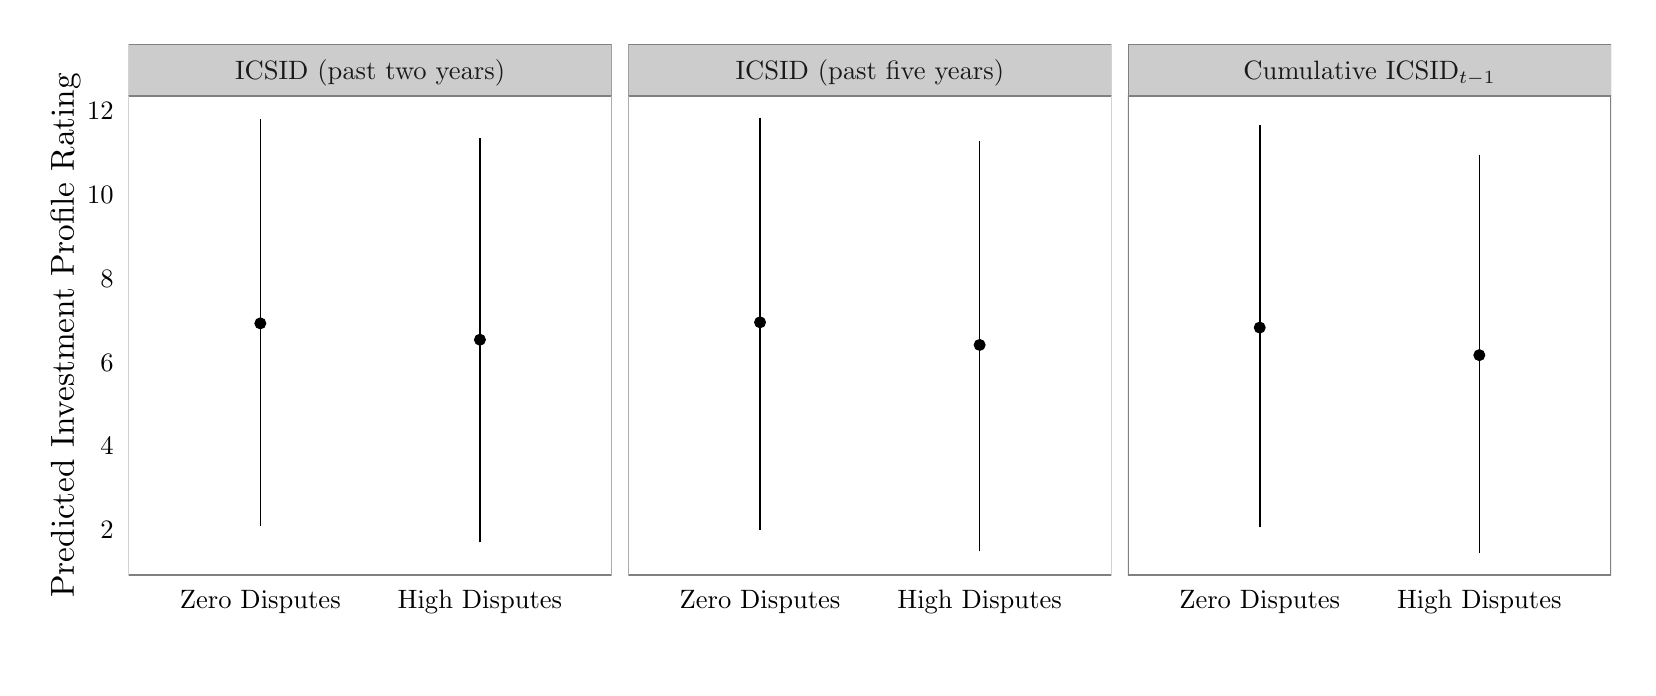
\begin{tikzpicture}[x=1pt,y=1pt]
\definecolor[named]{drawColor}{rgb}{0.00,0.00,0.00}
\definecolor[named]{fillColor}{rgb}{1.00,1.00,1.00}
\fill[color=fillColor,] (0,0) rectangle (578.16,231.26);
\begin{scope}
\path[clip] (  0.00,  0.00) rectangle (578.16,231.26);
\end{scope}
\begin{scope}
\path[clip] (  0.00,  0.00) rectangle (578.16,231.26);
\end{scope}
\begin{scope}
\path[clip] (  0.00,  0.00) rectangle (578.16,231.26);
\end{scope}
\begin{scope}
\path[clip] (  0.00,  0.00) rectangle (578.16,231.26);
\end{scope}
\begin{scope}
\path[clip] (  0.00,  0.00) rectangle (578.16,231.26);
\end{scope}
\begin{scope}
\path[clip] (  0.00,  0.00) rectangle (578.16,231.26);
\end{scope}
\begin{scope}
\path[clip] (  0.00,  0.00) rectangle (578.16,231.26);
\end{scope}
\begin{scope}
\path[clip] (  0.00,  0.00) rectangle (578.16,231.26);
\end{scope}
\begin{scope}
\path[clip] (  0.00,  0.00) rectangle (578.16,231.26);
\end{scope}
\begin{scope}
\path[clip] (  0.00,  0.00) rectangle (578.16,231.26);
\end{scope}
\begin{scope}
\path[clip] (  0.00,  0.00) rectangle (578.16,231.26);
\end{scope}
\begin{scope}
\path[clip] (  0.00,  0.00) rectangle (578.16,231.26);
\end{scope}
\begin{scope}
\path[clip] (  0.00,  0.00) rectangle (578.16,231.26);
\end{scope}
\begin{scope}
\path[clip] (  0.00,  0.00) rectangle (578.16,231.26);
\definecolor[named]{drawColor}{rgb}{1.00,1.00,1.00}
\definecolor[named]{fillColor}{rgb}{1.00,1.00,1.00}

\draw[color=drawColor,line width= 0.6pt,line cap=round,line join=round,fill=fillColor,] (  0.00,  0.00) rectangle (578.16,231.26);
\end{scope}
\begin{scope}
\path[clip] (  0.00,  0.00) rectangle (578.16,231.26);
\end{scope}
\begin{scope}
\path[clip] ( 36.46, 33.48) rectangle (211.03,206.65);
\definecolor[named]{fillColor}{rgb}{1.00,1.00,1.00}

\draw[fill=fillColor,draw opacity=0.00,] ( 36.46, 33.48) rectangle (211.03,206.65);
\definecolor[named]{drawColor}{rgb}{0.00,0.00,0.00}
\definecolor[named]{fillColor}{rgb}{0.00,0.00,0.00}

\draw[color=drawColor,line width= 0.6pt,line join=round,fill=fillColor,] ( 84.07, 51.23) -- ( 84.07,198.22);

\draw[color=drawColor,line width= 0.6pt,line join=round,fill=fillColor,] (163.42, 45.31) -- (163.42,191.56);

\draw[color=drawColor,line width= 0.4pt,line cap=round,line join=round,fill=fillColor,] ( 84.07,124.41) circle (  1.96);

\draw[color=drawColor,line width= 0.4pt,line cap=round,line join=round,fill=fillColor,] (163.42,118.50) circle (  1.96);
\definecolor[named]{drawColor}{rgb}{0.50,0.50,0.50}

\draw[color=drawColor,line width= 0.6pt,line cap=round,line join=round,fill opacity=0.00,] ( 36.46, 33.48) rectangle (211.03,206.65);
\end{scope}
\begin{scope}
\path[clip] (  0.00,  0.00) rectangle (578.16,231.26);
\end{scope}
\begin{scope}
\path[clip] (217.03, 33.48) rectangle (391.59,206.65);
\definecolor[named]{fillColor}{rgb}{1.00,1.00,1.00}

\draw[fill=fillColor,draw opacity=0.00,] (217.03, 33.48) rectangle (391.59,206.65);
\definecolor[named]{drawColor}{rgb}{0.00,0.00,0.00}
\definecolor[named]{fillColor}{rgb}{0.00,0.00,0.00}

\draw[color=drawColor,line width= 0.6pt,line join=round,fill=fillColor,] (264.64, 49.75) -- (264.64,198.78);

\draw[color=drawColor,line width= 0.6pt,line join=round,fill=fillColor,] (343.99, 42.06) -- (343.99,190.16);

\draw[color=drawColor,line width= 0.4pt,line cap=round,line join=round,fill=fillColor,] (264.64,124.79) circle (  1.96);

\draw[color=drawColor,line width= 0.4pt,line cap=round,line join=round,fill=fillColor,] (343.99,116.61) circle (  1.96);
\definecolor[named]{drawColor}{rgb}{0.50,0.50,0.50}

\draw[color=drawColor,line width= 0.6pt,line cap=round,line join=round,fill opacity=0.00,] (217.03, 33.48) rectangle (391.59,206.65);
\end{scope}
\begin{scope}
\path[clip] (  0.00,  0.00) rectangle (578.16,231.26);
\end{scope}
\begin{scope}
\path[clip] (397.59, 33.48) rectangle (572.16,206.65);
\definecolor[named]{fillColor}{rgb}{1.00,1.00,1.00}

\draw[fill=fillColor,draw opacity=0.00,] (397.59, 33.48) rectangle (572.16,206.65);
\definecolor[named]{drawColor}{rgb}{0.00,0.00,0.00}
\definecolor[named]{fillColor}{rgb}{0.00,0.00,0.00}

\draw[color=drawColor,line width= 0.6pt,line join=round,fill=fillColor,] (445.20, 50.70) -- (445.20,196.03);

\draw[color=drawColor,line width= 0.6pt,line join=round,fill=fillColor,] (524.55, 41.35) -- (524.55,185.34);

\draw[color=drawColor,line width= 0.4pt,line cap=round,line join=round,fill=fillColor,] (445.20,122.89) circle (  1.96);

\draw[color=drawColor,line width= 0.4pt,line cap=round,line join=round,fill=fillColor,] (524.55,112.93) circle (  1.96);
\definecolor[named]{drawColor}{rgb}{0.50,0.50,0.50}

\draw[color=drawColor,line width= 0.6pt,line cap=round,line join=round,fill opacity=0.00,] (397.59, 33.48) rectangle (572.16,206.65);
\end{scope}
\begin{scope}
\path[clip] (  0.00,  0.00) rectangle (578.16,231.26);
\end{scope}
\begin{scope}
\path[clip] (  0.00,  0.00) rectangle (578.16,231.26);
\end{scope}
\begin{scope}
\path[clip] (  0.00,  0.00) rectangle (578.16,231.26);
\end{scope}
\begin{scope}
\path[clip] ( 36.46,206.65) rectangle (211.03,225.26);
\definecolor[named]{drawColor}{rgb}{0.50,0.50,0.50}
\definecolor[named]{fillColor}{rgb}{0.80,0.80,0.80}

\draw[color=drawColor,line width= 0.2pt,line cap=round,line join=round,fill=fillColor,] ( 36.46,206.65) rectangle (211.03,225.26);
\definecolor[named]{drawColor}{rgb}{0.10,0.10,0.10}

\node[color=drawColor,anchor=base,inner sep=0pt, outer sep=0pt, scale=  0.96] at (123.75,212.65) {ICSID (past two years)%
};
\end{scope}
\begin{scope}
\path[clip] ( 36.46,206.65) rectangle (211.03,225.26);
\end{scope}
\begin{scope}
\path[clip] (  0.00,  0.00) rectangle (578.16,231.26);
\end{scope}
\begin{scope}
\path[clip] (  0.00,  0.00) rectangle (578.16,231.26);
\end{scope}
\begin{scope}
\path[clip] (  0.00,  0.00) rectangle (578.16,231.26);
\end{scope}
\begin{scope}
\path[clip] (  0.00,  0.00) rectangle (578.16,231.26);
\end{scope}
\begin{scope}
\path[clip] (  0.00,  0.00) rectangle (578.16,231.26);
\end{scope}
\begin{scope}
\path[clip] (  0.00,  0.00) rectangle (578.16,231.26);
\end{scope}
\begin{scope}
\path[clip] (217.03,206.65) rectangle (391.59,225.26);
\definecolor[named]{drawColor}{rgb}{0.50,0.50,0.50}
\definecolor[named]{fillColor}{rgb}{0.80,0.80,0.80}

\draw[color=drawColor,line width= 0.2pt,line cap=round,line join=round,fill=fillColor,] (217.03,206.65) rectangle (391.59,225.26);
\definecolor[named]{drawColor}{rgb}{0.10,0.10,0.10}

\node[color=drawColor,anchor=base,inner sep=0pt, outer sep=0pt, scale=  0.96] at (304.31,212.65) {ICSID (past five years)%
};
\end{scope}
\begin{scope}
\path[clip] (217.03,206.65) rectangle (391.59,225.26);
\end{scope}
\begin{scope}
\path[clip] (  0.00,  0.00) rectangle (578.16,231.26);
\end{scope}
\begin{scope}
\path[clip] (  0.00,  0.00) rectangle (578.16,231.26);
\end{scope}
\begin{scope}
\path[clip] (  0.00,  0.00) rectangle (578.16,231.26);
\end{scope}
\begin{scope}
\path[clip] (  0.00,  0.00) rectangle (578.16,231.26);
\end{scope}
\begin{scope}
\path[clip] (  0.00,  0.00) rectangle (578.16,231.26);
\end{scope}
\begin{scope}
\path[clip] (  0.00,  0.00) rectangle (578.16,231.26);
\end{scope}
\begin{scope}
\path[clip] (397.59,206.65) rectangle (572.16,225.26);
\definecolor[named]{drawColor}{rgb}{0.50,0.50,0.50}
\definecolor[named]{fillColor}{rgb}{0.80,0.80,0.80}

\draw[color=drawColor,line width= 0.2pt,line cap=round,line join=round,fill=fillColor,] (397.59,206.65) rectangle (572.16,225.26);
\definecolor[named]{drawColor}{rgb}{0.10,0.10,0.10}

\node[color=drawColor,anchor=base,inner sep=0pt, outer sep=0pt, scale=  0.96] at (484.88,212.65) {Cumulative ICSID$_{t-1}$%
};
\end{scope}
\begin{scope}
\path[clip] (397.59,206.65) rectangle (572.16,225.26);
\end{scope}
\begin{scope}
\path[clip] (  0.00,  0.00) rectangle (578.16,231.26);
\end{scope}
\begin{scope}
\path[clip] (  0.00,  0.00) rectangle (578.16,231.26);
\end{scope}
\begin{scope}
\path[clip] (  0.00,  0.00) rectangle (578.16,231.26);
\end{scope}
\begin{scope}
\path[clip] (  0.00,  0.00) rectangle (578.16,231.26);
\end{scope}
\begin{scope}
\path[clip] (  0.00,  0.00) rectangle (578.16,231.26);
\end{scope}
\begin{scope}
\path[clip] (  0.00,  0.00) rectangle (578.16,231.26);
\end{scope}
\begin{scope}
\path[clip] (  0.00,  0.00) rectangle (578.16,231.26);
\end{scope}
\begin{scope}
\path[clip] (  0.00,  0.00) rectangle (578.16,231.26);
\end{scope}
\begin{scope}
\path[clip] (  0.00,  0.00) rectangle (578.16,231.26);
\definecolor[named]{drawColor}{rgb}{0.00,0.00,0.00}

\node[color=drawColor,anchor=base east,inner sep=0pt, outer sep=0pt, scale=  0.96] at ( 31.06, 46.57) {2%
};

\node[color=drawColor,anchor=base east,inner sep=0pt, outer sep=0pt, scale=  0.96] at ( 31.06, 76.85) {4%
};

\node[color=drawColor,anchor=base east,inner sep=0pt, outer sep=0pt, scale=  0.96] at ( 31.06,107.14) {6%
};

\node[color=drawColor,anchor=base east,inner sep=0pt, outer sep=0pt, scale=  0.96] at ( 31.06,137.42) {8%
};

\node[color=drawColor,anchor=base east,inner sep=0pt, outer sep=0pt, scale=  0.96] at ( 31.06,167.70) {10%
};

\node[color=drawColor,anchor=base east,inner sep=0pt, outer sep=0pt, scale=  0.96] at ( 31.06,197.98) {12%
};
\end{scope}
\begin{scope}
\path[clip] (  0.00,  0.00) rectangle (578.16,231.26);
\end{scope}
\begin{scope}
\path[clip] (  0.00,  0.00) rectangle (578.16,231.26);
\end{scope}
\begin{scope}
\path[clip] (  0.00,  0.00) rectangle (578.16,231.26);
\end{scope}
\begin{scope}
\path[clip] (  0.00,  0.00) rectangle (578.16,231.26);
\end{scope}
\begin{scope}
\path[clip] (  0.00,  0.00) rectangle (578.16,231.26);
\end{scope}
\begin{scope}
\path[clip] (  0.00,  0.00) rectangle (578.16,231.26);
\end{scope}
\begin{scope}
\path[clip] (  0.00,  0.00) rectangle (578.16,231.26);
\end{scope}
\begin{scope}
\path[clip] (  0.00,  0.00) rectangle (578.16,231.26);
\end{scope}
\begin{scope}
\path[clip] (  0.00,  0.00) rectangle (578.16,231.26);
\end{scope}
\begin{scope}
\path[clip] (  0.00,  0.00) rectangle (578.16,231.26);
\end{scope}
\begin{scope}
\path[clip] (  0.00,  0.00) rectangle (578.16,231.26);
\end{scope}
\begin{scope}
\path[clip] (  0.00,  0.00) rectangle (578.16,231.26);
\end{scope}
\begin{scope}
\path[clip] (  0.00,  0.00) rectangle (578.16,231.26);
\end{scope}
\begin{scope}
\path[clip] (  0.00,  0.00) rectangle (578.16,231.26);
\end{scope}
\begin{scope}
\path[clip] (  0.00,  0.00) rectangle (578.16,231.26);
\end{scope}
\begin{scope}
\path[clip] (  0.00,  0.00) rectangle (578.16,231.26);
\end{scope}
\begin{scope}
\path[clip] (  0.00,  0.00) rectangle (578.16,231.26);
\end{scope}
\begin{scope}
\path[clip] (  0.00,  0.00) rectangle (578.16,231.26);
\definecolor[named]{drawColor}{rgb}{0.00,0.00,0.00}

\node[color=drawColor,anchor=base,inner sep=0pt, outer sep=0pt, scale=  0.96] at ( 84.07, 21.46) {Zero Disputes%
};

\node[color=drawColor,anchor=base,inner sep=0pt, outer sep=0pt, scale=  0.96] at (163.42, 21.46) {High Disputes%
};
\end{scope}
\begin{scope}
\path[clip] (  0.00,  0.00) rectangle (578.16,231.26);
\end{scope}
\begin{scope}
\path[clip] (  0.00,  0.00) rectangle (578.16,231.26);
\end{scope}
\begin{scope}
\path[clip] (  0.00,  0.00) rectangle (578.16,231.26);
\end{scope}
\begin{scope}
\path[clip] (  0.00,  0.00) rectangle (578.16,231.26);
\end{scope}
\begin{scope}
\path[clip] (  0.00,  0.00) rectangle (578.16,231.26);
\end{scope}
\begin{scope}
\path[clip] (  0.00,  0.00) rectangle (578.16,231.26);
\end{scope}
\begin{scope}
\path[clip] (  0.00,  0.00) rectangle (578.16,231.26);
\end{scope}
\begin{scope}
\path[clip] (  0.00,  0.00) rectangle (578.16,231.26);
\end{scope}
\begin{scope}
\path[clip] (  0.00,  0.00) rectangle (578.16,231.26);
\end{scope}
\begin{scope}
\path[clip] (  0.00,  0.00) rectangle (578.16,231.26);
\end{scope}
\begin{scope}
\path[clip] (  0.00,  0.00) rectangle (578.16,231.26);
\end{scope}
\begin{scope}
\path[clip] (  0.00,  0.00) rectangle (578.16,231.26);
\definecolor[named]{drawColor}{rgb}{0.00,0.00,0.00}

\node[color=drawColor,anchor=base,inner sep=0pt, outer sep=0pt, scale=  0.96] at (264.64, 21.46) {Zero Disputes%
};

\node[color=drawColor,anchor=base,inner sep=0pt, outer sep=0pt, scale=  0.96] at (343.99, 21.46) {High Disputes%
};
\end{scope}
\begin{scope}
\path[clip] (  0.00,  0.00) rectangle (578.16,231.26);
\end{scope}
\begin{scope}
\path[clip] (  0.00,  0.00) rectangle (578.16,231.26);
\end{scope}
\begin{scope}
\path[clip] (  0.00,  0.00) rectangle (578.16,231.26);
\end{scope}
\begin{scope}
\path[clip] (  0.00,  0.00) rectangle (578.16,231.26);
\end{scope}
\begin{scope}
\path[clip] (  0.00,  0.00) rectangle (578.16,231.26);
\end{scope}
\begin{scope}
\path[clip] (  0.00,  0.00) rectangle (578.16,231.26);
\end{scope}
\begin{scope}
\path[clip] (  0.00,  0.00) rectangle (578.16,231.26);
\end{scope}
\begin{scope}
\path[clip] (  0.00,  0.00) rectangle (578.16,231.26);
\end{scope}
\begin{scope}
\path[clip] (  0.00,  0.00) rectangle (578.16,231.26);
\end{scope}
\begin{scope}
\path[clip] (  0.00,  0.00) rectangle (578.16,231.26);
\end{scope}
\begin{scope}
\path[clip] (  0.00,  0.00) rectangle (578.16,231.26);
\end{scope}
\begin{scope}
\path[clip] (  0.00,  0.00) rectangle (578.16,231.26);
\definecolor[named]{drawColor}{rgb}{0.00,0.00,0.00}

\node[color=drawColor,anchor=base,inner sep=0pt, outer sep=0pt, scale=  0.96] at (445.20, 21.46) {Zero Disputes%
};

\node[color=drawColor,anchor=base,inner sep=0pt, outer sep=0pt, scale=  0.96] at (524.55, 21.46) {High Disputes%
};
\end{scope}
\begin{scope}
\path[clip] (  0.00,  0.00) rectangle (578.16,231.26);
\end{scope}
\begin{scope}
\path[clip] (  0.00,  0.00) rectangle (578.16,231.26);
\end{scope}
\begin{scope}
\path[clip] (  0.00,  0.00) rectangle (578.16,231.26);
\end{scope}
\begin{scope}
\path[clip] (  0.00,  0.00) rectangle (578.16,231.26);
\end{scope}
\begin{scope}
\path[clip] (  0.00,  0.00) rectangle (578.16,231.26);
\end{scope}
\begin{scope}
\path[clip] (  0.00,  0.00) rectangle (578.16,231.26);
\end{scope}
\begin{scope}
\path[clip] (  0.00,  0.00) rectangle (578.16,231.26);
\end{scope}
\begin{scope}
\path[clip] (  0.00,  0.00) rectangle (578.16,231.26);
\end{scope}
\begin{scope}
\path[clip] (  0.00,  0.00) rectangle (578.16,231.26);
\definecolor[named]{drawColor}{rgb}{0.00,0.00,0.00}

\node[rotate= 90.00,color=drawColor,anchor=base,inner sep=0pt, outer sep=0pt, scale=  1.20] at ( 16.66,120.06) {Predicted Investment Profile Rating%
};
\end{scope}
\begin{scope}
\path[clip] (  0.00,  0.00) rectangle (578.16,231.26);
\end{scope}
\begin{scope}
\path[clip] (  0.00,  0.00) rectangle (578.16,231.26);
\end{scope}
\begin{scope}
\path[clip] (  0.00,  0.00) rectangle (578.16,231.26);
\end{scope}
\begin{scope}
\path[clip] (  0.00,  0.00) rectangle (578.16,231.26);
\end{scope}
\begin{scope}
\path[clip] (  0.00,  0.00) rectangle (578.16,231.26);
\end{scope}
\end{tikzpicture}
}	
\end{figure}

\end{frame}
%%%%%%%%%%%%%%%%%%%%%%%%%%%%%%%%%%%%%%%%%

%%%%%%%%%%%%%%%%%%%%%%%%%%%%%%%%%%%%%%%%%
\begin{frame}
\frametitle{Change over Disputes Over Time}

% \pause
\begin{figure}[ht]
	\centering
	\resizebox{1\textwidth}{!}{% Created by tikzDevice version 0.7.0 on 2015-01-17 17:55:38
% !TEX encoding = UTF-8 Unicode
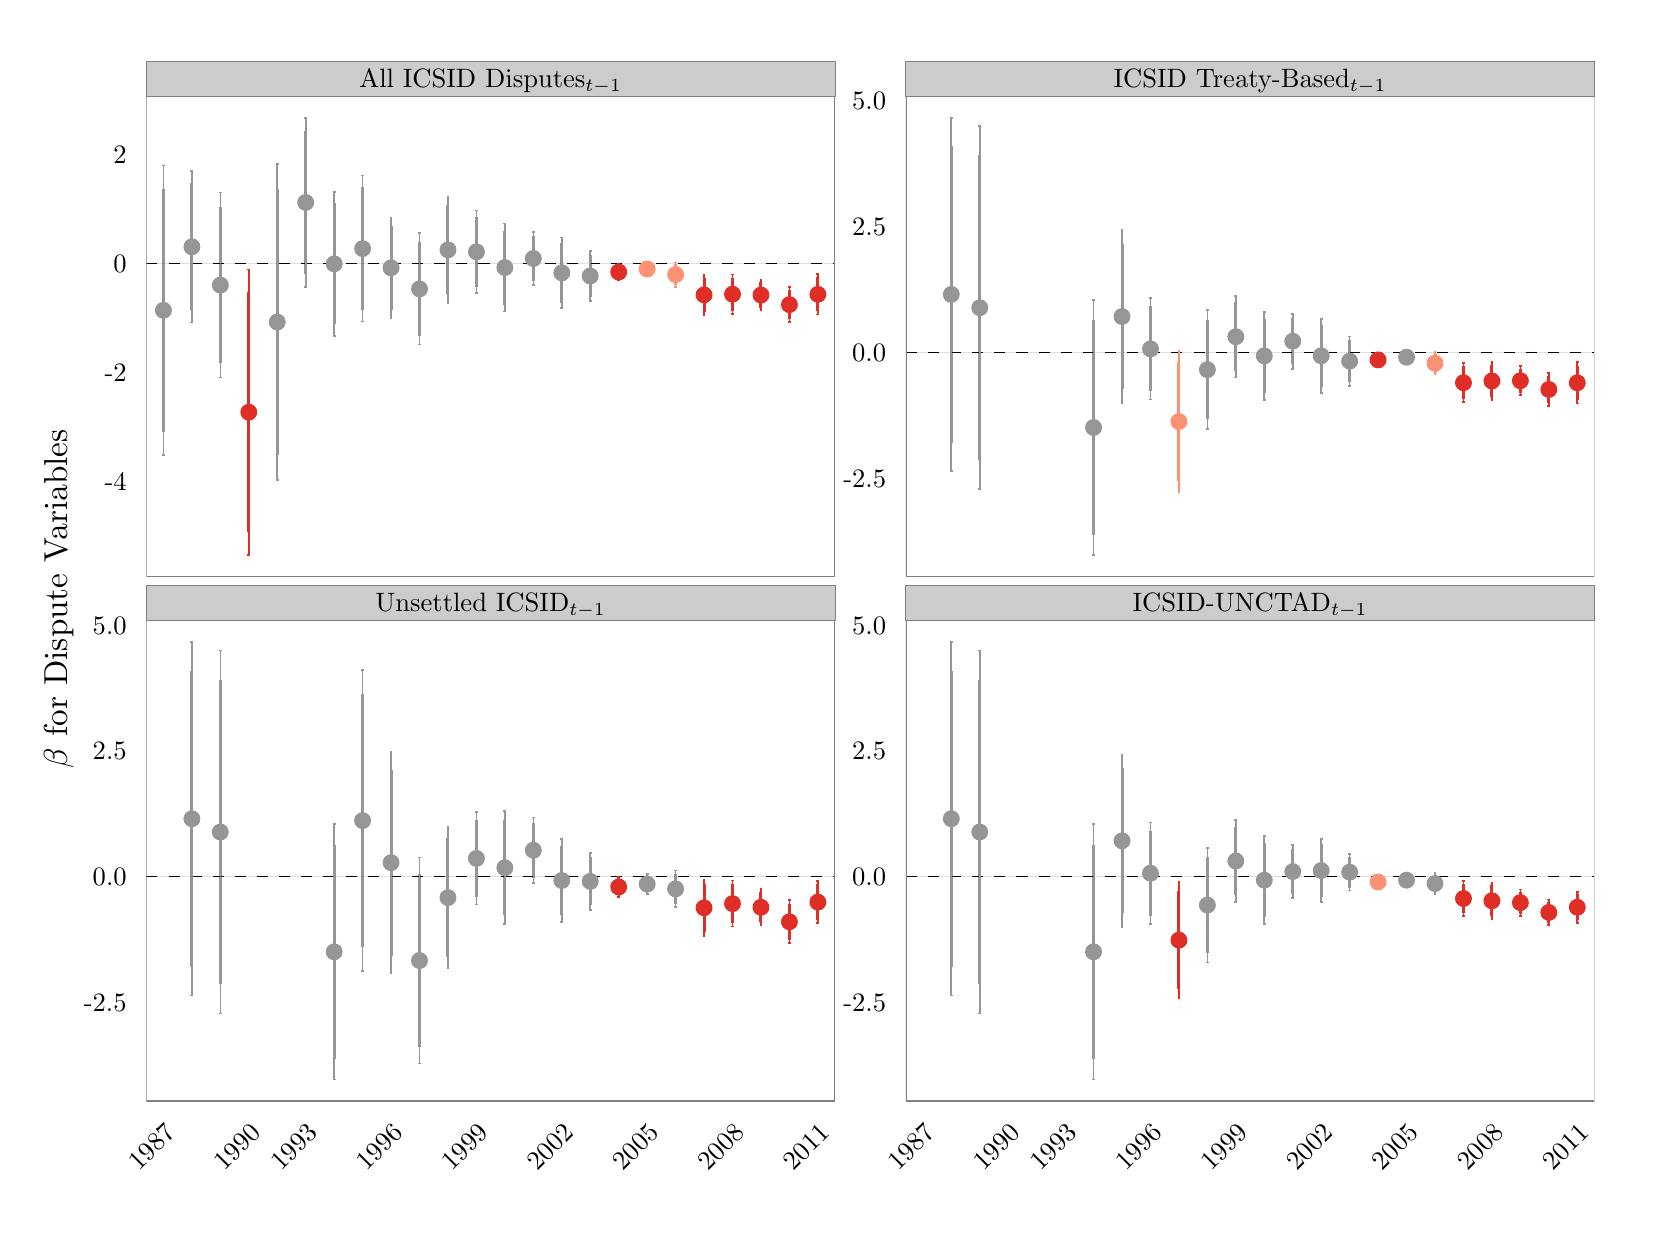
\begin{tikzpicture}[x=1pt,y=1pt]
\definecolor[named]{fillColor}{rgb}{1.00,1.00,1.00}
\path[use as bounding box,fill=fillColor,fill opacity=0.00] (0,0) rectangle (578.16,433.62);
\begin{scope}
\path[clip] (  0.00,  0.00) rectangle (578.16,433.62);
\definecolor[named]{drawColor}{rgb}{1.00,1.00,1.00}
\definecolor[named]{fillColor}{rgb}{1.00,1.00,1.00}

\path[draw=drawColor,line width= 0.6pt,line join=round,line cap=round,fill=fillColor] (  0.00,  0.00) rectangle (578.16,433.62);
\end{scope}
\begin{scope}
\path[clip] ( 42.89,235.13) rectangle (291.71,408.94);
\definecolor[named]{fillColor}{rgb}{1.00,1.00,1.00}

\path[fill=fillColor] ( 42.89,235.13) rectangle (291.71,408.94);
\definecolor[named]{drawColor}{rgb}{0.59,0.59,0.59}
\definecolor[named]{fillColor}{rgb}{0.59,0.59,0.59}

\path[draw=drawColor,draw opacity=0.30,line width= 0.3pt,line join=round,fill=fillColor,fill opacity=0.30] ( 49.05,279.17) -- ( 49.05,383.79);

\path[draw=drawColor,draw opacity=0.30,line width= 0.3pt,line join=round,fill=fillColor,fill opacity=0.30] ( 59.34,327.06) -- ( 59.34,381.80);

\path[draw=drawColor,draw opacity=0.30,line width= 0.3pt,line join=round,fill=fillColor,fill opacity=0.30] ( 69.62,307.18) -- ( 69.62,374.02);
\definecolor[named]{drawColor}{rgb}{0.87,0.18,0.15}
\definecolor[named]{fillColor}{rgb}{0.87,0.18,0.15}

\path[draw=drawColor,draw opacity=0.30,line width= 0.3pt,line join=round,fill=fillColor,fill opacity=0.30] ( 79.90,243.03) -- ( 79.90,346.28);
\definecolor[named]{drawColor}{rgb}{0.59,0.59,0.59}
\definecolor[named]{fillColor}{rgb}{0.59,0.59,0.59}

\path[draw=drawColor,draw opacity=0.30,line width= 0.3pt,line join=round,fill=fillColor,fill opacity=0.30] ( 90.18,270.12) -- ( 90.18,384.39);

\path[draw=drawColor,draw opacity=0.30,line width= 0.3pt,line join=round,fill=fillColor,fill opacity=0.30] (100.46,339.87) -- (100.46,401.04);

\path[draw=drawColor,draw opacity=0.30,line width= 0.3pt,line join=round,fill=fillColor,fill opacity=0.30] (110.75,322.30) -- (110.75,374.27);

\path[draw=drawColor,draw opacity=0.30,line width= 0.3pt,line join=round,fill=fillColor,fill opacity=0.30] (121.03,327.40) -- (121.03,380.17);

\path[draw=drawColor,draw opacity=0.30,line width= 0.3pt,line join=round,fill=fillColor,fill opacity=0.30] (131.31,328.76) -- (131.31,364.94);

\path[draw=drawColor,draw opacity=0.30,line width= 0.3pt,line join=round,fill=fillColor,fill opacity=0.30] (141.59,319.07) -- (141.59,359.35);

\path[draw=drawColor,draw opacity=0.30,line width= 0.3pt,line join=round,fill=fillColor,fill opacity=0.30] (151.87,334.15) -- (151.87,372.51);

\path[draw=drawColor,draw opacity=0.30,line width= 0.3pt,line join=round,fill=fillColor,fill opacity=0.30] (162.16,337.67) -- (162.16,367.57);

\path[draw=drawColor,draw opacity=0.30,line width= 0.3pt,line join=round,fill=fillColor,fill opacity=0.30] (172.44,331.01) -- (172.44,362.86);

\path[draw=drawColor,draw opacity=0.30,line width= 0.3pt,line join=round,fill=fillColor,fill opacity=0.30] (182.72,340.60) -- (182.72,359.82);

\path[draw=drawColor,draw opacity=0.30,line width= 0.3pt,line join=round,fill=fillColor,fill opacity=0.30] (193.00,332.20) -- (193.00,357.84);

\path[draw=drawColor,draw opacity=0.30,line width= 0.3pt,line join=round,fill=fillColor,fill opacity=0.30] (203.28,334.77) -- (203.28,352.99);
\definecolor[named]{drawColor}{rgb}{0.87,0.18,0.15}
\definecolor[named]{fillColor}{rgb}{0.87,0.18,0.15}

\path[draw=drawColor,draw opacity=0.30,line width= 0.3pt,line join=round,fill=fillColor,fill opacity=0.30] (213.56,342.52) -- (213.56,348.12);
\definecolor[named]{drawColor}{rgb}{0.99,0.57,0.45}
\definecolor[named]{fillColor}{rgb}{0.99,0.57,0.45}

\path[draw=drawColor,draw opacity=0.30,line width= 0.3pt,line join=round,fill=fillColor,fill opacity=0.30] (223.85,344.07) -- (223.85,348.80);

\path[draw=drawColor,draw opacity=0.30,line width= 0.3pt,line join=round,fill=fillColor,fill opacity=0.30] (234.13,339.99) -- (234.13,348.81);
\definecolor[named]{drawColor}{rgb}{0.87,0.18,0.15}
\definecolor[named]{fillColor}{rgb}{0.87,0.18,0.15}

\path[draw=drawColor,draw opacity=0.30,line width= 0.3pt,line join=round,fill=fillColor,fill opacity=0.30] (244.41,329.66) -- (244.41,344.47);

\path[draw=drawColor,draw opacity=0.30,line width= 0.3pt,line join=round,fill=fillColor,fill opacity=0.30] (254.69,330.17) -- (254.69,344.45);

\path[draw=drawColor,draw opacity=0.30,line width= 0.3pt,line join=round,fill=fillColor,fill opacity=0.30] (264.97,331.37) -- (264.97,342.62);

\path[draw=drawColor,draw opacity=0.30,line width= 0.3pt,line join=round,fill=fillColor,fill opacity=0.30] (275.26,327.22) -- (275.26,339.84);

\path[draw=drawColor,draw opacity=0.30,line width= 0.3pt,line join=round,fill=fillColor,fill opacity=0.30] (285.54,329.97) -- (285.54,344.55);
\definecolor[named]{drawColor}{rgb}{0.59,0.59,0.59}
\definecolor[named]{fillColor}{rgb}{0.59,0.59,0.59}

\path[draw=drawColor,line width= 1.1pt,line join=round,fill=fillColor] ( 49.05,287.58) -- ( 49.05,375.38);

\path[draw=drawColor,line width= 1.1pt,line join=round,fill=fillColor] ( 59.34,331.46) -- ( 59.34,377.40);

\path[draw=drawColor,line width= 1.1pt,line join=round,fill=fillColor] ( 69.62,312.55) -- ( 69.62,368.65);
\definecolor[named]{drawColor}{rgb}{0.87,0.18,0.15}
\definecolor[named]{fillColor}{rgb}{0.87,0.18,0.15}

\path[draw=drawColor,line width= 1.1pt,line join=round,fill=fillColor] ( 79.90,251.33) -- ( 79.90,337.98);
\definecolor[named]{drawColor}{rgb}{0.59,0.59,0.59}
\definecolor[named]{fillColor}{rgb}{0.59,0.59,0.59}

\path[draw=drawColor,line width= 1.1pt,line join=round,fill=fillColor] ( 90.18,279.30) -- ( 90.18,375.20);

\path[draw=drawColor,line width= 1.1pt,line join=round,fill=fillColor] (100.46,344.78) -- (100.46,396.12);

\path[draw=drawColor,line width= 1.1pt,line join=round,fill=fillColor] (110.75,326.48) -- (110.75,370.09);

\path[draw=drawColor,line width= 1.1pt,line join=round,fill=fillColor] (121.03,331.64) -- (121.03,375.93);

\path[draw=drawColor,line width= 1.1pt,line join=round,fill=fillColor] (131.31,331.67) -- (131.31,362.03);

\path[draw=drawColor,line width= 1.1pt,line join=round,fill=fillColor] (141.59,322.31) -- (141.59,356.11);

\path[draw=drawColor,line width= 1.1pt,line join=round,fill=fillColor] (151.87,337.23) -- (151.87,369.43);

\path[draw=drawColor,line width= 1.1pt,line join=round,fill=fillColor] (162.16,340.07) -- (162.16,365.17);

\path[draw=drawColor,line width= 1.1pt,line join=round,fill=fillColor] (172.44,333.57) -- (172.44,360.30);

\path[draw=drawColor,line width= 1.1pt,line join=round,fill=fillColor] (182.72,342.14) -- (182.72,358.27);

\path[draw=drawColor,line width= 1.1pt,line join=round,fill=fillColor] (193.00,334.26) -- (193.00,355.78);

\path[draw=drawColor,line width= 1.1pt,line join=round,fill=fillColor] (203.28,336.24) -- (203.28,351.52);
\definecolor[named]{drawColor}{rgb}{0.87,0.18,0.15}
\definecolor[named]{fillColor}{rgb}{0.87,0.18,0.15}

\path[draw=drawColor,line width= 1.1pt,line join=round,fill=fillColor] (213.56,342.97) -- (213.56,347.67);
\definecolor[named]{drawColor}{rgb}{0.99,0.57,0.45}
\definecolor[named]{fillColor}{rgb}{0.99,0.57,0.45}

\path[draw=drawColor,line width= 1.1pt,line join=round,fill=fillColor] (223.85,344.45) -- (223.85,348.42);

\path[draw=drawColor,line width= 1.1pt,line join=round,fill=fillColor] (234.13,340.70) -- (234.13,348.10);
\definecolor[named]{drawColor}{rgb}{0.87,0.18,0.15}
\definecolor[named]{fillColor}{rgb}{0.87,0.18,0.15}

\path[draw=drawColor,line width= 1.1pt,line join=round,fill=fillColor] (244.41,330.85) -- (244.41,343.28);

\path[draw=drawColor,line width= 1.1pt,line join=round,fill=fillColor] (254.69,331.32) -- (254.69,343.30);

\path[draw=drawColor,line width= 1.1pt,line join=round,fill=fillColor] (264.97,332.28) -- (264.97,341.71);

\path[draw=drawColor,line width= 1.1pt,line join=round,fill=fillColor] (275.26,328.24) -- (275.26,338.83);

\path[draw=drawColor,line width= 1.1pt,line join=round,fill=fillColor] (285.54,331.14) -- (285.54,343.38);
\definecolor[named]{drawColor}{rgb}{0.00,0.00,0.00}
\definecolor[named]{fillColor}{rgb}{0.00,0.00,0.00}

\path[draw=drawColor,line width= 0.6pt,dash pattern=on 4pt off 4pt ,line join=round,fill=fillColor] ( 42.89,348.44) -- (291.71,348.44);
\definecolor[named]{drawColor}{rgb}{0.59,0.59,0.59}
\definecolor[named]{fillColor}{rgb}{0.59,0.59,0.59}

\path[draw=drawColor,line width= 0.4pt,line join=round,line cap=round,fill=fillColor] ( 49.05,331.48) circle (  2.85);

\path[draw=drawColor,line width= 0.4pt,line join=round,line cap=round,fill=fillColor] ( 59.34,354.43) circle (  2.85);

\path[draw=drawColor,line width= 0.4pt,line join=round,line cap=round,fill=fillColor] ( 69.62,340.60) circle (  2.85);
\definecolor[named]{drawColor}{rgb}{0.87,0.18,0.15}
\definecolor[named]{fillColor}{rgb}{0.87,0.18,0.15}

\path[draw=drawColor,line width= 0.4pt,line join=round,line cap=round,fill=fillColor] ( 79.90,294.66) circle (  2.85);
\definecolor[named]{drawColor}{rgb}{0.59,0.59,0.59}
\definecolor[named]{fillColor}{rgb}{0.59,0.59,0.59}

\path[draw=drawColor,line width= 0.4pt,line join=round,line cap=round,fill=fillColor] ( 90.18,327.25) circle (  2.85);

\path[draw=drawColor,line width= 0.4pt,line join=round,line cap=round,fill=fillColor] (100.46,370.45) circle (  2.85);

\path[draw=drawColor,line width= 0.4pt,line join=round,line cap=round,fill=fillColor] (110.75,348.28) circle (  2.85);

\path[draw=drawColor,line width= 0.4pt,line join=round,line cap=round,fill=fillColor] (121.03,353.79) circle (  2.85);

\path[draw=drawColor,line width= 0.4pt,line join=round,line cap=round,fill=fillColor] (131.31,346.85) circle (  2.85);

\path[draw=drawColor,line width= 0.4pt,line join=round,line cap=round,fill=fillColor] (141.59,339.21) circle (  2.85);

\path[draw=drawColor,line width= 0.4pt,line join=round,line cap=round,fill=fillColor] (151.87,353.33) circle (  2.85);

\path[draw=drawColor,line width= 0.4pt,line join=round,line cap=round,fill=fillColor] (162.16,352.62) circle (  2.85);

\path[draw=drawColor,line width= 0.4pt,line join=round,line cap=round,fill=fillColor] (172.44,346.94) circle (  2.85);

\path[draw=drawColor,line width= 0.4pt,line join=round,line cap=round,fill=fillColor] (182.72,350.21) circle (  2.85);

\path[draw=drawColor,line width= 0.4pt,line join=round,line cap=round,fill=fillColor] (193.00,345.02) circle (  2.85);

\path[draw=drawColor,line width= 0.4pt,line join=round,line cap=round,fill=fillColor] (203.28,343.88) circle (  2.85);
\definecolor[named]{drawColor}{rgb}{0.87,0.18,0.15}
\definecolor[named]{fillColor}{rgb}{0.87,0.18,0.15}

\path[draw=drawColor,line width= 0.4pt,line join=round,line cap=round,fill=fillColor] (213.56,345.32) circle (  2.85);
\definecolor[named]{drawColor}{rgb}{0.99,0.57,0.45}
\definecolor[named]{fillColor}{rgb}{0.99,0.57,0.45}

\path[draw=drawColor,line width= 0.4pt,line join=round,line cap=round,fill=fillColor] (223.85,346.43) circle (  2.85);

\path[draw=drawColor,line width= 0.4pt,line join=round,line cap=round,fill=fillColor] (234.13,344.40) circle (  2.85);
\definecolor[named]{drawColor}{rgb}{0.87,0.18,0.15}
\definecolor[named]{fillColor}{rgb}{0.87,0.18,0.15}

\path[draw=drawColor,line width= 0.4pt,line join=round,line cap=round,fill=fillColor] (244.41,337.07) circle (  2.85);

\path[draw=drawColor,line width= 0.4pt,line join=round,line cap=round,fill=fillColor] (254.69,337.31) circle (  2.85);

\path[draw=drawColor,line width= 0.4pt,line join=round,line cap=round,fill=fillColor] (264.97,337.00) circle (  2.85);

\path[draw=drawColor,line width= 0.4pt,line join=round,line cap=round,fill=fillColor] (275.26,333.53) circle (  2.85);

\path[draw=drawColor,line width= 0.4pt,line join=round,line cap=round,fill=fillColor] (285.54,337.26) circle (  2.85);
\definecolor[named]{drawColor}{rgb}{0.59,0.59,0.59}

\path[draw=drawColor,line width= 0.6pt,line join=round] ( 48.54,383.79) --
	( 49.57,383.79);

\path[draw=drawColor,line width= 0.6pt,line join=round] ( 49.05,383.79) --
	( 49.05,279.17);

\path[draw=drawColor,line width= 0.6pt,line join=round] ( 48.54,279.17) --
	( 49.57,279.17);

\path[draw=drawColor,line width= 0.6pt,line join=round] ( 58.82,381.80) --
	( 59.85,381.80);

\path[draw=drawColor,line width= 0.6pt,line join=round] ( 59.34,381.80) --
	( 59.34,327.06);

\path[draw=drawColor,line width= 0.6pt,line join=round] ( 58.82,327.06) --
	( 59.85,327.06);

\path[draw=drawColor,line width= 0.6pt,line join=round] ( 69.10,374.02) --
	( 70.13,374.02);

\path[draw=drawColor,line width= 0.6pt,line join=round] ( 69.62,374.02) --
	( 69.62,307.18);

\path[draw=drawColor,line width= 0.6pt,line join=round] ( 69.10,307.18) --
	( 70.13,307.18);
\definecolor[named]{drawColor}{rgb}{0.87,0.18,0.15}

\path[draw=drawColor,line width= 0.6pt,line join=round] ( 79.39,346.28) --
	( 80.41,346.28);

\path[draw=drawColor,line width= 0.6pt,line join=round] ( 79.90,346.28) --
	( 79.90,243.03);

\path[draw=drawColor,line width= 0.6pt,line join=round] ( 79.39,243.03) --
	( 80.41,243.03);
\definecolor[named]{drawColor}{rgb}{0.59,0.59,0.59}

\path[draw=drawColor,line width= 0.6pt,line join=round] ( 89.67,384.39) --
	( 90.70,384.39);

\path[draw=drawColor,line width= 0.6pt,line join=round] ( 90.18,384.39) --
	( 90.18,270.12);

\path[draw=drawColor,line width= 0.6pt,line join=round] ( 89.67,270.12) --
	( 90.70,270.12);

\path[draw=drawColor,line width= 0.6pt,line join=round] ( 99.95,401.04) --
	(100.98,401.04);

\path[draw=drawColor,line width= 0.6pt,line join=round] (100.46,401.04) --
	(100.46,339.87);

\path[draw=drawColor,line width= 0.6pt,line join=round] ( 99.95,339.87) --
	(100.98,339.87);

\path[draw=drawColor,line width= 0.6pt,line join=round] (110.23,374.27) --
	(111.26,374.27);

\path[draw=drawColor,line width= 0.6pt,line join=round] (110.75,374.27) --
	(110.75,322.30);

\path[draw=drawColor,line width= 0.6pt,line join=round] (110.23,322.30) --
	(111.26,322.30);

\path[draw=drawColor,line width= 0.6pt,line join=round] (120.51,380.17) --
	(121.54,380.17);

\path[draw=drawColor,line width= 0.6pt,line join=round] (121.03,380.17) --
	(121.03,327.40);

\path[draw=drawColor,line width= 0.6pt,line join=round] (120.51,327.40) --
	(121.54,327.40);

\path[draw=drawColor,line width= 0.6pt,line join=round] (130.80,364.94) --
	(131.82,364.94);

\path[draw=drawColor,line width= 0.6pt,line join=round] (131.31,364.94) --
	(131.31,328.76);

\path[draw=drawColor,line width= 0.6pt,line join=round] (130.80,328.76) --
	(131.82,328.76);

\path[draw=drawColor,line width= 0.6pt,line join=round] (141.08,359.35) --
	(142.11,359.35);

\path[draw=drawColor,line width= 0.6pt,line join=round] (141.59,359.35) --
	(141.59,319.07);

\path[draw=drawColor,line width= 0.6pt,line join=round] (141.08,319.07) --
	(142.11,319.07);

\path[draw=drawColor,line width= 0.6pt,line join=round] (151.36,372.51) --
	(152.39,372.51);

\path[draw=drawColor,line width= 0.6pt,line join=round] (151.87,372.51) --
	(151.87,334.15);

\path[draw=drawColor,line width= 0.6pt,line join=round] (151.36,334.15) --
	(152.39,334.15);

\path[draw=drawColor,line width= 0.6pt,line join=round] (161.64,367.57) --
	(162.67,367.57);

\path[draw=drawColor,line width= 0.6pt,line join=round] (162.16,367.57) --
	(162.16,337.67);

\path[draw=drawColor,line width= 0.6pt,line join=round] (161.64,337.67) --
	(162.67,337.67);

\path[draw=drawColor,line width= 0.6pt,line join=round] (171.92,362.86) --
	(172.95,362.86);

\path[draw=drawColor,line width= 0.6pt,line join=round] (172.44,362.86) --
	(172.44,331.01);

\path[draw=drawColor,line width= 0.6pt,line join=round] (171.92,331.01) --
	(172.95,331.01);

\path[draw=drawColor,line width= 0.6pt,line join=round] (182.20,359.82) --
	(183.23,359.82);

\path[draw=drawColor,line width= 0.6pt,line join=round] (182.72,359.82) --
	(182.72,340.60);

\path[draw=drawColor,line width= 0.6pt,line join=round] (182.20,340.60) --
	(183.23,340.60);

\path[draw=drawColor,line width= 0.6pt,line join=round] (192.49,357.84) --
	(193.51,357.84);

\path[draw=drawColor,line width= 0.6pt,line join=round] (193.00,357.84) --
	(193.00,332.20);

\path[draw=drawColor,line width= 0.6pt,line join=round] (192.49,332.20) --
	(193.51,332.20);

\path[draw=drawColor,line width= 0.6pt,line join=round] (202.77,352.99) --
	(203.80,352.99);

\path[draw=drawColor,line width= 0.6pt,line join=round] (203.28,352.99) --
	(203.28,334.77);

\path[draw=drawColor,line width= 0.6pt,line join=round] (202.77,334.77) --
	(203.80,334.77);
\definecolor[named]{drawColor}{rgb}{0.87,0.18,0.15}

\path[draw=drawColor,line width= 0.6pt,line join=round] (213.05,348.12) --
	(214.08,348.12);

\path[draw=drawColor,line width= 0.6pt,line join=round] (213.56,348.12) --
	(213.56,342.52);

\path[draw=drawColor,line width= 0.6pt,line join=round] (213.05,342.52) --
	(214.08,342.52);
\definecolor[named]{drawColor}{rgb}{0.99,0.57,0.45}

\path[draw=drawColor,line width= 0.6pt,line join=round] (223.33,348.80) --
	(224.36,348.80);

\path[draw=drawColor,line width= 0.6pt,line join=round] (223.85,348.80) --
	(223.85,344.07);

\path[draw=drawColor,line width= 0.6pt,line join=round] (223.33,344.07) --
	(224.36,344.07);

\path[draw=drawColor,line width= 0.6pt,line join=round] (233.61,348.81) --
	(234.64,348.81);

\path[draw=drawColor,line width= 0.6pt,line join=round] (234.13,348.81) --
	(234.13,339.99);

\path[draw=drawColor,line width= 0.6pt,line join=round] (233.61,339.99) --
	(234.64,339.99);
\definecolor[named]{drawColor}{rgb}{0.87,0.18,0.15}

\path[draw=drawColor,line width= 0.6pt,line join=round] (243.90,344.47) --
	(244.92,344.47);

\path[draw=drawColor,line width= 0.6pt,line join=round] (244.41,344.47) --
	(244.41,329.66);

\path[draw=drawColor,line width= 0.6pt,line join=round] (243.90,329.66) --
	(244.92,329.66);

\path[draw=drawColor,line width= 0.6pt,line join=round] (254.18,344.45) --
	(255.21,344.45);

\path[draw=drawColor,line width= 0.6pt,line join=round] (254.69,344.45) --
	(254.69,330.17);

\path[draw=drawColor,line width= 0.6pt,line join=round] (254.18,330.17) --
	(255.21,330.17);

\path[draw=drawColor,line width= 0.6pt,line join=round] (264.46,342.62) --
	(265.49,342.62);

\path[draw=drawColor,line width= 0.6pt,line join=round] (264.97,342.62) --
	(264.97,331.37);

\path[draw=drawColor,line width= 0.6pt,line join=round] (264.46,331.37) --
	(265.49,331.37);

\path[draw=drawColor,line width= 0.6pt,line join=round] (274.74,339.84) --
	(275.77,339.84);

\path[draw=drawColor,line width= 0.6pt,line join=round] (275.26,339.84) --
	(275.26,327.22);

\path[draw=drawColor,line width= 0.6pt,line join=round] (274.74,327.22) --
	(275.77,327.22);

\path[draw=drawColor,line width= 0.6pt,line join=round] (285.02,344.55) --
	(286.05,344.55);

\path[draw=drawColor,line width= 0.6pt,line join=round] (285.54,344.55) --
	(285.54,329.97);

\path[draw=drawColor,line width= 0.6pt,line join=round] (285.02,329.97) --
	(286.05,329.97);
\definecolor[named]{drawColor}{rgb}{0.50,0.50,0.50}

\path[draw=drawColor,line width= 0.6pt,line join=round,line cap=round] ( 42.89,235.13) rectangle (291.71,408.94);
\end{scope}
\begin{scope}
\path[clip] (317.29,235.13) rectangle (566.11,408.94);
\definecolor[named]{fillColor}{rgb}{1.00,1.00,1.00}

\path[fill=fillColor] (317.29,235.13) rectangle (566.11,408.94);
\definecolor[named]{drawColor}{rgb}{0.59,0.59,0.59}
\definecolor[named]{fillColor}{rgb}{0.59,0.59,0.59}

\path[draw=drawColor,draw opacity=0.30,line width= 0.3pt,line join=round,fill=fillColor,fill opacity=0.30] (333.75,273.40) -- (333.75,401.04);

\path[draw=drawColor,draw opacity=0.30,line width= 0.3pt,line join=round,fill=fillColor,fill opacity=0.30] (344.03,266.82) -- (344.03,398.03);

\path[draw=drawColor,draw opacity=0.30,line width= 0.3pt,line join=round,fill=fillColor,fill opacity=0.30] (385.15,243.03) -- (385.15,335.26);

\path[draw=drawColor,draw opacity=0.30,line width= 0.3pt,line join=round,fill=fillColor,fill opacity=0.30] (395.44,298.04) -- (395.44,360.45);

\path[draw=drawColor,draw opacity=0.30,line width= 0.3pt,line join=round,fill=fillColor,fill opacity=0.30] (405.72,299.23) -- (405.72,335.84);
\definecolor[named]{drawColor}{rgb}{0.99,0.57,0.45}
\definecolor[named]{fillColor}{rgb}{0.99,0.57,0.45}

\path[draw=drawColor,draw opacity=0.30,line width= 0.3pt,line join=round,fill=fillColor,fill opacity=0.30] (416.00,265.74) -- (416.00,316.84);
\definecolor[named]{drawColor}{rgb}{0.59,0.59,0.59}
\definecolor[named]{fillColor}{rgb}{0.59,0.59,0.59}

\path[draw=drawColor,draw opacity=0.30,line width= 0.3pt,line join=round,fill=fillColor,fill opacity=0.30] (426.28,288.61) -- (426.28,331.49);

\path[draw=drawColor,draw opacity=0.30,line width= 0.3pt,line join=round,fill=fillColor,fill opacity=0.30] (436.56,307.16) -- (436.56,336.74);

\path[draw=drawColor,draw opacity=0.30,line width= 0.3pt,line join=round,fill=fillColor,fill opacity=0.30] (446.85,299.07) -- (446.85,330.96);

\path[draw=drawColor,draw opacity=0.30,line width= 0.3pt,line join=round,fill=fillColor,fill opacity=0.30] (457.13,310.39) -- (457.13,330.24);

\path[draw=drawColor,draw opacity=0.30,line width= 0.3pt,line join=round,fill=fillColor,fill opacity=0.30] (467.41,301.67) -- (467.41,328.40);

\path[draw=drawColor,draw opacity=0.30,line width= 0.3pt,line join=round,fill=fillColor,fill opacity=0.30] (477.69,304.19) -- (477.69,322.08);
\definecolor[named]{drawColor}{rgb}{0.87,0.18,0.15}
\definecolor[named]{fillColor}{rgb}{0.87,0.18,0.15}

\path[draw=drawColor,draw opacity=0.30,line width= 0.3pt,line join=round,fill=fillColor,fill opacity=0.30] (487.97,310.97) -- (487.97,316.17);
\definecolor[named]{drawColor}{rgb}{0.59,0.59,0.59}
\definecolor[named]{fillColor}{rgb}{0.59,0.59,0.59}

\path[draw=drawColor,draw opacity=0.30,line width= 0.3pt,line join=round,fill=fillColor,fill opacity=0.30] (498.25,312.34) -- (498.25,316.74);
\definecolor[named]{drawColor}{rgb}{0.99,0.57,0.45}
\definecolor[named]{fillColor}{rgb}{0.99,0.57,0.45}

\path[draw=drawColor,draw opacity=0.30,line width= 0.3pt,line join=round,fill=fillColor,fill opacity=0.30] (508.54,308.23) -- (508.54,316.49);
\definecolor[named]{drawColor}{rgb}{0.87,0.18,0.15}
\definecolor[named]{fillColor}{rgb}{0.87,0.18,0.15}

\path[draw=drawColor,draw opacity=0.30,line width= 0.3pt,line join=round,fill=fillColor,fill opacity=0.30] (518.82,298.26) -- (518.82,312.38);

\path[draw=drawColor,draw opacity=0.30,line width= 0.3pt,line join=round,fill=fillColor,fill opacity=0.30] (529.10,299.15) -- (529.10,312.75);

\path[draw=drawColor,draw opacity=0.30,line width= 0.3pt,line join=round,fill=fillColor,fill opacity=0.30] (539.38,300.81) -- (539.38,311.27);

\path[draw=drawColor,draw opacity=0.30,line width= 0.3pt,line join=round,fill=fillColor,fill opacity=0.30] (549.66,296.99) -- (549.66,308.78);

\path[draw=drawColor,draw opacity=0.30,line width= 0.3pt,line join=round,fill=fillColor,fill opacity=0.30] (559.95,297.87) -- (559.95,312.71);
\definecolor[named]{drawColor}{rgb}{0.59,0.59,0.59}
\definecolor[named]{fillColor}{rgb}{0.59,0.59,0.59}

\path[draw=drawColor,line width= 1.1pt,line join=round,fill=fillColor] (333.75,283.66) -- (333.75,390.78);

\path[draw=drawColor,line width= 1.1pt,line join=round,fill=fillColor] (344.03,277.37) -- (344.03,387.49);

\path[draw=drawColor,line width= 1.1pt,line join=round,fill=fillColor] (385.15,250.44) -- (385.15,327.84);

\path[draw=drawColor,line width= 1.1pt,line join=round,fill=fillColor] (395.44,303.05) -- (395.44,355.43);

\path[draw=drawColor,line width= 1.1pt,line join=round,fill=fillColor] (405.72,302.18) -- (405.72,332.90);
\definecolor[named]{drawColor}{rgb}{0.99,0.57,0.45}
\definecolor[named]{fillColor}{rgb}{0.99,0.57,0.45}

\path[draw=drawColor,line width= 1.1pt,line join=round,fill=fillColor] (416.00,269.85) -- (416.00,312.73);
\definecolor[named]{drawColor}{rgb}{0.59,0.59,0.59}
\definecolor[named]{fillColor}{rgb}{0.59,0.59,0.59}

\path[draw=drawColor,line width= 1.1pt,line join=round,fill=fillColor] (426.28,292.05) -- (426.28,328.04);

\path[draw=drawColor,line width= 1.1pt,line join=round,fill=fillColor] (436.56,309.54) -- (436.56,334.37);

\path[draw=drawColor,line width= 1.1pt,line join=round,fill=fillColor] (446.85,301.64) -- (446.85,328.40);

\path[draw=drawColor,line width= 1.1pt,line join=round,fill=fillColor] (457.13,311.98) -- (457.13,328.65);

\path[draw=drawColor,line width= 1.1pt,line join=round,fill=fillColor] (467.41,303.82) -- (467.41,326.25);

\path[draw=drawColor,line width= 1.1pt,line join=round,fill=fillColor] (477.69,305.62) -- (477.69,320.64);
\definecolor[named]{drawColor}{rgb}{0.87,0.18,0.15}
\definecolor[named]{fillColor}{rgb}{0.87,0.18,0.15}

\path[draw=drawColor,line width= 1.1pt,line join=round,fill=fillColor] (487.97,311.39) -- (487.97,315.75);
\definecolor[named]{drawColor}{rgb}{0.59,0.59,0.59}
\definecolor[named]{fillColor}{rgb}{0.59,0.59,0.59}

\path[draw=drawColor,line width= 1.1pt,line join=round,fill=fillColor] (498.25,312.70) -- (498.25,316.38);
\definecolor[named]{drawColor}{rgb}{0.99,0.57,0.45}
\definecolor[named]{fillColor}{rgb}{0.99,0.57,0.45}

\path[draw=drawColor,line width= 1.1pt,line join=round,fill=fillColor] (508.54,308.90) -- (508.54,315.83);
\definecolor[named]{drawColor}{rgb}{0.87,0.18,0.15}
\definecolor[named]{fillColor}{rgb}{0.87,0.18,0.15}

\path[draw=drawColor,line width= 1.1pt,line join=round,fill=fillColor] (518.82,299.40) -- (518.82,311.25);

\path[draw=drawColor,line width= 1.1pt,line join=round,fill=fillColor] (529.10,300.25) -- (529.10,311.66);

\path[draw=drawColor,line width= 1.1pt,line join=round,fill=fillColor] (539.38,301.65) -- (539.38,310.43);

\path[draw=drawColor,line width= 1.1pt,line join=round,fill=fillColor] (549.66,297.94) -- (549.66,307.84);

\path[draw=drawColor,line width= 1.1pt,line join=round,fill=fillColor] (559.95,299.06) -- (559.95,311.52);
\definecolor[named]{drawColor}{rgb}{0.00,0.00,0.00}
\definecolor[named]{fillColor}{rgb}{0.00,0.00,0.00}

\path[draw=drawColor,line width= 0.6pt,dash pattern=on 4pt off 4pt ,line join=round,fill=fillColor] (317.29,316.30) -- (566.11,316.30);
\definecolor[named]{drawColor}{rgb}{0.59,0.59,0.59}
\definecolor[named]{fillColor}{rgb}{0.59,0.59,0.59}

\path[draw=drawColor,line width= 0.4pt,line join=round,line cap=round,fill=fillColor] (333.75,337.22) circle (  2.85);

\path[draw=drawColor,line width= 0.4pt,line join=round,line cap=round,fill=fillColor] (344.03,332.43) circle (  2.85);

\path[draw=drawColor,line width= 0.4pt,line join=round,line cap=round,fill=fillColor] (385.15,289.14) circle (  2.85);

\path[draw=drawColor,line width= 0.4pt,line join=round,line cap=round,fill=fillColor] (395.44,329.24) circle (  2.85);

\path[draw=drawColor,line width= 0.4pt,line join=round,line cap=round,fill=fillColor] (405.72,317.54) circle (  2.85);
\definecolor[named]{drawColor}{rgb}{0.99,0.57,0.45}
\definecolor[named]{fillColor}{rgb}{0.99,0.57,0.45}

\path[draw=drawColor,line width= 0.4pt,line join=round,line cap=round,fill=fillColor] (416.00,291.29) circle (  2.85);
\definecolor[named]{drawColor}{rgb}{0.59,0.59,0.59}
\definecolor[named]{fillColor}{rgb}{0.59,0.59,0.59}

\path[draw=drawColor,line width= 0.4pt,line join=round,line cap=round,fill=fillColor] (426.28,310.05) circle (  2.85);

\path[draw=drawColor,line width= 0.4pt,line join=round,line cap=round,fill=fillColor] (436.56,321.95) circle (  2.85);

\path[draw=drawColor,line width= 0.4pt,line join=round,line cap=round,fill=fillColor] (446.85,315.02) circle (  2.85);

\path[draw=drawColor,line width= 0.4pt,line join=round,line cap=round,fill=fillColor] (457.13,320.32) circle (  2.85);

\path[draw=drawColor,line width= 0.4pt,line join=round,line cap=round,fill=fillColor] (467.41,315.04) circle (  2.85);

\path[draw=drawColor,line width= 0.4pt,line join=round,line cap=round,fill=fillColor] (477.69,313.13) circle (  2.85);
\definecolor[named]{drawColor}{rgb}{0.87,0.18,0.15}
\definecolor[named]{fillColor}{rgb}{0.87,0.18,0.15}

\path[draw=drawColor,line width= 0.4pt,line join=round,line cap=round,fill=fillColor] (487.97,313.57) circle (  2.85);
\definecolor[named]{drawColor}{rgb}{0.59,0.59,0.59}
\definecolor[named]{fillColor}{rgb}{0.59,0.59,0.59}

\path[draw=drawColor,line width= 0.4pt,line join=round,line cap=round,fill=fillColor] (498.25,314.54) circle (  2.85);
\definecolor[named]{drawColor}{rgb}{0.99,0.57,0.45}
\definecolor[named]{fillColor}{rgb}{0.99,0.57,0.45}

\path[draw=drawColor,line width= 0.4pt,line join=round,line cap=round,fill=fillColor] (508.54,312.36) circle (  2.85);
\definecolor[named]{drawColor}{rgb}{0.87,0.18,0.15}
\definecolor[named]{fillColor}{rgb}{0.87,0.18,0.15}

\path[draw=drawColor,line width= 0.4pt,line join=round,line cap=round,fill=fillColor] (518.82,305.32) circle (  2.85);

\path[draw=drawColor,line width= 0.4pt,line join=round,line cap=round,fill=fillColor] (529.10,305.95) circle (  2.85);

\path[draw=drawColor,line width= 0.4pt,line join=round,line cap=round,fill=fillColor] (539.38,306.04) circle (  2.85);

\path[draw=drawColor,line width= 0.4pt,line join=round,line cap=round,fill=fillColor] (549.66,302.89) circle (  2.85);

\path[draw=drawColor,line width= 0.4pt,line join=round,line cap=round,fill=fillColor] (559.95,305.29) circle (  2.85);
\definecolor[named]{drawColor}{rgb}{0.59,0.59,0.59}

\path[draw=drawColor,line width= 0.6pt,line join=round] (333.23,401.04) --
	(334.26,401.04);

\path[draw=drawColor,line width= 0.6pt,line join=round] (333.75,401.04) --
	(333.75,273.40);

\path[draw=drawColor,line width= 0.6pt,line join=round] (333.23,273.40) --
	(334.26,273.40);

\path[draw=drawColor,line width= 0.6pt,line join=round] (343.51,398.03) --
	(344.54,398.03);

\path[draw=drawColor,line width= 0.6pt,line join=round] (344.03,398.03) --
	(344.03,266.82);

\path[draw=drawColor,line width= 0.6pt,line join=round] (343.51,266.82) --
	(344.54,266.82);

\path[draw=drawColor,line width= 0.6pt,line join=round] (384.64,335.26) --
	(385.67,335.26);

\path[draw=drawColor,line width= 0.6pt,line join=round] (385.15,335.26) --
	(385.15,243.03);

\path[draw=drawColor,line width= 0.6pt,line join=round] (384.64,243.03) --
	(385.67,243.03);

\path[draw=drawColor,line width= 0.6pt,line join=round] (394.92,360.45) --
	(395.95,360.45);

\path[draw=drawColor,line width= 0.6pt,line join=round] (395.44,360.45) --
	(395.44,298.04);

\path[draw=drawColor,line width= 0.6pt,line join=round] (394.92,298.04) --
	(395.95,298.04);

\path[draw=drawColor,line width= 0.6pt,line join=round] (405.20,335.84) --
	(406.23,335.84);

\path[draw=drawColor,line width= 0.6pt,line join=round] (405.72,335.84) --
	(405.72,299.23);

\path[draw=drawColor,line width= 0.6pt,line join=round] (405.20,299.23) --
	(406.23,299.23);
\definecolor[named]{drawColor}{rgb}{0.99,0.57,0.45}

\path[draw=drawColor,line width= 0.6pt,line join=round] (415.49,316.84) --
	(416.51,316.84);

\path[draw=drawColor,line width= 0.6pt,line join=round] (416.00,316.84) --
	(416.00,265.74);

\path[draw=drawColor,line width= 0.6pt,line join=round] (415.49,265.74) --
	(416.51,265.74);
\definecolor[named]{drawColor}{rgb}{0.59,0.59,0.59}

\path[draw=drawColor,line width= 0.6pt,line join=round] (425.77,331.49) --
	(426.80,331.49);

\path[draw=drawColor,line width= 0.6pt,line join=round] (426.28,331.49) --
	(426.28,288.61);

\path[draw=drawColor,line width= 0.6pt,line join=round] (425.77,288.61) --
	(426.80,288.61);

\path[draw=drawColor,line width= 0.6pt,line join=round] (436.05,336.74) --
	(437.08,336.74);

\path[draw=drawColor,line width= 0.6pt,line join=round] (436.56,336.74) --
	(436.56,307.16);

\path[draw=drawColor,line width= 0.6pt,line join=round] (436.05,307.16) --
	(437.08,307.16);

\path[draw=drawColor,line width= 0.6pt,line join=round] (446.33,330.96) --
	(447.36,330.96);

\path[draw=drawColor,line width= 0.6pt,line join=round] (446.85,330.96) --
	(446.85,299.07);

\path[draw=drawColor,line width= 0.6pt,line join=round] (446.33,299.07) --
	(447.36,299.07);

\path[draw=drawColor,line width= 0.6pt,line join=round] (456.61,330.24) --
	(457.64,330.24);

\path[draw=drawColor,line width= 0.6pt,line join=round] (457.13,330.24) --
	(457.13,310.39);

\path[draw=drawColor,line width= 0.6pt,line join=round] (456.61,310.39) --
	(457.64,310.39);

\path[draw=drawColor,line width= 0.6pt,line join=round] (466.90,328.40) --
	(467.92,328.40);

\path[draw=drawColor,line width= 0.6pt,line join=round] (467.41,328.40) --
	(467.41,301.67);

\path[draw=drawColor,line width= 0.6pt,line join=round] (466.90,301.67) --
	(467.92,301.67);

\path[draw=drawColor,line width= 0.6pt,line join=round] (477.18,322.08) --
	(478.21,322.08);

\path[draw=drawColor,line width= 0.6pt,line join=round] (477.69,322.08) --
	(477.69,304.19);

\path[draw=drawColor,line width= 0.6pt,line join=round] (477.18,304.19) --
	(478.21,304.19);
\definecolor[named]{drawColor}{rgb}{0.87,0.18,0.15}

\path[draw=drawColor,line width= 0.6pt,line join=round] (487.46,316.17) --
	(488.49,316.17);

\path[draw=drawColor,line width= 0.6pt,line join=round] (487.97,316.17) --
	(487.97,310.97);

\path[draw=drawColor,line width= 0.6pt,line join=round] (487.46,310.97) --
	(488.49,310.97);
\definecolor[named]{drawColor}{rgb}{0.59,0.59,0.59}

\path[draw=drawColor,line width= 0.6pt,line join=round] (497.74,316.74) --
	(498.77,316.74);

\path[draw=drawColor,line width= 0.6pt,line join=round] (498.25,316.74) --
	(498.25,312.34);

\path[draw=drawColor,line width= 0.6pt,line join=round] (497.74,312.34) --
	(498.77,312.34);
\definecolor[named]{drawColor}{rgb}{0.99,0.57,0.45}

\path[draw=drawColor,line width= 0.6pt,line join=round] (508.02,316.49) --
	(509.05,316.49);

\path[draw=drawColor,line width= 0.6pt,line join=round] (508.54,316.49) --
	(508.54,308.23);

\path[draw=drawColor,line width= 0.6pt,line join=round] (508.02,308.23) --
	(509.05,308.23);
\definecolor[named]{drawColor}{rgb}{0.87,0.18,0.15}

\path[draw=drawColor,line width= 0.6pt,line join=round] (518.30,312.38) --
	(519.33,312.38);

\path[draw=drawColor,line width= 0.6pt,line join=round] (518.82,312.38) --
	(518.82,298.26);

\path[draw=drawColor,line width= 0.6pt,line join=round] (518.30,298.26) --
	(519.33,298.26);

\path[draw=drawColor,line width= 0.6pt,line join=round] (528.59,312.75) --
	(529.61,312.75);

\path[draw=drawColor,line width= 0.6pt,line join=round] (529.10,312.75) --
	(529.10,299.15);

\path[draw=drawColor,line width= 0.6pt,line join=round] (528.59,299.15) --
	(529.61,299.15);

\path[draw=drawColor,line width= 0.6pt,line join=round] (538.87,311.27) --
	(539.90,311.27);

\path[draw=drawColor,line width= 0.6pt,line join=round] (539.38,311.27) --
	(539.38,300.81);

\path[draw=drawColor,line width= 0.6pt,line join=round] (538.87,300.81) --
	(539.90,300.81);

\path[draw=drawColor,line width= 0.6pt,line join=round] (549.15,308.78) --
	(550.18,308.78);

\path[draw=drawColor,line width= 0.6pt,line join=round] (549.66,308.78) --
	(549.66,296.99);

\path[draw=drawColor,line width= 0.6pt,line join=round] (549.15,296.99) --
	(550.18,296.99);

\path[draw=drawColor,line width= 0.6pt,line join=round] (559.43,312.71) --
	(560.46,312.71);

\path[draw=drawColor,line width= 0.6pt,line join=round] (559.95,312.71) --
	(559.95,297.87);

\path[draw=drawColor,line width= 0.6pt,line join=round] (559.43,297.87) --
	(560.46,297.87);
\definecolor[named]{drawColor}{rgb}{0.50,0.50,0.50}

\path[draw=drawColor,line width= 0.6pt,line join=round,line cap=round] (317.29,235.13) rectangle (566.11,408.94);
\end{scope}
\begin{scope}
\path[clip] ( 42.89, 45.67) rectangle (291.71,219.48);
\definecolor[named]{fillColor}{rgb}{1.00,1.00,1.00}

\path[fill=fillColor] ( 42.89, 45.67) rectangle (291.71,219.48);
\definecolor[named]{drawColor}{rgb}{0.59,0.59,0.59}
\definecolor[named]{fillColor}{rgb}{0.59,0.59,0.59}

\path[draw=drawColor,draw opacity=0.30,line width= 0.3pt,line join=round,fill=fillColor,fill opacity=0.30] ( 59.34, 83.94) -- ( 59.34,211.58);

\path[draw=drawColor,draw opacity=0.30,line width= 0.3pt,line join=round,fill=fillColor,fill opacity=0.30] ( 69.62, 77.36) -- ( 69.62,208.58);

\path[draw=drawColor,draw opacity=0.30,line width= 0.3pt,line join=round,fill=fillColor,fill opacity=0.30] (110.75, 53.57) -- (110.75,145.80);

\path[draw=drawColor,draw opacity=0.30,line width= 0.3pt,line join=round,fill=fillColor,fill opacity=0.30] (121.03, 92.64) -- (121.03,201.52);

\path[draw=drawColor,draw opacity=0.30,line width= 0.3pt,line join=round,fill=fillColor,fill opacity=0.30] (131.31, 91.85) -- (131.31,171.95);

\path[draw=drawColor,draw opacity=0.30,line width= 0.3pt,line join=round,fill=fillColor,fill opacity=0.30] (141.59, 59.32) -- (141.59,133.70);

\path[draw=drawColor,draw opacity=0.30,line width= 0.3pt,line join=round,fill=fillColor,fill opacity=0.30] (151.87, 93.79) -- (151.87,144.74);

\path[draw=drawColor,draw opacity=0.30,line width= 0.3pt,line join=round,fill=fillColor,fill opacity=0.30] (162.16,116.76) -- (162.16,150.10);

\path[draw=drawColor,draw opacity=0.30,line width= 0.3pt,line join=round,fill=fillColor,fill opacity=0.30] (172.44,109.64) -- (172.44,150.48);

\path[draw=drawColor,draw opacity=0.30,line width= 0.3pt,line join=round,fill=fillColor,fill opacity=0.30] (182.72,124.51) -- (182.72,148.25);

\path[draw=drawColor,draw opacity=0.30,line width= 0.3pt,line join=round,fill=fillColor,fill opacity=0.30] (193.00,110.44) -- (193.00,140.49);

\path[draw=drawColor,draw opacity=0.30,line width= 0.3pt,line join=round,fill=fillColor,fill opacity=0.30] (203.28,114.81) -- (203.28,135.44);
\definecolor[named]{drawColor}{rgb}{0.87,0.18,0.15}
\definecolor[named]{fillColor}{rgb}{0.87,0.18,0.15}

\path[draw=drawColor,draw opacity=0.30,line width= 0.3pt,line join=round,fill=fillColor,fill opacity=0.30] (213.56,119.44) -- (213.56,126.80);
\definecolor[named]{drawColor}{rgb}{0.59,0.59,0.59}
\definecolor[named]{fillColor}{rgb}{0.59,0.59,0.59}

\path[draw=drawColor,draw opacity=0.30,line width= 0.3pt,line join=round,fill=fillColor,fill opacity=0.30] (223.85,120.61) -- (223.85,127.69);

\path[draw=drawColor,draw opacity=0.30,line width= 0.3pt,line join=round,fill=fillColor,fill opacity=0.30] (234.13,115.82) -- (234.13,129.02);
\definecolor[named]{drawColor}{rgb}{0.87,0.18,0.15}
\definecolor[named]{fillColor}{rgb}{0.87,0.18,0.15}

\path[draw=drawColor,draw opacity=0.30,line width= 0.3pt,line join=round,fill=fillColor,fill opacity=0.30] (244.41,105.31) -- (244.41,125.85);

\path[draw=drawColor,draw opacity=0.30,line width= 0.3pt,line join=round,fill=fillColor,fill opacity=0.30] (254.69,108.77) -- (254.69,125.44);

\path[draw=drawColor,draw opacity=0.30,line width= 0.3pt,line join=round,fill=fillColor,fill opacity=0.30] (264.97,109.25) -- (264.97,122.30);

\path[draw=drawColor,draw opacity=0.30,line width= 0.3pt,line join=round,fill=fillColor,fill opacity=0.30] (275.26,102.77) -- (275.26,118.30);

\path[draw=drawColor,draw opacity=0.30,line width= 0.3pt,line join=round,fill=fillColor,fill opacity=0.30] (285.54,110.00) -- (285.54,125.27);
\definecolor[named]{drawColor}{rgb}{0.59,0.59,0.59}
\definecolor[named]{fillColor}{rgb}{0.59,0.59,0.59}

\path[draw=drawColor,line width= 1.1pt,line join=round,fill=fillColor] ( 59.34, 94.20) -- ( 59.34,201.32);

\path[draw=drawColor,line width= 1.1pt,line join=round,fill=fillColor] ( 69.62, 87.91) -- ( 69.62,198.03);

\path[draw=drawColor,line width= 1.1pt,line join=round,fill=fillColor] (110.75, 60.99) -- (110.75,138.38);

\path[draw=drawColor,line width= 1.1pt,line join=round,fill=fillColor] (121.03,101.39) -- (121.03,192.77);

\path[draw=drawColor,line width= 1.1pt,line join=round,fill=fillColor] (131.31, 98.29) -- (131.31,165.51);

\path[draw=drawColor,line width= 1.1pt,line join=round,fill=fillColor] (141.59, 65.30) -- (141.59,127.72);

\path[draw=drawColor,line width= 1.1pt,line join=round,fill=fillColor] (151.87, 97.89) -- (151.87,140.65);

\path[draw=drawColor,line width= 1.1pt,line join=round,fill=fillColor] (162.16,119.44) -- (162.16,147.42);

\path[draw=drawColor,line width= 1.1pt,line join=round,fill=fillColor] (172.44,112.92) -- (172.44,147.20);

\path[draw=drawColor,line width= 1.1pt,line join=round,fill=fillColor] (182.72,126.42) -- (182.72,146.35);

\path[draw=drawColor,line width= 1.1pt,line join=round,fill=fillColor] (193.00,112.85) -- (193.00,138.08);

\path[draw=drawColor,line width= 1.1pt,line join=round,fill=fillColor] (203.28,116.47) -- (203.28,133.78);
\definecolor[named]{drawColor}{rgb}{0.87,0.18,0.15}
\definecolor[named]{fillColor}{rgb}{0.87,0.18,0.15}

\path[draw=drawColor,line width= 1.1pt,line join=round,fill=fillColor] (213.56,120.03) -- (213.56,126.21);
\definecolor[named]{drawColor}{rgb}{0.59,0.59,0.59}
\definecolor[named]{fillColor}{rgb}{0.59,0.59,0.59}

\path[draw=drawColor,line width= 1.1pt,line join=round,fill=fillColor] (223.85,121.18) -- (223.85,127.12);

\path[draw=drawColor,line width= 1.1pt,line join=round,fill=fillColor] (234.13,116.88) -- (234.13,127.95);
\definecolor[named]{drawColor}{rgb}{0.87,0.18,0.15}
\definecolor[named]{fillColor}{rgb}{0.87,0.18,0.15}

\path[draw=drawColor,line width= 1.1pt,line join=round,fill=fillColor] (244.41,106.96) -- (244.41,124.20);

\path[draw=drawColor,line width= 1.1pt,line join=round,fill=fillColor] (254.69,110.11) -- (254.69,124.10);

\path[draw=drawColor,line width= 1.1pt,line join=round,fill=fillColor] (264.97,110.30) -- (264.97,121.25);

\path[draw=drawColor,line width= 1.1pt,line join=round,fill=fillColor] (275.26,104.02) -- (275.26,117.05);

\path[draw=drawColor,line width= 1.1pt,line join=round,fill=fillColor] (285.54,111.23) -- (285.54,124.04);
\definecolor[named]{drawColor}{rgb}{0.00,0.00,0.00}
\definecolor[named]{fillColor}{rgb}{0.00,0.00,0.00}

\path[draw=drawColor,line width= 0.6pt,dash pattern=on 4pt off 4pt ,line join=round,fill=fillColor] ( 42.89,126.84) -- (291.71,126.84);
\definecolor[named]{drawColor}{rgb}{0.59,0.59,0.59}
\definecolor[named]{fillColor}{rgb}{0.59,0.59,0.59}

\path[draw=drawColor,line width= 0.4pt,line join=round,line cap=round,fill=fillColor] ( 59.34,147.76) circle (  2.85);

\path[draw=drawColor,line width= 0.4pt,line join=round,line cap=round,fill=fillColor] ( 69.62,142.97) circle (  2.85);

\path[draw=drawColor,line width= 0.4pt,line join=round,line cap=round,fill=fillColor] (110.75, 99.69) circle (  2.85);

\path[draw=drawColor,line width= 0.4pt,line join=round,line cap=round,fill=fillColor] (121.03,147.08) circle (  2.85);

\path[draw=drawColor,line width= 0.4pt,line join=round,line cap=round,fill=fillColor] (131.31,131.90) circle (  2.85);

\path[draw=drawColor,line width= 0.4pt,line join=round,line cap=round,fill=fillColor] (141.59, 96.51) circle (  2.85);

\path[draw=drawColor,line width= 0.4pt,line join=round,line cap=round,fill=fillColor] (151.87,119.27) circle (  2.85);

\path[draw=drawColor,line width= 0.4pt,line join=round,line cap=round,fill=fillColor] (162.16,133.43) circle (  2.85);

\path[draw=drawColor,line width= 0.4pt,line join=round,line cap=round,fill=fillColor] (172.44,130.06) circle (  2.85);

\path[draw=drawColor,line width= 0.4pt,line join=round,line cap=round,fill=fillColor] (182.72,136.38) circle (  2.85);

\path[draw=drawColor,line width= 0.4pt,line join=round,line cap=round,fill=fillColor] (193.00,125.46) circle (  2.85);

\path[draw=drawColor,line width= 0.4pt,line join=round,line cap=round,fill=fillColor] (203.28,125.13) circle (  2.85);
\definecolor[named]{drawColor}{rgb}{0.87,0.18,0.15}
\definecolor[named]{fillColor}{rgb}{0.87,0.18,0.15}

\path[draw=drawColor,line width= 0.4pt,line join=round,line cap=round,fill=fillColor] (213.56,123.12) circle (  2.85);
\definecolor[named]{drawColor}{rgb}{0.59,0.59,0.59}
\definecolor[named]{fillColor}{rgb}{0.59,0.59,0.59}

\path[draw=drawColor,line width= 0.4pt,line join=round,line cap=round,fill=fillColor] (223.85,124.15) circle (  2.85);

\path[draw=drawColor,line width= 0.4pt,line join=round,line cap=round,fill=fillColor] (234.13,122.42) circle (  2.85);
\definecolor[named]{drawColor}{rgb}{0.87,0.18,0.15}
\definecolor[named]{fillColor}{rgb}{0.87,0.18,0.15}

\path[draw=drawColor,line width= 0.4pt,line join=round,line cap=round,fill=fillColor] (244.41,115.58) circle (  2.85);

\path[draw=drawColor,line width= 0.4pt,line join=round,line cap=round,fill=fillColor] (254.69,117.10) circle (  2.85);

\path[draw=drawColor,line width= 0.4pt,line join=round,line cap=round,fill=fillColor] (264.97,115.77) circle (  2.85);

\path[draw=drawColor,line width= 0.4pt,line join=round,line cap=round,fill=fillColor] (275.26,110.53) circle (  2.85);

\path[draw=drawColor,line width= 0.4pt,line join=round,line cap=round,fill=fillColor] (285.54,117.64) circle (  2.85);
\definecolor[named]{drawColor}{rgb}{0.59,0.59,0.59}

\path[draw=drawColor,line width= 0.6pt,line join=round] ( 58.82,211.58) --
	( 59.85,211.58);

\path[draw=drawColor,line width= 0.6pt,line join=round] ( 59.34,211.58) --
	( 59.34, 83.94);

\path[draw=drawColor,line width= 0.6pt,line join=round] ( 58.82, 83.94) --
	( 59.85, 83.94);

\path[draw=drawColor,line width= 0.6pt,line join=round] ( 69.10,208.58) --
	( 70.13,208.58);

\path[draw=drawColor,line width= 0.6pt,line join=round] ( 69.62,208.58) --
	( 69.62, 77.36);

\path[draw=drawColor,line width= 0.6pt,line join=round] ( 69.10, 77.36) --
	( 70.13, 77.36);

\path[draw=drawColor,line width= 0.6pt,line join=round] (110.23,145.80) --
	(111.26,145.80);

\path[draw=drawColor,line width= 0.6pt,line join=round] (110.75,145.80) --
	(110.75, 53.57);

\path[draw=drawColor,line width= 0.6pt,line join=round] (110.23, 53.57) --
	(111.26, 53.57);

\path[draw=drawColor,line width= 0.6pt,line join=round] (120.51,201.52) --
	(121.54,201.52);

\path[draw=drawColor,line width= 0.6pt,line join=round] (121.03,201.52) --
	(121.03, 92.64);

\path[draw=drawColor,line width= 0.6pt,line join=round] (120.51, 92.64) --
	(121.54, 92.64);

\path[draw=drawColor,line width= 0.6pt,line join=round] (130.80,171.95) --
	(131.82,171.95);

\path[draw=drawColor,line width= 0.6pt,line join=round] (131.31,171.95) --
	(131.31, 91.85);

\path[draw=drawColor,line width= 0.6pt,line join=round] (130.80, 91.85) --
	(131.82, 91.85);

\path[draw=drawColor,line width= 0.6pt,line join=round] (141.08,133.70) --
	(142.11,133.70);

\path[draw=drawColor,line width= 0.6pt,line join=round] (141.59,133.70) --
	(141.59, 59.32);

\path[draw=drawColor,line width= 0.6pt,line join=round] (141.08, 59.32) --
	(142.11, 59.32);

\path[draw=drawColor,line width= 0.6pt,line join=round] (151.36,144.74) --
	(152.39,144.74);

\path[draw=drawColor,line width= 0.6pt,line join=round] (151.87,144.74) --
	(151.87, 93.79);

\path[draw=drawColor,line width= 0.6pt,line join=round] (151.36, 93.79) --
	(152.39, 93.79);

\path[draw=drawColor,line width= 0.6pt,line join=round] (161.64,150.10) --
	(162.67,150.10);

\path[draw=drawColor,line width= 0.6pt,line join=round] (162.16,150.10) --
	(162.16,116.76);

\path[draw=drawColor,line width= 0.6pt,line join=round] (161.64,116.76) --
	(162.67,116.76);

\path[draw=drawColor,line width= 0.6pt,line join=round] (171.92,150.48) --
	(172.95,150.48);

\path[draw=drawColor,line width= 0.6pt,line join=round] (172.44,150.48) --
	(172.44,109.64);

\path[draw=drawColor,line width= 0.6pt,line join=round] (171.92,109.64) --
	(172.95,109.64);

\path[draw=drawColor,line width= 0.6pt,line join=round] (182.20,148.25) --
	(183.23,148.25);

\path[draw=drawColor,line width= 0.6pt,line join=round] (182.72,148.25) --
	(182.72,124.51);

\path[draw=drawColor,line width= 0.6pt,line join=round] (182.20,124.51) --
	(183.23,124.51);

\path[draw=drawColor,line width= 0.6pt,line join=round] (192.49,140.49) --
	(193.51,140.49);

\path[draw=drawColor,line width= 0.6pt,line join=round] (193.00,140.49) --
	(193.00,110.44);

\path[draw=drawColor,line width= 0.6pt,line join=round] (192.49,110.44) --
	(193.51,110.44);

\path[draw=drawColor,line width= 0.6pt,line join=round] (202.77,135.44) --
	(203.80,135.44);

\path[draw=drawColor,line width= 0.6pt,line join=round] (203.28,135.44) --
	(203.28,114.81);

\path[draw=drawColor,line width= 0.6pt,line join=round] (202.77,114.81) --
	(203.80,114.81);
\definecolor[named]{drawColor}{rgb}{0.87,0.18,0.15}

\path[draw=drawColor,line width= 0.6pt,line join=round] (213.05,126.80) --
	(214.08,126.80);

\path[draw=drawColor,line width= 0.6pt,line join=round] (213.56,126.80) --
	(213.56,119.44);

\path[draw=drawColor,line width= 0.6pt,line join=round] (213.05,119.44) --
	(214.08,119.44);
\definecolor[named]{drawColor}{rgb}{0.59,0.59,0.59}

\path[draw=drawColor,line width= 0.6pt,line join=round] (223.33,127.69) --
	(224.36,127.69);

\path[draw=drawColor,line width= 0.6pt,line join=round] (223.85,127.69) --
	(223.85,120.61);

\path[draw=drawColor,line width= 0.6pt,line join=round] (223.33,120.61) --
	(224.36,120.61);

\path[draw=drawColor,line width= 0.6pt,line join=round] (233.61,129.02) --
	(234.64,129.02);

\path[draw=drawColor,line width= 0.6pt,line join=round] (234.13,129.02) --
	(234.13,115.82);

\path[draw=drawColor,line width= 0.6pt,line join=round] (233.61,115.82) --
	(234.64,115.82);
\definecolor[named]{drawColor}{rgb}{0.87,0.18,0.15}

\path[draw=drawColor,line width= 0.6pt,line join=round] (243.90,125.85) --
	(244.92,125.85);

\path[draw=drawColor,line width= 0.6pt,line join=round] (244.41,125.85) --
	(244.41,105.31);

\path[draw=drawColor,line width= 0.6pt,line join=round] (243.90,105.31) --
	(244.92,105.31);

\path[draw=drawColor,line width= 0.6pt,line join=round] (254.18,125.44) --
	(255.21,125.44);

\path[draw=drawColor,line width= 0.6pt,line join=round] (254.69,125.44) --
	(254.69,108.77);

\path[draw=drawColor,line width= 0.6pt,line join=round] (254.18,108.77) --
	(255.21,108.77);

\path[draw=drawColor,line width= 0.6pt,line join=round] (264.46,122.30) --
	(265.49,122.30);

\path[draw=drawColor,line width= 0.6pt,line join=round] (264.97,122.30) --
	(264.97,109.25);

\path[draw=drawColor,line width= 0.6pt,line join=round] (264.46,109.25) --
	(265.49,109.25);

\path[draw=drawColor,line width= 0.6pt,line join=round] (274.74,118.30) --
	(275.77,118.30);

\path[draw=drawColor,line width= 0.6pt,line join=round] (275.26,118.30) --
	(275.26,102.77);

\path[draw=drawColor,line width= 0.6pt,line join=round] (274.74,102.77) --
	(275.77,102.77);

\path[draw=drawColor,line width= 0.6pt,line join=round] (285.02,125.27) --
	(286.05,125.27);

\path[draw=drawColor,line width= 0.6pt,line join=round] (285.54,125.27) --
	(285.54,110.00);

\path[draw=drawColor,line width= 0.6pt,line join=round] (285.02,110.00) --
	(286.05,110.00);
\definecolor[named]{drawColor}{rgb}{0.50,0.50,0.50}

\path[draw=drawColor,line width= 0.6pt,line join=round,line cap=round] ( 42.89, 45.67) rectangle (291.71,219.48);
\end{scope}
\begin{scope}
\path[clip] (317.29, 45.67) rectangle (566.11,219.48);
\definecolor[named]{fillColor}{rgb}{1.00,1.00,1.00}

\path[fill=fillColor] (317.29, 45.67) rectangle (566.11,219.48);
\definecolor[named]{drawColor}{rgb}{0.59,0.59,0.59}
\definecolor[named]{fillColor}{rgb}{0.59,0.59,0.59}

\path[draw=drawColor,draw opacity=0.30,line width= 0.3pt,line join=round,fill=fillColor,fill opacity=0.30] (333.75, 83.94) -- (333.75,211.58);

\path[draw=drawColor,draw opacity=0.30,line width= 0.3pt,line join=round,fill=fillColor,fill opacity=0.30] (344.03, 77.36) -- (344.03,208.58);

\path[draw=drawColor,draw opacity=0.30,line width= 0.3pt,line join=round,fill=fillColor,fill opacity=0.30] (385.15, 53.57) -- (385.15,145.80);

\path[draw=drawColor,draw opacity=0.30,line width= 0.3pt,line join=round,fill=fillColor,fill opacity=0.30] (395.44,108.58) -- (395.44,170.99);

\path[draw=drawColor,draw opacity=0.30,line width= 0.3pt,line join=round,fill=fillColor,fill opacity=0.30] (405.72,109.78) -- (405.72,146.38);
\definecolor[named]{drawColor}{rgb}{0.87,0.18,0.15}
\definecolor[named]{fillColor}{rgb}{0.87,0.18,0.15}

\path[draw=drawColor,draw opacity=0.30,line width= 0.3pt,line join=round,fill=fillColor,fill opacity=0.30] (416.00, 82.80) -- (416.00,124.98);
\definecolor[named]{drawColor}{rgb}{0.59,0.59,0.59}
\definecolor[named]{fillColor}{rgb}{0.59,0.59,0.59}

\path[draw=drawColor,draw opacity=0.30,line width= 0.3pt,line join=round,fill=fillColor,fill opacity=0.30] (426.28, 95.86) -- (426.28,137.27);

\path[draw=drawColor,draw opacity=0.30,line width= 0.3pt,line join=round,fill=fillColor,fill opacity=0.30] (436.56,117.70) -- (436.56,147.29);

\path[draw=drawColor,draw opacity=0.30,line width= 0.3pt,line join=round,fill=fillColor,fill opacity=0.30] (446.85,109.62) -- (446.85,141.51);

\path[draw=drawColor,draw opacity=0.30,line width= 0.3pt,line join=round,fill=fillColor,fill opacity=0.30] (457.13,119.08) -- (457.13,138.26);

\path[draw=drawColor,draw opacity=0.30,line width= 0.3pt,line join=round,fill=fillColor,fill opacity=0.30] (467.41,117.61) -- (467.41,140.49);

\path[draw=drawColor,draw opacity=0.30,line width= 0.3pt,line join=round,fill=fillColor,fill opacity=0.30] (477.69,121.82) -- (477.69,135.10);
\definecolor[named]{drawColor}{rgb}{0.99,0.57,0.45}
\definecolor[named]{fillColor}{rgb}{0.99,0.57,0.45}

\path[draw=drawColor,draw opacity=0.30,line width= 0.3pt,line join=round,fill=fillColor,fill opacity=0.30] (487.97,122.72) -- (487.97,127.07);
\definecolor[named]{drawColor}{rgb}{0.59,0.59,0.59}
\definecolor[named]{fillColor}{rgb}{0.59,0.59,0.59}

\path[draw=drawColor,draw opacity=0.30,line width= 0.3pt,line join=round,fill=fillColor,fill opacity=0.30] (498.25,123.69) -- (498.25,127.46);

\path[draw=drawColor,draw opacity=0.30,line width= 0.3pt,line join=round,fill=fillColor,fill opacity=0.30] (508.54,120.59) -- (508.54,128.13);
\definecolor[named]{drawColor}{rgb}{0.87,0.18,0.15}
\definecolor[named]{fillColor}{rgb}{0.87,0.18,0.15}

\path[draw=drawColor,draw opacity=0.30,line width= 0.3pt,line join=round,fill=fillColor,fill opacity=0.30] (518.82,112.69) -- (518.82,125.18);

\path[draw=drawColor,draw opacity=0.30,line width= 0.3pt,line join=round,fill=fillColor,fill opacity=0.30] (529.10,111.46) -- (529.10,124.76);

\path[draw=drawColor,draw opacity=0.30,line width= 0.3pt,line join=round,fill=fillColor,fill opacity=0.30] (539.38,112.70) -- (539.38,122.20);

\path[draw=drawColor,draw opacity=0.30,line width= 0.3pt,line join=round,fill=fillColor,fill opacity=0.30] (549.66,109.25) -- (549.66,118.55);

\path[draw=drawColor,draw opacity=0.30,line width= 0.3pt,line join=round,fill=fillColor,fill opacity=0.30] (559.95,110.16) -- (559.95,121.41);
\definecolor[named]{drawColor}{rgb}{0.59,0.59,0.59}
\definecolor[named]{fillColor}{rgb}{0.59,0.59,0.59}

\path[draw=drawColor,line width= 1.1pt,line join=round,fill=fillColor] (333.75, 94.20) -- (333.75,201.32);

\path[draw=drawColor,line width= 1.1pt,line join=round,fill=fillColor] (344.03, 87.91) -- (344.03,198.03);

\path[draw=drawColor,line width= 1.1pt,line join=round,fill=fillColor] (385.15, 60.99) -- (385.15,138.38);

\path[draw=drawColor,line width= 1.1pt,line join=round,fill=fillColor] (395.44,113.60) -- (395.44,165.97);

\path[draw=drawColor,line width= 1.1pt,line join=round,fill=fillColor] (405.72,112.72) -- (405.72,143.44);
\definecolor[named]{drawColor}{rgb}{0.87,0.18,0.15}
\definecolor[named]{fillColor}{rgb}{0.87,0.18,0.15}

\path[draw=drawColor,line width= 1.1pt,line join=round,fill=fillColor] (416.00, 86.19) -- (416.00,121.59);
\definecolor[named]{drawColor}{rgb}{0.59,0.59,0.59}
\definecolor[named]{fillColor}{rgb}{0.59,0.59,0.59}

\path[draw=drawColor,line width= 1.1pt,line join=round,fill=fillColor] (426.28, 99.19) -- (426.28,133.94);

\path[draw=drawColor,line width= 1.1pt,line join=round,fill=fillColor] (436.56,120.08) -- (436.56,144.91);

\path[draw=drawColor,line width= 1.1pt,line join=round,fill=fillColor] (446.85,112.18) -- (446.85,138.94);

\path[draw=drawColor,line width= 1.1pt,line join=round,fill=fillColor] (457.13,120.62) -- (457.13,136.72);

\path[draw=drawColor,line width= 1.1pt,line join=round,fill=fillColor] (467.41,119.44) -- (467.41,138.65);

\path[draw=drawColor,line width= 1.1pt,line join=round,fill=fillColor] (477.69,122.88) -- (477.69,134.03);
\definecolor[named]{drawColor}{rgb}{0.99,0.57,0.45}
\definecolor[named]{fillColor}{rgb}{0.99,0.57,0.45}

\path[draw=drawColor,line width= 1.1pt,line join=round,fill=fillColor] (487.97,123.07) -- (487.97,126.72);
\definecolor[named]{drawColor}{rgb}{0.59,0.59,0.59}
\definecolor[named]{fillColor}{rgb}{0.59,0.59,0.59}

\path[draw=drawColor,line width= 1.1pt,line join=round,fill=fillColor] (498.25,123.99) -- (498.25,127.16);

\path[draw=drawColor,line width= 1.1pt,line join=round,fill=fillColor] (508.54,121.20) -- (508.54,127.52);
\definecolor[named]{drawColor}{rgb}{0.87,0.18,0.15}
\definecolor[named]{fillColor}{rgb}{0.87,0.18,0.15}

\path[draw=drawColor,line width= 1.1pt,line join=round,fill=fillColor] (518.82,113.69) -- (518.82,124.17);

\path[draw=drawColor,line width= 1.1pt,line join=round,fill=fillColor] (529.10,112.53) -- (529.10,123.69);

\path[draw=drawColor,line width= 1.1pt,line join=round,fill=fillColor] (539.38,113.47) -- (539.38,121.44);

\path[draw=drawColor,line width= 1.1pt,line join=round,fill=fillColor] (549.66,110.00) -- (549.66,117.80);

\path[draw=drawColor,line width= 1.1pt,line join=round,fill=fillColor] (559.95,111.06) -- (559.95,120.50);
\definecolor[named]{drawColor}{rgb}{0.00,0.00,0.00}
\definecolor[named]{fillColor}{rgb}{0.00,0.00,0.00}

\path[draw=drawColor,line width= 0.6pt,dash pattern=on 4pt off 4pt ,line join=round,fill=fillColor] (317.29,126.84) -- (566.11,126.84);
\definecolor[named]{drawColor}{rgb}{0.59,0.59,0.59}
\definecolor[named]{fillColor}{rgb}{0.59,0.59,0.59}

\path[draw=drawColor,line width= 0.4pt,line join=round,line cap=round,fill=fillColor] (333.75,147.76) circle (  2.85);

\path[draw=drawColor,line width= 0.4pt,line join=round,line cap=round,fill=fillColor] (344.03,142.97) circle (  2.85);

\path[draw=drawColor,line width= 0.4pt,line join=round,line cap=round,fill=fillColor] (385.15, 99.69) circle (  2.85);

\path[draw=drawColor,line width= 0.4pt,line join=round,line cap=round,fill=fillColor] (395.44,139.78) circle (  2.85);

\path[draw=drawColor,line width= 0.4pt,line join=round,line cap=round,fill=fillColor] (405.72,128.08) circle (  2.85);
\definecolor[named]{drawColor}{rgb}{0.87,0.18,0.15}
\definecolor[named]{fillColor}{rgb}{0.87,0.18,0.15}

\path[draw=drawColor,line width= 0.4pt,line join=round,line cap=round,fill=fillColor] (416.00,103.89) circle (  2.85);
\definecolor[named]{drawColor}{rgb}{0.59,0.59,0.59}
\definecolor[named]{fillColor}{rgb}{0.59,0.59,0.59}

\path[draw=drawColor,line width= 0.4pt,line join=round,line cap=round,fill=fillColor] (426.28,116.57) circle (  2.85);

\path[draw=drawColor,line width= 0.4pt,line join=round,line cap=round,fill=fillColor] (436.56,132.49) circle (  2.85);

\path[draw=drawColor,line width= 0.4pt,line join=round,line cap=round,fill=fillColor] (446.85,125.56) circle (  2.85);

\path[draw=drawColor,line width= 0.4pt,line join=round,line cap=round,fill=fillColor] (457.13,128.67) circle (  2.85);

\path[draw=drawColor,line width= 0.4pt,line join=round,line cap=round,fill=fillColor] (467.41,129.05) circle (  2.85);

\path[draw=drawColor,line width= 0.4pt,line join=round,line cap=round,fill=fillColor] (477.69,128.46) circle (  2.85);
\definecolor[named]{drawColor}{rgb}{0.99,0.57,0.45}
\definecolor[named]{fillColor}{rgb}{0.99,0.57,0.45}

\path[draw=drawColor,line width= 0.4pt,line join=round,line cap=round,fill=fillColor] (487.97,124.90) circle (  2.85);
\definecolor[named]{drawColor}{rgb}{0.59,0.59,0.59}
\definecolor[named]{fillColor}{rgb}{0.59,0.59,0.59}

\path[draw=drawColor,line width= 0.4pt,line join=round,line cap=round,fill=fillColor] (498.25,125.57) circle (  2.85);

\path[draw=drawColor,line width= 0.4pt,line join=round,line cap=round,fill=fillColor] (508.54,124.36) circle (  2.85);
\definecolor[named]{drawColor}{rgb}{0.87,0.18,0.15}
\definecolor[named]{fillColor}{rgb}{0.87,0.18,0.15}

\path[draw=drawColor,line width= 0.4pt,line join=round,line cap=round,fill=fillColor] (518.82,118.93) circle (  2.85);

\path[draw=drawColor,line width= 0.4pt,line join=round,line cap=round,fill=fillColor] (529.10,118.11) circle (  2.85);

\path[draw=drawColor,line width= 0.4pt,line join=round,line cap=round,fill=fillColor] (539.38,117.45) circle (  2.85);

\path[draw=drawColor,line width= 0.4pt,line join=round,line cap=round,fill=fillColor] (549.66,113.90) circle (  2.85);

\path[draw=drawColor,line width= 0.4pt,line join=round,line cap=round,fill=fillColor] (559.95,115.78) circle (  2.85);
\definecolor[named]{drawColor}{rgb}{0.59,0.59,0.59}

\path[draw=drawColor,line width= 0.6pt,line join=round] (333.23,211.58) --
	(334.26,211.58);

\path[draw=drawColor,line width= 0.6pt,line join=round] (333.75,211.58) --
	(333.75, 83.94);

\path[draw=drawColor,line width= 0.6pt,line join=round] (333.23, 83.94) --
	(334.26, 83.94);

\path[draw=drawColor,line width= 0.6pt,line join=round] (343.51,208.58) --
	(344.54,208.58);

\path[draw=drawColor,line width= 0.6pt,line join=round] (344.03,208.58) --
	(344.03, 77.36);

\path[draw=drawColor,line width= 0.6pt,line join=round] (343.51, 77.36) --
	(344.54, 77.36);

\path[draw=drawColor,line width= 0.6pt,line join=round] (384.64,145.80) --
	(385.67,145.80);

\path[draw=drawColor,line width= 0.6pt,line join=round] (385.15,145.80) --
	(385.15, 53.57);

\path[draw=drawColor,line width= 0.6pt,line join=round] (384.64, 53.57) --
	(385.67, 53.57);

\path[draw=drawColor,line width= 0.6pt,line join=round] (394.92,170.99) --
	(395.95,170.99);

\path[draw=drawColor,line width= 0.6pt,line join=round] (395.44,170.99) --
	(395.44,108.58);

\path[draw=drawColor,line width= 0.6pt,line join=round] (394.92,108.58) --
	(395.95,108.58);

\path[draw=drawColor,line width= 0.6pt,line join=round] (405.20,146.38) --
	(406.23,146.38);

\path[draw=drawColor,line width= 0.6pt,line join=round] (405.72,146.38) --
	(405.72,109.78);

\path[draw=drawColor,line width= 0.6pt,line join=round] (405.20,109.78) --
	(406.23,109.78);
\definecolor[named]{drawColor}{rgb}{0.87,0.18,0.15}

\path[draw=drawColor,line width= 0.6pt,line join=round] (415.49,124.98) --
	(416.51,124.98);

\path[draw=drawColor,line width= 0.6pt,line join=round] (416.00,124.98) --
	(416.00, 82.80);

\path[draw=drawColor,line width= 0.6pt,line join=round] (415.49, 82.80) --
	(416.51, 82.80);
\definecolor[named]{drawColor}{rgb}{0.59,0.59,0.59}

\path[draw=drawColor,line width= 0.6pt,line join=round] (425.77,137.27) --
	(426.80,137.27);

\path[draw=drawColor,line width= 0.6pt,line join=round] (426.28,137.27) --
	(426.28, 95.86);

\path[draw=drawColor,line width= 0.6pt,line join=round] (425.77, 95.86) --
	(426.80, 95.86);

\path[draw=drawColor,line width= 0.6pt,line join=round] (436.05,147.29) --
	(437.08,147.29);

\path[draw=drawColor,line width= 0.6pt,line join=round] (436.56,147.29) --
	(436.56,117.70);

\path[draw=drawColor,line width= 0.6pt,line join=round] (436.05,117.70) --
	(437.08,117.70);

\path[draw=drawColor,line width= 0.6pt,line join=round] (446.33,141.51) --
	(447.36,141.51);

\path[draw=drawColor,line width= 0.6pt,line join=round] (446.85,141.51) --
	(446.85,109.62);

\path[draw=drawColor,line width= 0.6pt,line join=round] (446.33,109.62) --
	(447.36,109.62);

\path[draw=drawColor,line width= 0.6pt,line join=round] (456.61,138.26) --
	(457.64,138.26);

\path[draw=drawColor,line width= 0.6pt,line join=round] (457.13,138.26) --
	(457.13,119.08);

\path[draw=drawColor,line width= 0.6pt,line join=round] (456.61,119.08) --
	(457.64,119.08);

\path[draw=drawColor,line width= 0.6pt,line join=round] (466.90,140.49) --
	(467.92,140.49);

\path[draw=drawColor,line width= 0.6pt,line join=round] (467.41,140.49) --
	(467.41,117.61);

\path[draw=drawColor,line width= 0.6pt,line join=round] (466.90,117.61) --
	(467.92,117.61);

\path[draw=drawColor,line width= 0.6pt,line join=round] (477.18,135.10) --
	(478.21,135.10);

\path[draw=drawColor,line width= 0.6pt,line join=round] (477.69,135.10) --
	(477.69,121.82);

\path[draw=drawColor,line width= 0.6pt,line join=round] (477.18,121.82) --
	(478.21,121.82);
\definecolor[named]{drawColor}{rgb}{0.99,0.57,0.45}

\path[draw=drawColor,line width= 0.6pt,line join=round] (487.46,127.07) --
	(488.49,127.07);

\path[draw=drawColor,line width= 0.6pt,line join=round] (487.97,127.07) --
	(487.97,122.72);

\path[draw=drawColor,line width= 0.6pt,line join=round] (487.46,122.72) --
	(488.49,122.72);
\definecolor[named]{drawColor}{rgb}{0.59,0.59,0.59}

\path[draw=drawColor,line width= 0.6pt,line join=round] (497.74,127.46) --
	(498.77,127.46);

\path[draw=drawColor,line width= 0.6pt,line join=round] (498.25,127.46) --
	(498.25,123.69);

\path[draw=drawColor,line width= 0.6pt,line join=round] (497.74,123.69) --
	(498.77,123.69);

\path[draw=drawColor,line width= 0.6pt,line join=round] (508.02,128.13) --
	(509.05,128.13);

\path[draw=drawColor,line width= 0.6pt,line join=round] (508.54,128.13) --
	(508.54,120.59);

\path[draw=drawColor,line width= 0.6pt,line join=round] (508.02,120.59) --
	(509.05,120.59);
\definecolor[named]{drawColor}{rgb}{0.87,0.18,0.15}

\path[draw=drawColor,line width= 0.6pt,line join=round] (518.30,125.18) --
	(519.33,125.18);

\path[draw=drawColor,line width= 0.6pt,line join=round] (518.82,125.18) --
	(518.82,112.69);

\path[draw=drawColor,line width= 0.6pt,line join=round] (518.30,112.69) --
	(519.33,112.69);

\path[draw=drawColor,line width= 0.6pt,line join=round] (528.59,124.76) --
	(529.61,124.76);

\path[draw=drawColor,line width= 0.6pt,line join=round] (529.10,124.76) --
	(529.10,111.46);

\path[draw=drawColor,line width= 0.6pt,line join=round] (528.59,111.46) --
	(529.61,111.46);

\path[draw=drawColor,line width= 0.6pt,line join=round] (538.87,122.20) --
	(539.90,122.20);

\path[draw=drawColor,line width= 0.6pt,line join=round] (539.38,122.20) --
	(539.38,112.70);

\path[draw=drawColor,line width= 0.6pt,line join=round] (538.87,112.70) --
	(539.90,112.70);

\path[draw=drawColor,line width= 0.6pt,line join=round] (549.15,118.55) --
	(550.18,118.55);

\path[draw=drawColor,line width= 0.6pt,line join=round] (549.66,118.55) --
	(549.66,109.25);

\path[draw=drawColor,line width= 0.6pt,line join=round] (549.15,109.25) --
	(550.18,109.25);

\path[draw=drawColor,line width= 0.6pt,line join=round] (559.43,121.41) --
	(560.46,121.41);

\path[draw=drawColor,line width= 0.6pt,line join=round] (559.95,121.41) --
	(559.95,110.16);

\path[draw=drawColor,line width= 0.6pt,line join=round] (559.43,110.16) --
	(560.46,110.16);
\definecolor[named]{drawColor}{rgb}{0.50,0.50,0.50}

\path[draw=drawColor,line width= 0.6pt,line join=round,line cap=round] (317.29, 45.67) rectangle (566.11,219.48);
\end{scope}
\begin{scope}
\path[clip] (  0.00,  0.00) rectangle (578.16,433.62);
\definecolor[named]{drawColor}{rgb}{0.50,0.50,0.50}
\definecolor[named]{fillColor}{rgb}{0.80,0.80,0.80}

\path[draw=drawColor,line width= 0.2pt,line join=round,line cap=round,fill=fillColor] ( 42.89,408.94) rectangle (291.71,421.57);
\definecolor[named]{drawColor}{rgb}{0.00,0.00,0.00}

\node[text=drawColor,anchor=base,inner sep=0pt, outer sep=0pt, scale=  0.96] at (167.30,411.95) {All ICSID Disputes$_{t-1}$};
\end{scope}
\begin{scope}
\path[clip] (  0.00,  0.00) rectangle (578.16,433.62);
\definecolor[named]{drawColor}{rgb}{0.50,0.50,0.50}
\definecolor[named]{fillColor}{rgb}{0.80,0.80,0.80}

\path[draw=drawColor,line width= 0.2pt,line join=round,line cap=round,fill=fillColor] (317.29,408.94) rectangle (566.11,421.57);
\definecolor[named]{drawColor}{rgb}{0.00,0.00,0.00}

\node[text=drawColor,anchor=base,inner sep=0pt, outer sep=0pt, scale=  0.96] at (441.70,411.95) {ICSID Treaty-Based$_{t-1}$};
\end{scope}
\begin{scope}
\path[clip] (  0.00,  0.00) rectangle (578.16,433.62);
\definecolor[named]{drawColor}{rgb}{0.50,0.50,0.50}
\definecolor[named]{fillColor}{rgb}{0.80,0.80,0.80}

\path[draw=drawColor,line width= 0.2pt,line join=round,line cap=round,fill=fillColor] ( 42.89,219.48) rectangle (291.71,232.12);
\definecolor[named]{drawColor}{rgb}{0.00,0.00,0.00}

\node[text=drawColor,anchor=base,inner sep=0pt, outer sep=0pt, scale=  0.96] at (167.30,222.49) {Unsettled ICSID$_{t-1}$};
\end{scope}
\begin{scope}
\path[clip] (  0.00,  0.00) rectangle (578.16,433.62);
\definecolor[named]{drawColor}{rgb}{0.50,0.50,0.50}
\definecolor[named]{fillColor}{rgb}{0.80,0.80,0.80}

\path[draw=drawColor,line width= 0.2pt,line join=round,line cap=round,fill=fillColor] (317.29,219.48) rectangle (566.11,232.12);
\definecolor[named]{drawColor}{rgb}{0.00,0.00,0.00}

\node[text=drawColor,anchor=base,inner sep=0pt, outer sep=0pt, scale=  0.96] at (441.70,222.49) {ICSID-UNCTAD$_{t-1}$};
\end{scope}
\begin{scope}
\path[clip] (  0.00,  0.00) rectangle (578.16,433.62);
\definecolor[named]{drawColor}{rgb}{0.00,0.00,0.00}

\node[text=drawColor,anchor=base east,inner sep=0pt, outer sep=0pt, scale=  0.96] at ( 35.77,266.26) {-4};

\node[text=drawColor,anchor=base east,inner sep=0pt, outer sep=0pt, scale=  0.96] at ( 35.77,305.69) {-2};

\node[text=drawColor,anchor=base east,inner sep=0pt, outer sep=0pt, scale=  0.96] at ( 35.77,345.13) {0};

\node[text=drawColor,anchor=base east,inner sep=0pt, outer sep=0pt, scale=  0.96] at ( 35.77,384.56) {2};
\end{scope}
\begin{scope}
\path[clip] (  0.00,  0.00) rectangle (578.16,433.62);
\definecolor[named]{drawColor}{rgb}{0.00,0.00,0.00}

\node[text=drawColor,anchor=base east,inner sep=0pt, outer sep=0pt, scale=  0.96] at (310.18,267.51) {-2.5};

\node[text=drawColor,anchor=base east,inner sep=0pt, outer sep=0pt, scale=  0.96] at (310.18,312.99) {0.0};

\node[text=drawColor,anchor=base east,inner sep=0pt, outer sep=0pt, scale=  0.96] at (310.18,358.48) {2.5};

\node[text=drawColor,anchor=base east,inner sep=0pt, outer sep=0pt, scale=  0.96] at (310.18,403.96) {5.0};
\end{scope}
\begin{scope}
\path[clip] (  0.00,  0.00) rectangle (578.16,433.62);
\definecolor[named]{drawColor}{rgb}{0.00,0.00,0.00}

\node[text=drawColor,anchor=base east,inner sep=0pt, outer sep=0pt, scale=  0.96] at ( 35.77, 78.05) {-2.5};

\node[text=drawColor,anchor=base east,inner sep=0pt, outer sep=0pt, scale=  0.96] at ( 35.77,123.54) {0.0};

\node[text=drawColor,anchor=base east,inner sep=0pt, outer sep=0pt, scale=  0.96] at ( 35.77,169.02) {2.5};

\node[text=drawColor,anchor=base east,inner sep=0pt, outer sep=0pt, scale=  0.96] at ( 35.77,214.50) {5.0};
\end{scope}
\begin{scope}
\path[clip] (  0.00,  0.00) rectangle (578.16,433.62);
\definecolor[named]{drawColor}{rgb}{0.00,0.00,0.00}

\node[text=drawColor,anchor=base east,inner sep=0pt, outer sep=0pt, scale=  0.96] at (310.18, 78.05) {-2.5};

\node[text=drawColor,anchor=base east,inner sep=0pt, outer sep=0pt, scale=  0.96] at (310.18,123.54) {0.0};

\node[text=drawColor,anchor=base east,inner sep=0pt, outer sep=0pt, scale=  0.96] at (310.18,169.02) {2.5};

\node[text=drawColor,anchor=base east,inner sep=0pt, outer sep=0pt, scale=  0.96] at (310.18,214.50) {5.0};
\end{scope}
\begin{scope}
\path[clip] (  0.00,  0.00) rectangle (578.16,433.62);
\definecolor[named]{drawColor}{rgb}{0.00,0.00,0.00}

\node[text=drawColor,rotate= 45.00,anchor=base east,inner sep=0pt, outer sep=0pt, scale=  0.96] at ( 53.73, 33.88) {1987};

\node[text=drawColor,rotate= 45.00,anchor=base east,inner sep=0pt, outer sep=0pt, scale=  0.96] at ( 84.58, 33.88) {1990};

\node[text=drawColor,rotate= 45.00,anchor=base east,inner sep=0pt, outer sep=0pt, scale=  0.96] at (105.14, 33.88) {1993};

\node[text=drawColor,rotate= 45.00,anchor=base east,inner sep=0pt, outer sep=0pt, scale=  0.96] at (135.98, 33.88) {1996};

\node[text=drawColor,rotate= 45.00,anchor=base east,inner sep=0pt, outer sep=0pt, scale=  0.96] at (166.83, 33.88) {1999};

\node[text=drawColor,rotate= 45.00,anchor=base east,inner sep=0pt, outer sep=0pt, scale=  0.96] at (197.68, 33.88) {2002};

\node[text=drawColor,rotate= 45.00,anchor=base east,inner sep=0pt, outer sep=0pt, scale=  0.96] at (228.52, 33.88) {2005};

\node[text=drawColor,rotate= 45.00,anchor=base east,inner sep=0pt, outer sep=0pt, scale=  0.96] at (259.37, 33.88) {2008};

\node[text=drawColor,rotate= 45.00,anchor=base east,inner sep=0pt, outer sep=0pt, scale=  0.96] at (290.21, 33.88) {2011};
\end{scope}
\begin{scope}
\path[clip] (  0.00,  0.00) rectangle (578.16,433.62);
\definecolor[named]{drawColor}{rgb}{0.00,0.00,0.00}

\node[text=drawColor,rotate= 45.00,anchor=base east,inner sep=0pt, outer sep=0pt, scale=  0.96] at (328.14, 33.88) {1987};

\node[text=drawColor,rotate= 45.00,anchor=base east,inner sep=0pt, outer sep=0pt, scale=  0.96] at (358.98, 33.88) {1990};

\node[text=drawColor,rotate= 45.00,anchor=base east,inner sep=0pt, outer sep=0pt, scale=  0.96] at (379.55, 33.88) {1993};

\node[text=drawColor,rotate= 45.00,anchor=base east,inner sep=0pt, outer sep=0pt, scale=  0.96] at (410.39, 33.88) {1996};

\node[text=drawColor,rotate= 45.00,anchor=base east,inner sep=0pt, outer sep=0pt, scale=  0.96] at (441.24, 33.88) {1999};

\node[text=drawColor,rotate= 45.00,anchor=base east,inner sep=0pt, outer sep=0pt, scale=  0.96] at (472.08, 33.88) {2002};

\node[text=drawColor,rotate= 45.00,anchor=base east,inner sep=0pt, outer sep=0pt, scale=  0.96] at (502.93, 33.88) {2005};

\node[text=drawColor,rotate= 45.00,anchor=base east,inner sep=0pt, outer sep=0pt, scale=  0.96] at (533.78, 33.88) {2008};

\node[text=drawColor,rotate= 45.00,anchor=base east,inner sep=0pt, outer sep=0pt, scale=  0.96] at (564.62, 33.88) {2011};
\end{scope}
\begin{scope}
\path[clip] (  0.00,  0.00) rectangle (578.16,433.62);
\definecolor[named]{drawColor}{rgb}{0.00,0.00,0.00}

\node[text=drawColor,rotate= 90.00,anchor=base,inner sep=0pt, outer sep=0pt, scale=  1.20] at ( 14.29,227.31) {$\beta$ for Dispute Variables};
\end{scope}
\end{tikzpicture}
}	
\end{figure}

\end{frame}
%%%%%%%%%%%%%%%%%%%%%%%%%%%%%%%%%%%%%%%%%

%%%%%%%%%%%%%%%%%%%%%%%%%%%%%%%%%%%%%%%%%
\begin{frame}
\frametitle{Substantive Effect of Changes in Disputes}

% \pause
\begin{figure}[ht]
	\centering
	\resizebox{1\textwidth}{!}{% Created by tikzDevice version 0.7.0 on 2015-01-17 16:33:29
% !TEX encoding = UTF-8 Unicode
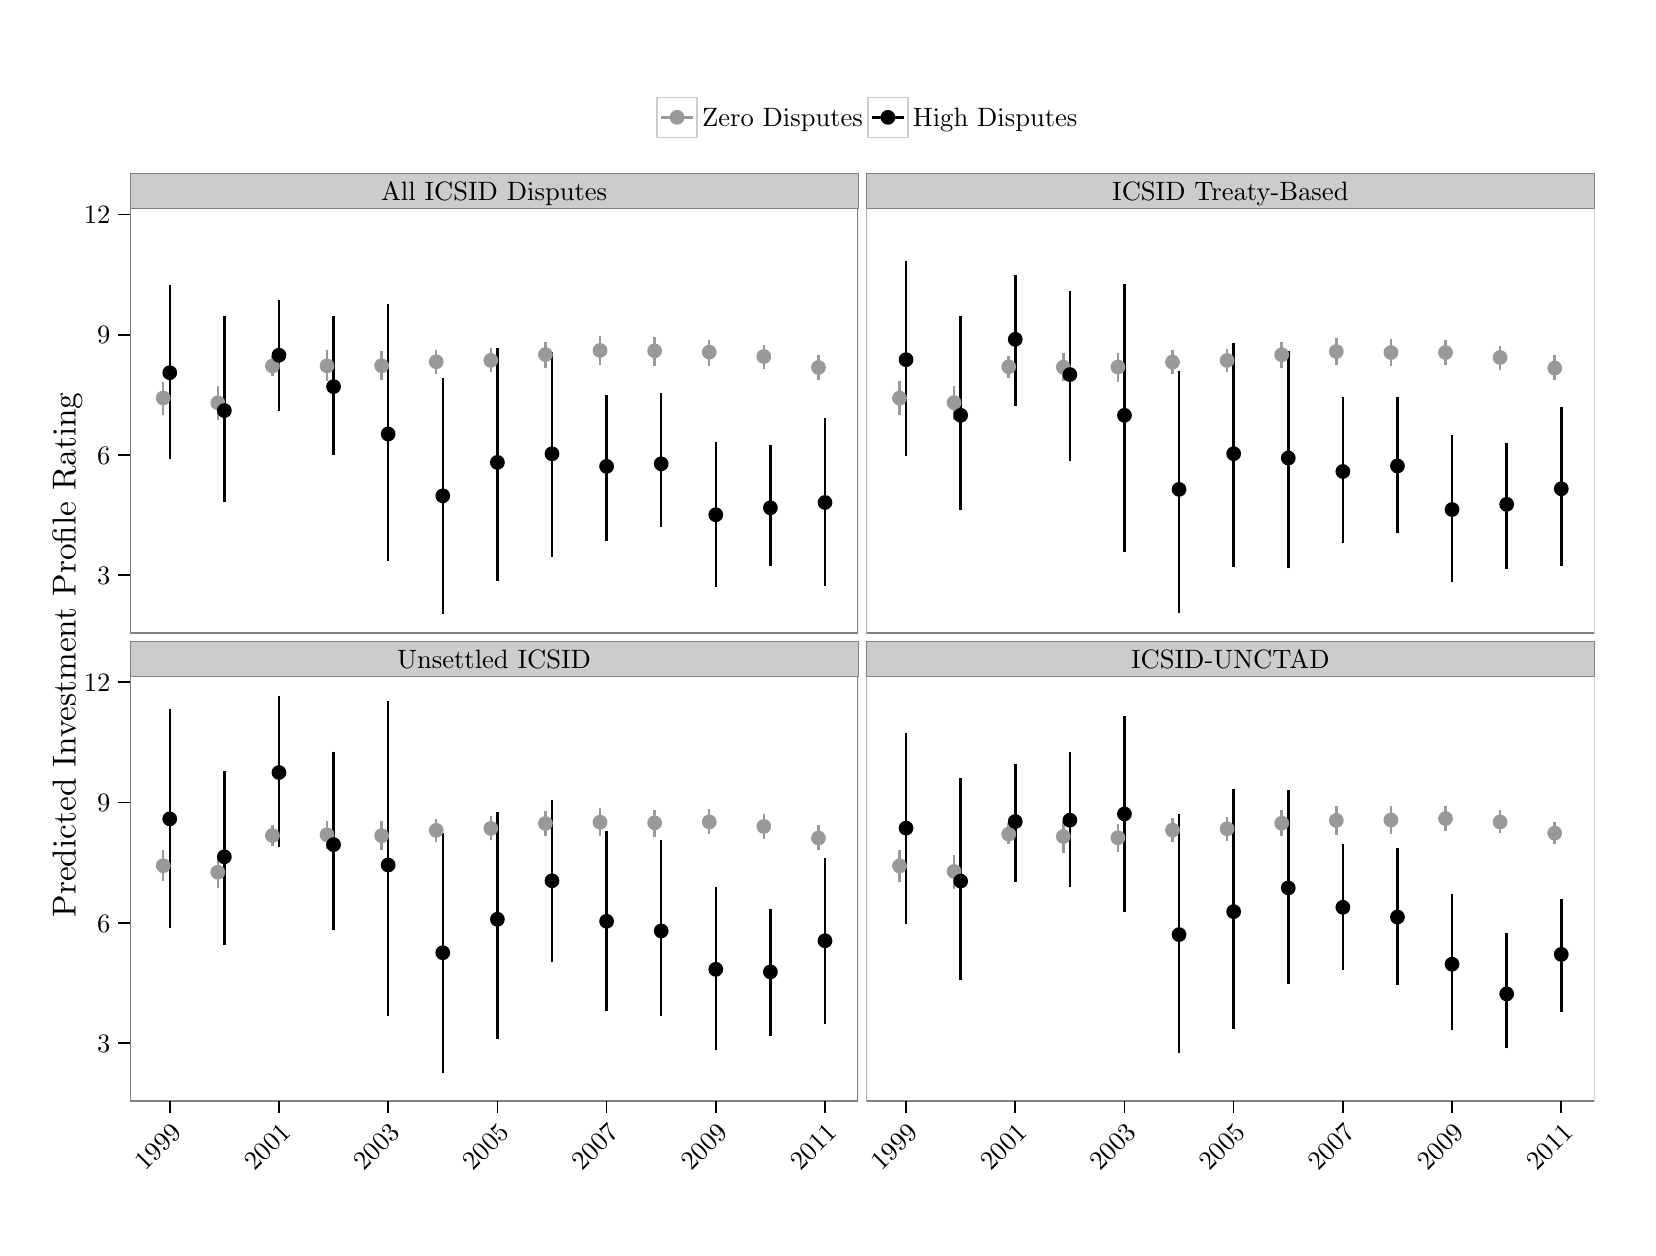
\begin{tikzpicture}[x=1pt,y=1pt]
\definecolor[named]{fillColor}{rgb}{1.00,1.00,1.00}
\path[use as bounding box,fill=fillColor,fill opacity=0.00] (0,0) rectangle (578.16,433.62);
\begin{scope}
\path[clip] (  0.00,  0.00) rectangle (578.16,433.62);
\definecolor[named]{drawColor}{rgb}{1.00,1.00,1.00}
\definecolor[named]{fillColor}{rgb}{1.00,1.00,1.00}

\path[draw=drawColor,line width= 0.6pt,line join=round,line cap=round,fill=fillColor] (  0.00,  0.00) rectangle (578.16,433.62);
\end{scope}
\begin{scope}
\path[clip] ( 37.02,214.77) rectangle (300.06,368.22);
\definecolor[named]{fillColor}{rgb}{1.00,1.00,1.00}

\path[fill=fillColor] ( 37.02,214.77) rectangle (300.06,368.22);
\definecolor[named]{drawColor}{rgb}{0.60,0.60,0.60}
\definecolor[named]{fillColor}{rgb}{0.60,0.60,0.60}

\path[draw=drawColor,line width= 0.9pt,line join=round,fill=fillColor] ( 48.98,293.67) -- ( 48.98,305.59);

\path[draw=drawColor,line width= 0.9pt,line join=round,fill=fillColor] ( 68.71,291.93) -- ( 68.71,304.29);

\path[draw=drawColor,line width= 0.9pt,line join=round,fill=fillColor] ( 88.44,307.70) -- ( 88.44,315.07);

\path[draw=drawColor,line width= 0.9pt,line join=round,fill=fillColor] (108.17,305.93) -- (108.17,317.28);

\path[draw=drawColor,line width= 0.9pt,line join=round,fill=fillColor] (127.90,306.46) -- (127.90,316.72);

\path[draw=drawColor,line width= 0.9pt,line join=round,fill=fillColor] (147.63,308.45) -- (147.63,317.07);

\path[draw=drawColor,line width= 0.9pt,line join=round,fill=fillColor] (167.36,309.24) -- (167.36,317.81);

\path[draw=drawColor,line width= 0.9pt,line join=round,fill=fillColor] (187.09,310.64) -- (187.09,320.16);

\path[draw=drawColor,line width= 0.9pt,line join=round,fill=fillColor] (206.82,311.61) -- (206.82,322.25);

\path[draw=drawColor,line width= 0.9pt,line join=round,fill=fillColor] (226.55,311.45) -- (226.55,321.98);

\path[draw=drawColor,line width= 0.9pt,line join=round,fill=fillColor] (246.28,311.52) -- (246.28,320.82);

\path[draw=drawColor,line width= 0.9pt,line join=round,fill=fillColor] (266.01,310.10) -- (266.01,319.07);

\path[draw=drawColor,line width= 0.9pt,line join=round,fill=fillColor] (285.74,306.38) -- (285.74,315.18);
\definecolor[named]{drawColor}{rgb}{0.00,0.00,0.00}
\definecolor[named]{fillColor}{rgb}{0.00,0.00,0.00}

\path[draw=drawColor,line width= 0.9pt,line join=round,fill=fillColor] ( 51.34,277.65) -- ( 51.34,340.81);

\path[draw=drawColor,line width= 0.9pt,line join=round,fill=fillColor] ( 71.07,262.34) -- ( 71.07,329.49);

\path[draw=drawColor,line width= 0.9pt,line join=round,fill=fillColor] ( 90.80,295.23) -- ( 90.80,335.12);

\path[draw=drawColor,line width= 0.9pt,line join=round,fill=fillColor] (110.53,279.19) -- (110.53,329.36);

\path[draw=drawColor,line width= 0.9pt,line join=round,fill=fillColor] (130.26,240.98) -- (130.26,333.61);

\path[draw=drawColor,line width= 0.9pt,line join=round,fill=fillColor] (150.00,221.74) -- (150.00,307.17);

\path[draw=drawColor,line width= 0.9pt,line join=round,fill=fillColor] (169.73,233.78) -- (169.73,317.86);

\path[draw=drawColor,line width= 0.9pt,line join=round,fill=fillColor] (189.46,242.46) -- (189.46,316.24);

\path[draw=drawColor,line width= 0.9pt,line join=round,fill=fillColor] (209.19,248.30) -- (209.19,300.81);

\path[draw=drawColor,line width= 0.9pt,line join=round,fill=fillColor] (228.92,253.28) -- (228.92,301.49);

\path[draw=drawColor,line width= 0.9pt,line join=round,fill=fillColor] (248.65,231.43) -- (248.65,284.04);

\path[draw=drawColor,line width= 0.9pt,line join=round,fill=fillColor] (268.38,239.20) -- (268.38,282.77);

\path[draw=drawColor,line width= 0.9pt,line join=round,fill=fillColor] (288.11,231.84) -- (288.11,292.68);
\definecolor[named]{fillColor}{rgb}{0.60,0.60,0.60}

\path[fill=fillColor] ( 48.98,299.78) circle (  2.67);
\definecolor[named]{fillColor}{rgb}{0.00,0.00,0.00}

\path[fill=fillColor] ( 51.34,308.94) circle (  2.67);
\definecolor[named]{fillColor}{rgb}{0.60,0.60,0.60}

\path[fill=fillColor] ( 68.71,298.06) circle (  2.67);
\definecolor[named]{fillColor}{rgb}{0.00,0.00,0.00}

\path[fill=fillColor] ( 71.07,295.25) circle (  2.67);
\definecolor[named]{fillColor}{rgb}{0.60,0.60,0.60}

\path[fill=fillColor] ( 88.44,311.37) circle (  2.67);
\definecolor[named]{fillColor}{rgb}{0.00,0.00,0.00}

\path[fill=fillColor] ( 90.80,315.26) circle (  2.67);
\definecolor[named]{fillColor}{rgb}{0.60,0.60,0.60}

\path[fill=fillColor] (108.17,311.43) circle (  2.67);
\definecolor[named]{fillColor}{rgb}{0.00,0.00,0.00}

\path[fill=fillColor] (110.53,303.90) circle (  2.67);
\definecolor[named]{fillColor}{rgb}{0.60,0.60,0.60}

\path[fill=fillColor] (127.90,311.46) circle (  2.67);
\definecolor[named]{fillColor}{rgb}{0.00,0.00,0.00}

\path[fill=fillColor] (130.26,286.79) circle (  2.67);
\definecolor[named]{fillColor}{rgb}{0.60,0.60,0.60}

\path[fill=fillColor] (147.63,312.90) circle (  2.67);
\definecolor[named]{fillColor}{rgb}{0.00,0.00,0.00}

\path[fill=fillColor] (150.00,264.46) circle (  2.67);
\definecolor[named]{fillColor}{rgb}{0.60,0.60,0.60}

\path[fill=fillColor] (167.36,313.40) circle (  2.67);
\definecolor[named]{fillColor}{rgb}{0.00,0.00,0.00}

\path[fill=fillColor] (169.73,276.53) circle (  2.67);
\definecolor[named]{fillColor}{rgb}{0.60,0.60,0.60}

\path[fill=fillColor] (187.09,315.49) circle (  2.67);
\definecolor[named]{fillColor}{rgb}{0.00,0.00,0.00}

\path[fill=fillColor] (189.46,279.64) circle (  2.67);
\definecolor[named]{fillColor}{rgb}{0.60,0.60,0.60}

\path[fill=fillColor] (206.82,316.99) circle (  2.67);
\definecolor[named]{fillColor}{rgb}{0.00,0.00,0.00}

\path[fill=fillColor] (209.19,275.10) circle (  2.67);
\definecolor[named]{fillColor}{rgb}{0.60,0.60,0.60}

\path[fill=fillColor] (226.55,316.84) circle (  2.67);
\definecolor[named]{fillColor}{rgb}{0.00,0.00,0.00}

\path[fill=fillColor] (228.92,276.03) circle (  2.67);
\definecolor[named]{fillColor}{rgb}{0.60,0.60,0.60}

\path[fill=fillColor] (246.28,316.38) circle (  2.67);
\definecolor[named]{fillColor}{rgb}{0.00,0.00,0.00}

\path[fill=fillColor] (248.65,257.61) circle (  2.67);
\definecolor[named]{fillColor}{rgb}{0.60,0.60,0.60}

\path[fill=fillColor] (266.01,314.79) circle (  2.67);
\definecolor[named]{fillColor}{rgb}{0.00,0.00,0.00}

\path[fill=fillColor] (268.38,260.12) circle (  2.67);
\definecolor[named]{fillColor}{rgb}{0.60,0.60,0.60}

\path[fill=fillColor] (285.74,310.83) circle (  2.67);
\definecolor[named]{fillColor}{rgb}{0.00,0.00,0.00}

\path[fill=fillColor] (288.11,262.05) circle (  2.67);
\definecolor[named]{drawColor}{rgb}{0.50,0.50,0.50}

\path[draw=drawColor,line width= 0.6pt,line join=round,line cap=round] ( 37.02,214.77) rectangle (300.06,368.22);
\end{scope}
\begin{scope}
\path[clip] (303.07,214.77) rectangle (566.12,368.22);
\definecolor[named]{fillColor}{rgb}{1.00,1.00,1.00}

\path[fill=fillColor] (303.07,214.77) rectangle (566.12,368.22);
\definecolor[named]{drawColor}{rgb}{0.60,0.60,0.60}
\definecolor[named]{fillColor}{rgb}{0.60,0.60,0.60}

\path[draw=drawColor,line width= 0.9pt,line join=round,fill=fillColor] (315.03,293.78) -- (315.03,305.84);

\path[draw=drawColor,line width= 0.9pt,line join=round,fill=fillColor] (334.76,291.95) -- (334.76,304.13);

\path[draw=drawColor,line width= 0.9pt,line join=round,fill=fillColor] (354.49,307.16) -- (354.49,314.84);

\path[draw=drawColor,line width= 0.9pt,line join=round,fill=fillColor] (374.22,305.98) -- (374.22,316.10);

\path[draw=drawColor,line width= 0.9pt,line join=round,fill=fillColor] (393.95,305.73) -- (393.95,316.18);

\path[draw=drawColor,line width= 0.9pt,line join=round,fill=fillColor] (413.68,308.47) -- (413.68,316.99);

\path[draw=drawColor,line width= 0.9pt,line join=round,fill=fillColor] (433.41,309.08) -- (433.41,317.58);

\path[draw=drawColor,line width= 0.9pt,line join=round,fill=fillColor] (453.14,310.77) -- (453.14,319.96);

\path[draw=drawColor,line width= 0.9pt,line join=round,fill=fillColor] (472.87,311.76) -- (472.87,321.65);

\path[draw=drawColor,line width= 0.9pt,line join=round,fill=fillColor] (492.60,311.49) -- (492.60,321.25);

\path[draw=drawColor,line width= 0.9pt,line join=round,fill=fillColor] (512.33,311.80) -- (512.33,320.87);

\path[draw=drawColor,line width= 0.9pt,line join=round,fill=fillColor] (532.06,310.00) -- (532.06,318.75);

\path[draw=drawColor,line width= 0.9pt,line join=round,fill=fillColor] (551.79,306.27) -- (551.79,315.18);
\definecolor[named]{drawColor}{rgb}{0.00,0.00,0.00}
\definecolor[named]{fillColor}{rgb}{0.00,0.00,0.00}

\path[draw=drawColor,line width= 0.9pt,line join=round,fill=fillColor] (317.40,278.99) -- (317.40,349.30);

\path[draw=drawColor,line width= 0.9pt,line join=round,fill=fillColor] (337.13,259.18) -- (337.13,329.45);

\path[draw=drawColor,line width= 0.9pt,line join=round,fill=fillColor] (356.86,296.83) -- (356.86,344.32);

\path[draw=drawColor,line width= 0.9pt,line join=round,fill=fillColor] (376.59,276.90) -- (376.59,338.49);

\path[draw=drawColor,line width= 0.9pt,line join=round,fill=fillColor] (396.32,243.99) -- (396.32,340.82);

\path[draw=drawColor,line width= 0.9pt,line join=round,fill=fillColor] (416.05,221.97) -- (416.05,309.69);

\path[draw=drawColor,line width= 0.9pt,line join=round,fill=fillColor] (435.78,238.83) -- (435.78,319.61);

\path[draw=drawColor,line width= 0.9pt,line join=round,fill=fillColor] (455.51,238.22) -- (455.51,316.91);

\path[draw=drawColor,line width= 0.9pt,line join=round,fill=fillColor] (475.24,247.41) -- (475.24,300.28);

\path[draw=drawColor,line width= 0.9pt,line join=round,fill=fillColor] (494.97,251.06) -- (494.97,300.07);

\path[draw=drawColor,line width= 0.9pt,line join=round,fill=fillColor] (514.70,233.31) -- (514.70,286.29);

\path[draw=drawColor,line width= 0.9pt,line join=round,fill=fillColor] (534.43,238.00) -- (534.43,283.55);

\path[draw=drawColor,line width= 0.9pt,line join=round,fill=fillColor] (554.16,238.96) -- (554.16,296.55);
\definecolor[named]{fillColor}{rgb}{0.60,0.60,0.60}

\path[fill=fillColor] (315.03,299.76) circle (  2.67);
\definecolor[named]{fillColor}{rgb}{0.00,0.00,0.00}

\path[fill=fillColor] (317.40,313.65) circle (  2.67);
\definecolor[named]{fillColor}{rgb}{0.60,0.60,0.60}

\path[fill=fillColor] (334.76,298.12) circle (  2.67);
\definecolor[named]{fillColor}{rgb}{0.00,0.00,0.00}

\path[fill=fillColor] (337.13,293.55) circle (  2.67);
\definecolor[named]{fillColor}{rgb}{0.60,0.60,0.60}

\path[fill=fillColor] (354.49,311.08) circle (  2.67);
\definecolor[named]{fillColor}{rgb}{0.00,0.00,0.00}

\path[fill=fillColor] (356.86,321.00) circle (  2.67);
\definecolor[named]{fillColor}{rgb}{0.60,0.60,0.60}

\path[fill=fillColor] (374.22,310.94) circle (  2.67);
\definecolor[named]{fillColor}{rgb}{0.00,0.00,0.00}

\path[fill=fillColor] (376.59,308.26) circle (  2.67);
\definecolor[named]{fillColor}{rgb}{0.60,0.60,0.60}

\path[fill=fillColor] (393.95,310.98) circle (  2.67);
\definecolor[named]{fillColor}{rgb}{0.00,0.00,0.00}

\path[fill=fillColor] (396.32,293.54) circle (  2.67);
\definecolor[named]{fillColor}{rgb}{0.60,0.60,0.60}

\path[fill=fillColor] (413.68,312.77) circle (  2.67);
\definecolor[named]{fillColor}{rgb}{0.00,0.00,0.00}

\path[fill=fillColor] (416.05,266.78) circle (  2.67);
\definecolor[named]{fillColor}{rgb}{0.60,0.60,0.60}

\path[fill=fillColor] (433.41,313.37) circle (  2.67);
\definecolor[named]{fillColor}{rgb}{0.00,0.00,0.00}

\path[fill=fillColor] (435.78,279.67) circle (  2.67);
\definecolor[named]{fillColor}{rgb}{0.60,0.60,0.60}

\path[fill=fillColor] (453.14,315.42) circle (  2.67);
\definecolor[named]{fillColor}{rgb}{0.00,0.00,0.00}

\path[fill=fillColor] (455.51,278.10) circle (  2.67);
\definecolor[named]{fillColor}{rgb}{0.60,0.60,0.60}

\path[fill=fillColor] (472.87,316.62) circle (  2.67);
\definecolor[named]{fillColor}{rgb}{0.00,0.00,0.00}

\path[fill=fillColor] (475.24,273.25) circle (  2.67);
\definecolor[named]{fillColor}{rgb}{0.60,0.60,0.60}

\path[fill=fillColor] (492.60,316.22) circle (  2.67);
\definecolor[named]{fillColor}{rgb}{0.00,0.00,0.00}

\path[fill=fillColor] (494.97,275.25) circle (  2.67);
\definecolor[named]{fillColor}{rgb}{0.60,0.60,0.60}

\path[fill=fillColor] (512.33,316.24) circle (  2.67);
\definecolor[named]{fillColor}{rgb}{0.00,0.00,0.00}

\path[fill=fillColor] (514.70,259.49) circle (  2.67);
\definecolor[named]{fillColor}{rgb}{0.60,0.60,0.60}

\path[fill=fillColor] (532.06,314.44) circle (  2.67);
\definecolor[named]{fillColor}{rgb}{0.00,0.00,0.00}

\path[fill=fillColor] (534.43,261.38) circle (  2.67);
\definecolor[named]{fillColor}{rgb}{0.60,0.60,0.60}

\path[fill=fillColor] (551.79,310.60) circle (  2.67);
\definecolor[named]{fillColor}{rgb}{0.00,0.00,0.00}

\path[fill=fillColor] (554.16,266.99) circle (  2.67);
\definecolor[named]{drawColor}{rgb}{0.50,0.50,0.50}

\path[draw=drawColor,line width= 0.6pt,line join=round,line cap=round] (303.07,214.77) rectangle (566.12,368.22);
\end{scope}
\begin{scope}
\path[clip] ( 37.02, 45.67) rectangle (300.06,199.12);
\definecolor[named]{fillColor}{rgb}{1.00,1.00,1.00}

\path[fill=fillColor] ( 37.02, 45.67) rectangle (300.06,199.12);
\definecolor[named]{drawColor}{rgb}{0.60,0.60,0.60}
\definecolor[named]{fillColor}{rgb}{0.60,0.60,0.60}

\path[draw=drawColor,line width= 0.9pt,line join=round,fill=fillColor] ( 48.98,125.38) -- ( 48.98,136.64);

\path[draw=drawColor,line width= 0.9pt,line join=round,fill=fillColor] ( 68.71,122.62) -- ( 68.71,134.68);

\path[draw=drawColor,line width= 0.9pt,line join=round,fill=fillColor] ( 88.44,137.99) -- ( 88.44,145.38);

\path[draw=drawColor,line width= 0.9pt,line join=round,fill=fillColor] (108.17,136.92) -- (108.17,146.80);

\path[draw=drawColor,line width= 0.9pt,line join=round,fill=fillColor] (127.90,136.43) -- (127.90,146.97);

\path[draw=drawColor,line width= 0.9pt,line join=round,fill=fillColor] (147.63,139.21) -- (147.63,147.84);

\path[draw=drawColor,line width= 0.9pt,line join=round,fill=fillColor] (167.36,139.98) -- (167.36,148.92);

\path[draw=drawColor,line width= 0.9pt,line join=round,fill=fillColor] (187.09,141.35) -- (187.09,150.56);

\path[draw=drawColor,line width= 0.9pt,line join=round,fill=fillColor] (206.82,141.52) -- (206.82,151.53);

\path[draw=drawColor,line width= 0.9pt,line join=round,fill=fillColor] (226.55,141.08) -- (226.55,151.10);

\path[draw=drawColor,line width= 0.9pt,line join=round,fill=fillColor] (246.28,142.10) -- (246.28,151.31);

\path[draw=drawColor,line width= 0.9pt,line join=round,fill=fillColor] (266.01,140.56) -- (266.01,149.61);

\path[draw=drawColor,line width= 0.9pt,line join=round,fill=fillColor] (285.74,136.44) -- (285.74,145.36);
\definecolor[named]{drawColor}{rgb}{0.00,0.00,0.00}
\definecolor[named]{fillColor}{rgb}{0.00,0.00,0.00}

\path[draw=drawColor,line width= 0.9pt,line join=round,fill=fillColor] ( 51.34,108.37) -- ( 51.34,187.25);

\path[draw=drawColor,line width= 0.9pt,line join=round,fill=fillColor] ( 71.07,102.13) -- ( 71.07,165.18);

\path[draw=drawColor,line width= 0.9pt,line join=round,fill=fillColor] ( 90.80,137.47) -- ( 90.80,192.15);

\path[draw=drawColor,line width= 0.9pt,line join=round,fill=fillColor] (110.53,107.39) -- (110.53,171.99);

\path[draw=drawColor,line width= 0.9pt,line join=round,fill=fillColor] (130.26, 76.50) -- (130.26,190.14);

\path[draw=drawColor,line width= 0.9pt,line join=round,fill=fillColor] (150.00, 55.81) -- (150.00,142.68);

\path[draw=drawColor,line width= 0.9pt,line join=round,fill=fillColor] (169.73, 68.20) -- (169.73,150.27);

\path[draw=drawColor,line width= 0.9pt,line join=round,fill=fillColor] (189.46, 95.95) -- (189.46,154.62);

\path[draw=drawColor,line width= 0.9pt,line join=round,fill=fillColor] (209.19, 78.21) -- (209.19,143.42);

\path[draw=drawColor,line width= 0.9pt,line join=round,fill=fillColor] (228.92, 76.53) -- (228.92,140.01);

\path[draw=drawColor,line width= 0.9pt,line join=round,fill=fillColor] (248.65, 64.08) -- (248.65,123.27);

\path[draw=drawColor,line width= 0.9pt,line join=round,fill=fillColor] (268.38, 69.38) -- (268.38,115.03);

\path[draw=drawColor,line width= 0.9pt,line join=round,fill=fillColor] (288.11, 73.63) -- (288.11,133.71);
\definecolor[named]{fillColor}{rgb}{0.60,0.60,0.60}

\path[fill=fillColor] ( 48.98,130.79) circle (  2.67);
\definecolor[named]{fillColor}{rgb}{0.00,0.00,0.00}

\path[fill=fillColor] ( 51.34,147.73) circle (  2.67);
\definecolor[named]{fillColor}{rgb}{0.60,0.60,0.60}

\path[fill=fillColor] ( 68.71,128.45) circle (  2.67);
\definecolor[named]{fillColor}{rgb}{0.00,0.00,0.00}

\path[fill=fillColor] ( 71.07,134.01) circle (  2.67);
\definecolor[named]{fillColor}{rgb}{0.60,0.60,0.60}

\path[fill=fillColor] ( 88.44,141.70) circle (  2.67);
\definecolor[named]{fillColor}{rgb}{0.00,0.00,0.00}

\path[fill=fillColor] ( 90.80,164.47) circle (  2.67);
\definecolor[named]{fillColor}{rgb}{0.60,0.60,0.60}

\path[fill=fillColor] (108.17,141.95) circle (  2.67);
\definecolor[named]{fillColor}{rgb}{0.00,0.00,0.00}

\path[fill=fillColor] (110.53,138.41) circle (  2.67);
\definecolor[named]{fillColor}{rgb}{0.60,0.60,0.60}

\path[fill=fillColor] (127.90,141.65) circle (  2.67);
\definecolor[named]{fillColor}{rgb}{0.00,0.00,0.00}

\path[fill=fillColor] (130.26,131.04) circle (  2.67);
\definecolor[named]{fillColor}{rgb}{0.60,0.60,0.60}

\path[fill=fillColor] (147.63,143.57) circle (  2.67);
\definecolor[named]{fillColor}{rgb}{0.00,0.00,0.00}

\path[fill=fillColor] (150.00, 99.35) circle (  2.67);
\definecolor[named]{fillColor}{rgb}{0.60,0.60,0.60}

\path[fill=fillColor] (167.36,144.27) circle (  2.67);
\definecolor[named]{fillColor}{rgb}{0.00,0.00,0.00}

\path[fill=fillColor] (169.73,111.43) circle (  2.67);
\definecolor[named]{fillColor}{rgb}{0.60,0.60,0.60}

\path[fill=fillColor] (187.09,146.06) circle (  2.67);
\definecolor[named]{fillColor}{rgb}{0.00,0.00,0.00}

\path[fill=fillColor] (189.46,125.36) circle (  2.67);
\definecolor[named]{fillColor}{rgb}{0.60,0.60,0.60}

\path[fill=fillColor] (206.82,146.52) circle (  2.67);
\definecolor[named]{fillColor}{rgb}{0.00,0.00,0.00}

\path[fill=fillColor] (209.19,110.72) circle (  2.67);
\definecolor[named]{fillColor}{rgb}{0.60,0.60,0.60}

\path[fill=fillColor] (226.55,146.28) circle (  2.67);
\definecolor[named]{fillColor}{rgb}{0.00,0.00,0.00}

\path[fill=fillColor] (228.92,107.22) circle (  2.67);
\definecolor[named]{fillColor}{rgb}{0.60,0.60,0.60}

\path[fill=fillColor] (246.28,146.63) circle (  2.67);
\definecolor[named]{fillColor}{rgb}{0.00,0.00,0.00}

\path[fill=fillColor] (248.65, 93.35) circle (  2.67);
\definecolor[named]{fillColor}{rgb}{0.60,0.60,0.60}

\path[fill=fillColor] (266.01,144.98) circle (  2.67);
\definecolor[named]{fillColor}{rgb}{0.00,0.00,0.00}

\path[fill=fillColor] (268.38, 92.43) circle (  2.67);
\definecolor[named]{fillColor}{rgb}{0.60,0.60,0.60}

\path[fill=fillColor] (285.74,140.79) circle (  2.67);
\definecolor[named]{fillColor}{rgb}{0.00,0.00,0.00}

\path[fill=fillColor] (288.11,103.67) circle (  2.67);
\definecolor[named]{drawColor}{rgb}{0.50,0.50,0.50}

\path[draw=drawColor,line width= 0.6pt,line join=round,line cap=round] ( 37.02, 45.67) rectangle (300.06,199.12);
\end{scope}
\begin{scope}
\path[clip] (303.07, 45.67) rectangle (566.12,199.12);
\definecolor[named]{fillColor}{rgb}{1.00,1.00,1.00}

\path[fill=fillColor] (303.07, 45.67) rectangle (566.12,199.12);
\definecolor[named]{drawColor}{rgb}{0.60,0.60,0.60}
\definecolor[named]{fillColor}{rgb}{0.60,0.60,0.60}

\path[draw=drawColor,line width= 0.9pt,line join=round,fill=fillColor] (315.03,124.77) -- (315.03,136.40);

\path[draw=drawColor,line width= 0.9pt,line join=round,fill=fillColor] (334.76,122.55) -- (334.76,134.49);

\path[draw=drawColor,line width= 0.9pt,line join=round,fill=fillColor] (354.49,138.58) -- (354.49,146.09);

\path[draw=drawColor,line width= 0.9pt,line join=round,fill=fillColor] (374.22,135.46) -- (374.22,146.59);

\path[draw=drawColor,line width= 0.9pt,line join=round,fill=fillColor] (393.95,135.88) -- (393.95,145.95);

\path[draw=drawColor,line width= 0.9pt,line join=round,fill=fillColor] (413.68,139.39) -- (413.68,147.97);

\path[draw=drawColor,line width= 0.9pt,line join=round,fill=fillColor] (433.41,139.78) -- (433.41,148.45);

\path[draw=drawColor,line width= 0.9pt,line join=round,fill=fillColor] (453.14,141.53) -- (453.14,150.88);

\path[draw=drawColor,line width= 0.9pt,line join=round,fill=fillColor] (472.87,141.91) -- (472.87,152.29);

\path[draw=drawColor,line width= 0.9pt,line join=round,fill=fillColor] (492.60,142.20) -- (492.60,152.36);

\path[draw=drawColor,line width= 0.9pt,line join=round,fill=fillColor] (512.33,143.35) -- (512.33,152.28);

\path[draw=drawColor,line width= 0.9pt,line join=round,fill=fillColor] (532.06,142.45) -- (532.06,150.85);

\path[draw=drawColor,line width= 0.9pt,line join=round,fill=fillColor] (551.79,138.48) -- (551.79,146.68);
\definecolor[named]{drawColor}{rgb}{0.00,0.00,0.00}
\definecolor[named]{fillColor}{rgb}{0.00,0.00,0.00}

\path[draw=drawColor,line width= 0.9pt,line join=round,fill=fillColor] (317.40,109.70) -- (317.40,178.73);

\path[draw=drawColor,line width= 0.9pt,line join=round,fill=fillColor] (337.13, 89.60) -- (337.13,162.56);

\path[draw=drawColor,line width= 0.9pt,line join=round,fill=fillColor] (356.86,124.91) -- (356.86,167.47);

\path[draw=drawColor,line width= 0.9pt,line join=round,fill=fillColor] (376.59,122.92) -- (376.59,171.79);

\path[draw=drawColor,line width= 0.9pt,line join=round,fill=fillColor] (396.32,113.96) -- (396.32,184.97);

\path[draw=drawColor,line width= 0.9pt,line join=round,fill=fillColor] (416.05, 62.98) -- (416.05,149.42);

\path[draw=drawColor,line width= 0.9pt,line join=round,fill=fillColor] (435.78, 71.72) -- (435.78,158.52);

\path[draw=drawColor,line width= 0.9pt,line join=round,fill=fillColor] (455.51, 88.23) -- (455.51,158.15);

\path[draw=drawColor,line width= 0.9pt,line join=round,fill=fillColor] (475.24, 93.25) -- (475.24,138.81);

\path[draw=drawColor,line width= 0.9pt,line join=round,fill=fillColor] (494.97, 87.78) -- (494.97,137.21);

\path[draw=drawColor,line width= 0.9pt,line join=round,fill=fillColor] (514.70, 71.48) -- (514.70,120.63);

\path[draw=drawColor,line width= 0.9pt,line join=round,fill=fillColor] (534.43, 64.78) -- (534.43,106.32);

\path[draw=drawColor,line width= 0.9pt,line join=round,fill=fillColor] (554.16, 77.99) -- (554.16,118.94);
\definecolor[named]{fillColor}{rgb}{0.60,0.60,0.60}

\path[fill=fillColor] (315.03,130.70) circle (  2.67);
\definecolor[named]{fillColor}{rgb}{0.00,0.00,0.00}

\path[fill=fillColor] (317.40,144.37) circle (  2.67);
\definecolor[named]{fillColor}{rgb}{0.60,0.60,0.60}

\path[fill=fillColor] (334.76,128.73) circle (  2.67);
\definecolor[named]{fillColor}{rgb}{0.00,0.00,0.00}

\path[fill=fillColor] (337.13,125.24) circle (  2.67);
\definecolor[named]{fillColor}{rgb}{0.60,0.60,0.60}

\path[fill=fillColor] (354.49,142.20) circle (  2.67);
\definecolor[named]{fillColor}{rgb}{0.00,0.00,0.00}

\path[fill=fillColor] (356.86,146.75) circle (  2.67);
\definecolor[named]{fillColor}{rgb}{0.60,0.60,0.60}

\path[fill=fillColor] (374.22,141.34) circle (  2.67);
\definecolor[named]{fillColor}{rgb}{0.00,0.00,0.00}

\path[fill=fillColor] (376.59,147.24) circle (  2.67);
\definecolor[named]{fillColor}{rgb}{0.60,0.60,0.60}

\path[fill=fillColor] (393.95,140.90) circle (  2.67);
\definecolor[named]{fillColor}{rgb}{0.00,0.00,0.00}

\path[fill=fillColor] (396.32,149.51) circle (  2.67);
\definecolor[named]{fillColor}{rgb}{0.60,0.60,0.60}

\path[fill=fillColor] (413.68,143.66) circle (  2.67);
\definecolor[named]{fillColor}{rgb}{0.00,0.00,0.00}

\path[fill=fillColor] (416.05,105.90) circle (  2.67);
\definecolor[named]{fillColor}{rgb}{0.60,0.60,0.60}

\path[fill=fillColor] (433.41,144.13) circle (  2.67);
\definecolor[named]{fillColor}{rgb}{0.00,0.00,0.00}

\path[fill=fillColor] (435.78,114.21) circle (  2.67);
\definecolor[named]{fillColor}{rgb}{0.60,0.60,0.60}

\path[fill=fillColor] (453.14,146.15) circle (  2.67);
\definecolor[named]{fillColor}{rgb}{0.00,0.00,0.00}

\path[fill=fillColor] (455.51,122.77) circle (  2.67);
\definecolor[named]{fillColor}{rgb}{0.60,0.60,0.60}

\path[fill=fillColor] (472.87,147.15) circle (  2.67);
\definecolor[named]{fillColor}{rgb}{0.00,0.00,0.00}

\path[fill=fillColor] (475.24,115.76) circle (  2.67);
\definecolor[named]{fillColor}{rgb}{0.60,0.60,0.60}

\path[fill=fillColor] (492.60,147.30) circle (  2.67);
\definecolor[named]{fillColor}{rgb}{0.00,0.00,0.00}

\path[fill=fillColor] (494.97,112.25) circle (  2.67);
\definecolor[named]{fillColor}{rgb}{0.60,0.60,0.60}

\path[fill=fillColor] (512.33,147.83) circle (  2.67);
\definecolor[named]{fillColor}{rgb}{0.00,0.00,0.00}

\path[fill=fillColor] (514.70, 95.21) circle (  2.67);
\definecolor[named]{fillColor}{rgb}{0.60,0.60,0.60}

\path[fill=fillColor] (532.06,146.59) circle (  2.67);
\definecolor[named]{fillColor}{rgb}{0.00,0.00,0.00}

\path[fill=fillColor] (534.43, 84.49) circle (  2.67);
\definecolor[named]{fillColor}{rgb}{0.60,0.60,0.60}

\path[fill=fillColor] (551.79,142.58) circle (  2.67);
\definecolor[named]{fillColor}{rgb}{0.00,0.00,0.00}

\path[fill=fillColor] (554.16, 98.75) circle (  2.67);
\definecolor[named]{drawColor}{rgb}{0.50,0.50,0.50}

\path[draw=drawColor,line width= 0.6pt,line join=round,line cap=round] (303.07, 45.67) rectangle (566.12,199.12);
\end{scope}
\begin{scope}
\path[clip] (  0.00,  0.00) rectangle (578.16,433.62);
\definecolor[named]{drawColor}{rgb}{0.50,0.50,0.50}
\definecolor[named]{fillColor}{rgb}{0.80,0.80,0.80}

\path[draw=drawColor,line width= 0.2pt,line join=round,line cap=round,fill=fillColor] ( 37.02,368.22) rectangle (300.06,380.85);
\definecolor[named]{drawColor}{rgb}{0.00,0.00,0.00}

\node[text=drawColor,anchor=base,inner sep=0pt, outer sep=0pt, scale=  0.96] at (168.54,371.23) {All ICSID Disputes};
\end{scope}
\begin{scope}
\path[clip] (  0.00,  0.00) rectangle (578.16,433.62);
\definecolor[named]{drawColor}{rgb}{0.50,0.50,0.50}
\definecolor[named]{fillColor}{rgb}{0.80,0.80,0.80}

\path[draw=drawColor,line width= 0.2pt,line join=round,line cap=round,fill=fillColor] (303.07,368.22) rectangle (566.12,380.85);
\definecolor[named]{drawColor}{rgb}{0.00,0.00,0.00}

\node[text=drawColor,anchor=base,inner sep=0pt, outer sep=0pt, scale=  0.96] at (434.59,371.23) {ICSID Treaty-Based};
\end{scope}
\begin{scope}
\path[clip] (  0.00,  0.00) rectangle (578.16,433.62);
\definecolor[named]{drawColor}{rgb}{0.50,0.50,0.50}
\definecolor[named]{fillColor}{rgb}{0.80,0.80,0.80}

\path[draw=drawColor,line width= 0.2pt,line join=round,line cap=round,fill=fillColor] ( 37.02,199.12) rectangle (300.06,211.75);
\definecolor[named]{drawColor}{rgb}{0.00,0.00,0.00}

\node[text=drawColor,anchor=base,inner sep=0pt, outer sep=0pt, scale=  0.96] at (168.54,202.13) {Unsettled ICSID};
\end{scope}
\begin{scope}
\path[clip] (  0.00,  0.00) rectangle (578.16,433.62);
\definecolor[named]{drawColor}{rgb}{0.50,0.50,0.50}
\definecolor[named]{fillColor}{rgb}{0.80,0.80,0.80}

\path[draw=drawColor,line width= 0.2pt,line join=round,line cap=round,fill=fillColor] (303.07,199.12) rectangle (566.12,211.75);
\definecolor[named]{drawColor}{rgb}{0.00,0.00,0.00}

\node[text=drawColor,anchor=base,inner sep=0pt, outer sep=0pt, scale=  0.96] at (434.59,202.13) {ICSID-UNCTAD};
\end{scope}
\begin{scope}
\path[clip] (  0.00,  0.00) rectangle (578.16,433.62);
\definecolor[named]{drawColor}{rgb}{0.00,0.00,0.00}

\node[text=drawColor,anchor=base east,inner sep=0pt, outer sep=0pt, scale=  0.96] at ( 29.91,232.42) {3};

\node[text=drawColor,anchor=base east,inner sep=0pt, outer sep=0pt, scale=  0.96] at ( 29.91,275.90) {6};

\node[text=drawColor,anchor=base east,inner sep=0pt, outer sep=0pt, scale=  0.96] at ( 29.91,319.38) {9};

\node[text=drawColor,anchor=base east,inner sep=0pt, outer sep=0pt, scale=  0.96] at ( 29.91,362.86) {12};
\end{scope}
\begin{scope}
\path[clip] (  0.00,  0.00) rectangle (578.16,433.62);
\definecolor[named]{drawColor}{rgb}{0.00,0.00,0.00}

\path[draw=drawColor,line width= 0.6pt,line join=round] ( 32.75,235.73) --
	( 37.02,235.73);

\path[draw=drawColor,line width= 0.6pt,line join=round] ( 32.75,279.21) --
	( 37.02,279.21);

\path[draw=drawColor,line width= 0.6pt,line join=round] ( 32.75,322.68) --
	( 37.02,322.68);

\path[draw=drawColor,line width= 0.6pt,line join=round] ( 32.75,366.16) --
	( 37.02,366.16);
\end{scope}
\begin{scope}
\path[clip] (  0.00,  0.00) rectangle (578.16,433.62);
\definecolor[named]{drawColor}{rgb}{0.00,0.00,0.00}

\node[text=drawColor,anchor=base east,inner sep=0pt, outer sep=0pt, scale=  0.96] at ( 29.91, 63.33) {3};

\node[text=drawColor,anchor=base east,inner sep=0pt, outer sep=0pt, scale=  0.96] at ( 29.91,106.81) {6};

\node[text=drawColor,anchor=base east,inner sep=0pt, outer sep=0pt, scale=  0.96] at ( 29.91,150.28) {9};

\node[text=drawColor,anchor=base east,inner sep=0pt, outer sep=0pt, scale=  0.96] at ( 29.91,193.76) {12};
\end{scope}
\begin{scope}
\path[clip] (  0.00,  0.00) rectangle (578.16,433.62);
\definecolor[named]{drawColor}{rgb}{0.00,0.00,0.00}

\path[draw=drawColor,line width= 0.6pt,line join=round] ( 32.75, 66.63) --
	( 37.02, 66.63);

\path[draw=drawColor,line width= 0.6pt,line join=round] ( 32.75,110.11) --
	( 37.02,110.11);

\path[draw=drawColor,line width= 0.6pt,line join=round] ( 32.75,153.59) --
	( 37.02,153.59);

\path[draw=drawColor,line width= 0.6pt,line join=round] ( 32.75,197.07) --
	( 37.02,197.07);
\end{scope}
\begin{scope}
\path[clip] (  0.00,  0.00) rectangle (578.16,433.62);
\definecolor[named]{drawColor}{rgb}{0.00,0.00,0.00}

\path[draw=drawColor,line width= 0.6pt,line join=round] ( 51.34, 41.40) --
	( 51.34, 45.67);

\path[draw=drawColor,line width= 0.6pt,line join=round] ( 90.80, 41.40) --
	( 90.80, 45.67);

\path[draw=drawColor,line width= 0.6pt,line join=round] (130.26, 41.40) --
	(130.26, 45.67);

\path[draw=drawColor,line width= 0.6pt,line join=round] (169.73, 41.40) --
	(169.73, 45.67);

\path[draw=drawColor,line width= 0.6pt,line join=round] (209.19, 41.40) --
	(209.19, 45.67);

\path[draw=drawColor,line width= 0.6pt,line join=round] (248.65, 41.40) --
	(248.65, 45.67);

\path[draw=drawColor,line width= 0.6pt,line join=round] (288.11, 41.40) --
	(288.11, 45.67);
\end{scope}
\begin{scope}
\path[clip] (  0.00,  0.00) rectangle (578.16,433.62);
\definecolor[named]{drawColor}{rgb}{0.00,0.00,0.00}

\node[text=drawColor,rotate= 45.00,anchor=base east,inner sep=0pt, outer sep=0pt, scale=  0.96] at ( 56.02, 33.88) {1999};

\node[text=drawColor,rotate= 45.00,anchor=base east,inner sep=0pt, outer sep=0pt, scale=  0.96] at ( 95.48, 33.88) {2001};

\node[text=drawColor,rotate= 45.00,anchor=base east,inner sep=0pt, outer sep=0pt, scale=  0.96] at (134.94, 33.88) {2003};

\node[text=drawColor,rotate= 45.00,anchor=base east,inner sep=0pt, outer sep=0pt, scale=  0.96] at (174.40, 33.88) {2005};

\node[text=drawColor,rotate= 45.00,anchor=base east,inner sep=0pt, outer sep=0pt, scale=  0.96] at (213.86, 33.88) {2007};

\node[text=drawColor,rotate= 45.00,anchor=base east,inner sep=0pt, outer sep=0pt, scale=  0.96] at (253.32, 33.88) {2009};

\node[text=drawColor,rotate= 45.00,anchor=base east,inner sep=0pt, outer sep=0pt, scale=  0.96] at (292.78, 33.88) {2011};
\end{scope}
\begin{scope}
\path[clip] (  0.00,  0.00) rectangle (578.16,433.62);
\definecolor[named]{drawColor}{rgb}{0.00,0.00,0.00}

\path[draw=drawColor,line width= 0.6pt,line join=round] (317.40, 41.40) --
	(317.40, 45.67);

\path[draw=drawColor,line width= 0.6pt,line join=round] (356.86, 41.40) --
	(356.86, 45.67);

\path[draw=drawColor,line width= 0.6pt,line join=round] (396.32, 41.40) --
	(396.32, 45.67);

\path[draw=drawColor,line width= 0.6pt,line join=round] (435.78, 41.40) --
	(435.78, 45.67);

\path[draw=drawColor,line width= 0.6pt,line join=round] (475.24, 41.40) --
	(475.24, 45.67);

\path[draw=drawColor,line width= 0.6pt,line join=round] (514.70, 41.40) --
	(514.70, 45.67);

\path[draw=drawColor,line width= 0.6pt,line join=round] (554.16, 41.40) --
	(554.16, 45.67);
\end{scope}
\begin{scope}
\path[clip] (  0.00,  0.00) rectangle (578.16,433.62);
\definecolor[named]{drawColor}{rgb}{0.00,0.00,0.00}

\node[text=drawColor,rotate= 45.00,anchor=base east,inner sep=0pt, outer sep=0pt, scale=  0.96] at (322.07, 33.88) {1999};

\node[text=drawColor,rotate= 45.00,anchor=base east,inner sep=0pt, outer sep=0pt, scale=  0.96] at (361.53, 33.88) {2001};

\node[text=drawColor,rotate= 45.00,anchor=base east,inner sep=0pt, outer sep=0pt, scale=  0.96] at (400.99, 33.88) {2003};

\node[text=drawColor,rotate= 45.00,anchor=base east,inner sep=0pt, outer sep=0pt, scale=  0.96] at (440.45, 33.88) {2005};

\node[text=drawColor,rotate= 45.00,anchor=base east,inner sep=0pt, outer sep=0pt, scale=  0.96] at (479.91, 33.88) {2007};

\node[text=drawColor,rotate= 45.00,anchor=base east,inner sep=0pt, outer sep=0pt, scale=  0.96] at (519.37, 33.88) {2009};

\node[text=drawColor,rotate= 45.00,anchor=base east,inner sep=0pt, outer sep=0pt, scale=  0.96] at (558.83, 33.88) {2011};
\end{scope}
\begin{scope}
\path[clip] (  0.00,  0.00) rectangle (578.16,433.62);
\definecolor[named]{drawColor}{rgb}{0.00,0.00,0.00}

\node[text=drawColor,rotate= 90.00,anchor=base,inner sep=0pt, outer sep=0pt, scale=  1.20] at ( 17.30,206.94) {Predicted Investment Profile Rating};
\end{scope}
\begin{scope}
\path[clip] (  0.00,  0.00) rectangle (578.16,433.62);
\definecolor[named]{fillColor}{rgb}{1.00,1.00,1.00}

\path[fill=fillColor] (219.56,389.72) rectangle (383.58,412.71);
\end{scope}
\begin{scope}
\path[clip] (  0.00,  0.00) rectangle (578.16,433.62);
\definecolor[named]{drawColor}{rgb}{0.80,0.80,0.80}
\definecolor[named]{fillColor}{rgb}{1.00,1.00,1.00}

\path[draw=drawColor,line width= 0.6pt,line join=round,line cap=round,fill=fillColor] (227.44,393.99) rectangle (241.89,408.44);
\end{scope}
\begin{scope}
\path[clip] (  0.00,  0.00) rectangle (578.16,433.62);
\definecolor[named]{drawColor}{rgb}{0.60,0.60,0.60}

\path[draw=drawColor,line width= 0.9pt,line join=round] (228.88,401.21) -- (240.45,401.21);
\end{scope}
\begin{scope}
\path[clip] (  0.00,  0.00) rectangle (578.16,433.62);
\definecolor[named]{fillColor}{rgb}{0.60,0.60,0.60}

\path[fill=fillColor] (234.66,401.21) circle (  2.67);
\end{scope}
\begin{scope}
\path[clip] (  0.00,  0.00) rectangle (578.16,433.62);
\definecolor[named]{drawColor}{rgb}{0.80,0.80,0.80}
\definecolor[named]{fillColor}{rgb}{1.00,1.00,1.00}

\path[draw=drawColor,line width= 0.6pt,line join=round,line cap=round,fill=fillColor] (303.62,393.99) rectangle (318.08,408.44);
\end{scope}
\begin{scope}
\path[clip] (  0.00,  0.00) rectangle (578.16,433.62);
\definecolor[named]{drawColor}{rgb}{0.00,0.00,0.00}

\path[draw=drawColor,line width= 0.9pt,line join=round] (305.07,401.21) -- (316.63,401.21);
\end{scope}
\begin{scope}
\path[clip] (  0.00,  0.00) rectangle (578.16,433.62);
\definecolor[named]{fillColor}{rgb}{0.00,0.00,0.00}

\path[fill=fillColor] (310.85,401.21) circle (  2.67);
\end{scope}
\begin{scope}
\path[clip] (  0.00,  0.00) rectangle (578.16,433.62);
\definecolor[named]{drawColor}{rgb}{0.00,0.00,0.00}

\node[text=drawColor,anchor=base west,inner sep=0pt, outer sep=0pt, scale=  0.96] at (243.70,397.91) {Zero Disputes};
\end{scope}
\begin{scope}
\path[clip] (  0.00,  0.00) rectangle (578.16,433.62);
\definecolor[named]{drawColor}{rgb}{0.00,0.00,0.00}

\node[text=drawColor,anchor=base west,inner sep=0pt, outer sep=0pt, scale=  0.96] at (319.89,397.91) {High Disputes};
\end{scope}
\end{tikzpicture}
}	
\end{figure}

\end{frame}
%%%%%%%%%%%%%%%%%%%%%%%%%%%%%%%%%%%%%%%%%

%%%%%%%%%%%%%%%%%%%%%%%%%%%%%%%%%%%%%%%%%
\begin{frame}
\frametitle{Newspaper Mentions of ICSID}

\begin{figure}[ht]
	\centering
	\resizebox{1\textwidth}{!}{\input{histICSID}}
\end{figure}

\end{frame}
%%%%%%%%%%%%%%%%%%%%%%%%%%%%%%%%%%%%%%%%%

%%%%%%%%%%%%%%%%%%%%%%%%%%%%%%%%%%%%%%%%%
\begin{frame}
\frametitle{Listing of web-based services monitoring ICSID processes}

\begin{table}[ht]
\centering
\begin{tabular}{lc}
	\hline\hline
	Source & Year Established \\
	\hline
	Investment Treaty News & 2002 \\
	Transnational Dispute Management & 2003 \\
	Investment Treaty Arbitration & 2004 \\
	Global Arbitration Review & 2006 \\
	Investment Arbitration Reporter & 2008 \\
	International Arbitration Database & 2008 \\
	Kluwer Arbitration Blog & 2009 \\
	Investor-State LawGuide & 2011 \\
	International Investment Arbitration & 2011 \\
	\hline\hline
\end{tabular}
\end{table}

\end{frame}
%%%%%%%%%%%%%%%%%%%%%%%%%%%%%%%%%%%%%%%%%

\section{Conclusion}

%%%%%%%%%%%%%%%%%%%%%%%%%%%%%%%%%%%%%%%%%
\begin{frame}
\frametitle{}

\begin{center}
Thanks for your time!
\end{center}

\end{frame}
%%%%%%%%%%%%%%%%%%%%%%%%%%%%%%%%%%%%%%%%%

\end{document}